\documentclass[a4paper,twoside]{book}
\usepackage{geometry}
\usepackage[notheorems]{beamerarticle}

\makeindex

\mode<presentation>{
  % \useinnertheme{rectangles}
  %\useoutertheme{infolines}
  % \usecolortheme{crane}
  % \usecolortheme{rose}
}

\documentclass{article}

\usepackage[utf8]{inputenc}
\usepackage[english]{babel}

\usepackage{graphicx}
\usepackage{float}
\usepackage{amsmath}

\usepackage{hyperref}
\hypersetup{
    colorlinks=true,
    linkcolor=blue,
    filecolor=magenta,
    urlcolor=violet
}

\title{IN-STK5000 Project 2 Report}

\author{...}

\date{Fall 2020}

%\includeonly{causality}
\title{Machine learning in science and society}
\subtitle{From automated science to beneficial artificial intelligence}
\author[C. Dimitrakakis]{Christos Dimitrakakis}
\begin{document}

\maketitle
\tableofcontents

\chapter{Introduction}
\label{ch:introduction}
\include{ml-intro}

\chapter{Simple decision problems}
\label{ch:decision-problems}
\only<article>{This chapter deals with simple decision problems, whereby a decision maker (DM) makes a simple choice among many. In some of this problems the DM has to make a decision after first observing some side-information. Then the DM uses a \emph{decision rule} to assign a probability to each possible decision for each possible side-information. However, designing the decision rule is not trivial, as it relies on previously collected data. A higher-level decision includes choosing the decision rule itself. The problems of classification and regression fall within this framework. While most steps in the process can be automated and formalised, a lot of decisions are actual design choices made by humans. This creates scope for errors and misinterpretation of results.

In this chapter, we shall formalise all these simple decision problems from the point of view of statistical decision theory. The first question is, given a real world application, what type of decision problem does it map to? Then, what kind of machine learning algorithms can we use to solve it? What are the underlying assumptions and how valid are our conclusions? 
}

\include{knn}  % knn, reproducability and bootstrapping
\section{Reproducibility}
\only<presentation>{
  \begin{frame}
    \tableofcontents[ 
    currentsection, 
    hideothersubsections, 
    sectionstyle=show/shaded
    ] 
  \end{frame}
}
\begin{frame}
  \only<article>{ One of the main problems in science is
    reproducibility: when we are trying to draw conclusions from one
    specific data set, it is easy to make a mistake. For that reason,
    the scientific process requires us to use our conclusions to make
    testable predictions, and then test those predictions with new
    experiments. These new experiments should bear out the results of
    the previous experiments.  In more detail, reproducibility can be
    thought of as two different aspects of answering the question ``can this research be replicated?''}


  \begin{block}{Computational reproducibility: Can the study be repeated?}
    Can we, from the available information and data, exactly reproduce the reported methods and results?

    \only<article>{This is something that is useful to be able to even to the original authors of a study. The standard method for achieving this is using version control tools so that the exact version of algorithms, text and data used to write up the study is appropriately labelled. Ideally, any other researcher should be able to run a single script to reproduce all of the study and its computations. The following tools are going to be used in this course:}

    \begin{itemize}
    \item \texttt{jupyter} notebooks \only<article>{for interactive note taking.}
    \item \texttt{svn}, \texttt{git} or \texttt{mercurial} version control systems \only<article>{for tracking versions, changes and collaborating with others.}
    \end{itemize}
  \end{block}

  \begin{block}{Scientific reproducibility: Is the conclusion correct?}
    Can we, from the available information and a \alert{new} set of data, reproduce the conclusions of the original study?

     \only<article>{Here followup research may involve using exactly the same methods. In AI research would mean for example testing whether an algorithm is really performing as well as it is claimed, by testing it in new problems. This can involve a re-implementation. In more general scientific research, it might be the case that the methodology proposed by an original study is flawed, and so a better method should be used to draw better conclusions. Or it might simply be that more data is needed.}
  \end{block}

  When publishing results about a \alert{new method}, computational reproducibility is essential for scientific reproducibility.
\end{frame}


\begin{frame}

  \includegraphics[width=\textwidth]{../figures/2016-election}
  \only<article>{A simple example is the 2016 presidential election in the United States, where polling forecasts were not able to predict the outcome. In general, while we can make models about people's opinions regarding candidates in order to predict voting totals, the test of these models comes in the actual election. Unfortunately the only way we have of tuning our models is on previous elections, which are not that frequent, and on the results of previous polls. In addition, predicting the winner of an election is slightly different from predicting how many people are prepared to vote for them across the country. This, together with other factors such as shifting opinions, motivation and how close the sampling distribution is to the voting distribution have a significant effect on accuracy.}
  
\end{frame}
\begin{frame}
  \only<article>{The same thing can be done in when dealing purely
    with data, by making sure we use some of the data as input to the
    algorithm, and other data to measure the quality of the algorithm
    itself. In the following, we assume we have some algorithm
    $\alg : \Datasets \to \Pol$, where $\Datasets$ is the universe of
    possible input data and $\Pol$ the possible outputs, e.g. all
    possible classification policies. We also assume the existence of
    some quality measure $U$. How should we measure the quality of our
    algorithmic choices? 
    
    Take classification as an example. For a given training set, simply memorising all the labels of each example gives us perfect performance on the training set. Intuitively, this is not a good measure of performance, as we'd probably get poor results on a freshly sampled set. We can think of the training data as input to an algorithm, and the resulting classifier as the algorithm output. The evaluation function also requires some data in order to measure the performance of the policy. This can be expressed into the following principle.
  }
  \begin{alertblock}{The principle of independent evaluation}    
    Data used for estimation cannot be used for evaluation.
  \end{alertblock}
  \only<article>{This applies both to computer-implemented and human-implemented algorithms.}
\end{frame}


\begin{frame}
  \begin{figure}[H]
    \begin{center}
      \begin{tikzpicture}[line width=2pt]
        \onslide<1->{
          \node[select,label=above:Data Collection] at (0,2) (experiment) {$\chi$};
        }
        \onslide<2->{
          \node[RV,label=above:Training] at (4,2) (training) {$\Training$};
          \draw[blue,->] (experiment) -- (training);
        }
        \onslide<3->{
          \node[select,label=below:{Algorithm, hyperparameters}] at (0,0) (alg) {$\alg$};
        }
        \onslide<4->{
          \node[RV,label=below:Classifier] at (4,0) (pol) {$\pol$};
          \draw[red,->,dashed] (experiment) -- (pol);
          \draw[red,->] (alg) -- (pol);
          \draw[red,->] (training) -- (pol);
        }
        \onslide<5->{
          \node[RV,label=above:Holdout] at (8,2) (holdout) {$\Holdout$};
        }
        \onslide<6->{
          \draw[blue,->] (experiment) to [bend left=45] (holdout);
        }
        \onslide<7->{
          \node[utility,label=below:Measurement] at (8,0) (util) {$\util$};
          \draw[red,->] (pol) -- (util);
          \draw[red,->] (holdout) -- (util);
        }
      \end{tikzpicture}
    \end{center}
    \caption{The decision process in classification.}
  \end{figure}
  \only<article>{One can think of the decision process in classification as follows. First, we decide to collect some data according to some experimental protocol $\chi$. We also decide to use some algorithm (with associated hyperparameters) $\alg$ together with data $\Training$ we will obtain from our data collection in order to obtain a classification policy $\pol$.\index{policy!classification} Typically, we need to measure the quality of a policy according to how well it classifies on unknown data. This is because our policy has been generated using $\Training$, and so any measurement of its quality using the same data $\Training$, is going to be biased.

    \paragraph{Classification accuracy.} For classification problems, there is a natural metric $U$ to measure: The classification accuracy of the classifier. If the classification decisions are stochastic, then the classifier assigns probability $\pol(a \mid x)$ to each possible label $a$, and our utility is simply the identity function $U(a, y) \defn \ind{a = y}$. 
  }
  \uncover<8->{
    \begin{block}{Classification accuracy}
      \only<article>{
        For any fixed classifier $\pol$, the classification accuracy under the data distribution $\chi$ is:}
      \only<8>{
      \[
      \E_\chi[\util(\pol)] = \sum_{x,y} \underset{\textrm{Data probability}}{\underbrace{\Pr_\chi(x, y)}} \overset{\textrm{Decision probability}}{\overbrace{\pol(a = y \mid x)}}
      \]
      }
      \only<article>{The classification accuracy of policy $\pol$ under $\chi$ is the expected number of times the policy decides $\pol$ chooses the correct class. However, when approximating $\chi$ with a sample $\Holdout$, we instead obtain the empirical estimate:}\index{policy!classification accuracy}
      \only<9>{
      \[
      \E_{\Holdout} \util(\pol) = \sum_{(x,y) \in \Holdout} \pol(a = y \mid x) / |\Holdout|.
      \]
      }
    \end{block}
  }
  \only<article>{Of course, there is no reason to limit ourselves to the identity function. The utility could very well be such that some errors are penalised more than other errors. Consider for example an intrusion detection scenario: it is probably more important to correctly classify intrusions. This can be taken into account by weighing correct decisions about intrusions more relative to correct decisions about normal data.  }
\end{frame}

\subsection{The human as an algorithm}
\begin{frame}
  \frametitle{The human as an algorithm.}
  \only<article>{The same way with which an algorithm creates a model from some prior assumptions and data, so can a human select an algorithm and associated hyperparamters by executing an algorithm herself. This involves trying different algorithms and hyperparametrs on the same training data $\Training$ and then measuring their performance in the holdout set $\Holdout$.}
  \begin{figure}[H]
  \centering
  \begin{tikzpicture}[line width=2pt]
    \node[select,label=above:Data Collection] at (0,2) (experiment) {$\chi$};
    \node[RV,label=above:Training] at (4,2) (training) {$\Training$};
    \node[RV,label=above:Holdout] at (8,2) (holdout) {$\Holdout$};
     \draw[blue,->] (experiment) -- (training);
    \draw[blue,->] (experiment) to [bend left=45] (holdout);
    \node<2->[select,label=below:{Algorithm, hyperparameters}] at (0,0) (alg) {$\alg_1$};     
    \node<3->[RV,label=below:Classifier] at (4,0) (pol) {$\pol_1$};
    \draw<3->[red,->] (alg) -- (pol);
    \draw<3->[red,->] (training) -- (pol);
    \node<4->[utility,label=below:Measurement] at (8,0) (util) {$\util_1$};
    \draw<4->[red,->] (pol) -- (util);
    \draw<4->[red,->] (holdout) -- (util);
    \node<5->[select,label=below:{Algorithm, hyperparameters}] at (0,-2) (alg2) {$\alg_2$};
    \node<6->[RV,label=below:Classifier] at (4,-2) (pol2) {$\pol_2$};
    \node<7->[utility,label=below:Measurement] at (8,-2) (util2) {$\util_2$};
    \draw<6->[red,->] (alg2) -- (pol2);
    \draw<6->[red,->] (training) to [bend left] (pol2);
    \draw<7->[red,->] (pol2) -- (util2);
    \draw<7->[red,->] (holdout) to [bend right] (util2);
  \end{tikzpicture}
    \caption{Selecting algorithms and hyperparameters through holdouts}
    \label{fig:human-as-algorithm}
  \end{figure}

\end{frame}

\begin{frame}
  \frametitle{Holdout sets}
  \only<article>{To summarise, holdout sets are used in order to be able to evaluate the performance of specific algorithms, or hyparameter selection.}
  \begin{itemize}
  \item Original data $\Data$, e.g. $\Data = (x_1, \ldots, x_T)$.
  \item Training data $\Training \subset \Data$, e.g. $\Training = x_1, \ldots, x_n$, $n < T$.
  \item Holdout data $\Holdout = D \setminus \Training$, used to measure the quality of the result.
  \item Algorithm $\alg$ with hyperparametrs $\hyperparam$.
  \item Get algorithm output $\pol = \alg(\Training, \hyperparam)$.
  \item Calculate quality of output $U(\pol, \Holdout)$
  \end{itemize}
  \only<article>{
    We start with some original data $\Data$, e.g. $\Data = (x_1, \ldots, x_T)$. We then split this into a training data set $\Training \subset \Data$, e.g. $\Training = x_1, \ldots, x_n$, $n < T$ and holdout dataset $\Holdout = D \setminus \Training$. This is used to measure the quality of selected algorithms $\alg$ and hyperparameters $\hyperparam$. We run an algorithm/hyperparameter combination on the training data and obtain a result $\pol = \alg(\Training, \hyperparam)$.    \footnote{As typically algorithms are maximising the quality metric on the training data, 
    \[
    \alg(\Training) = \argmax_y U(y, \Training)
    \]
    we typically obtain a biased estimate, which depends both on the algorithm itself and the training data. For \KNN{} in particular, when we measure accuracy on the training data, we can nearly always obtain near-perfect accuracy, but not always perfect. Can you explain why?}
 We then calculate the quality of the output $U(\pol, \Holdout)$ on the holdout set.
    Unfortunately, the combination that appears the best due to the holdout result may look inferior in a fresh sample. Following the principle of ``data used for evaluation cannot be used for estimation'', we must measure performance on another sample.
This ensures that we are not biased in our decision about what is the best algorithm.
  }
  \begin{block}{Holdout and test sets for unbiased algorithm comparison}
    \only<article>{
      Consider the problem of comparing a number of different algorithms in $\Alg$. Each algorithm $\alg$ has a different set of hyperparameters $\Hyperparam_\alg$. The problem is to choose the best parameters for each algorithm, and then to test them independently. A simple meta-algorithm for doing this is based on the use of a \emph{holdout} set for choosing hyperparameters for each algorithm, and a \emph{test} set to measure algorithmic performance.}
    \begin{algorithm}[H]
      \begin{algorithmic}
        \State Partition data into $\Training, \Holdout, \Testing$.
        \For {$\alg \in \Alg$} \For
        {$\hyperparam \in \Hyperparam_\alg$} \State
        $\pol_{\hyperparam, \alg} = \alg(\Training, \hyperparam)$.
        \EndFor
        \State Get $\pol^*_{\alg}$ maximising
        $\util(\pol_{\hyperparam, \alg}, \Holdout)$.  \State
        $u_\alg = \util(\pol^*_\alg, \Testing)$.
        \EndFor
        \State $\alg^* = \argmax_\alg u_\alg$.
      \end{algorithmic}
      \caption{Unbiased adaptive evaluation through data partitioning}
    \end{algorithm}
  \end{block}
\end{frame}

\begin{frame}
  \frametitle{Final performance measurement}
  \only<article>{When comparing many algorithms, where we must select a hyperparameter for each one, then we can use one dataset as input to the algorithms, and another for selecting hyperparameters. That means that we must use another dataset to measure performance. This is called the testing set. Figure~\ref{fig:final-measurement} illustrates this.}
  \begin{figure}[H]
    \centering
  \begin{tikzpicture}[line width=2pt]
    \node[select,label=above:Data Collection] at (0,0) (experiment) {$\chi$};
    \node[RV,label=above:Training] at (2,0) (training) {$\Training$};
    \node[RV,label=above:Holdout] at (4,0) (holdout) {$\Holdout$};
    \node[RV,label=above:Testing] at (6,0) (testing) {$\Testing$};
    \draw[blue,->] (experiment) -- (training);
    \draw[blue,->] (experiment) to [bend left=15] (holdout);
    \draw[blue,->] (experiment) to [bend left=45] (testing);
    \node[select,label=below:{human}] at (0,-2) (human) {$\eta$};
    \node[RV,label=below:Algorithm 1] at (2,-2) (alg1) {$\alg_1$};
    \node[RV,label=below:Classifier 1] at (4,-2) (pol1) {$\pol_1$};
    \node[RV,label=below:Result 1] at (6,-2) (util1) {$\util^*_1$};
    \node[RV,label=below:Algorithm 2] at (2,-4) (alg2) {$\alg_2$};
    \node[RV,label=below:Classifier 2] at (4,-4) (pol2) {$\pol_2$};
    \node[RV,label=below:Result 2] at (6,-4) (util2) {$\util^*_2$};
    \draw[->,red] (human) -- (alg1);
    \draw[->,red] (alg1) -- (pol1);
    \draw[->,red] (pol1) -- (util1);
    \draw[->,red] (human) -- (alg2);
    \draw[->,red] (alg2) -- (pol2);
    \draw[->,red] (pol2) -- (util2);
    \draw[->,red] (training) -- (pol1);
    \draw[->,red] (holdout) -- (pol1);
    \draw[->,red] (testing) -- (util1);
    \draw[->,red] (training) -- (pol2);
    \draw[->,red] (holdout) to [bend left = 45] (pol2);
    \draw[->,red] (testing) to [bend left = 45] (util2);
  \end{tikzpicture}
  \only<article>{
    \caption{Simplified dependency graph for selecting hyperparameters for different algorithms, and comparing them on an independent test set. For the $i$-th algorithm, the classifier model is }
  }
  \label{fig:final-measurement}
\end{figure}
\end{frame}

\subsection{Algorithmic sensitivity}
\only<article>{The algorithm's output does have a dependence on its input, obviously. So, how sensitive is the algorithm to the input?}
\begin{frame}
  \frametitle{Independent data sets}
  \only<article>{One simple idea is to just collect independent datasets and see how the output of the algorithm changes when the data changes. However, this is quite expensive, as it not might be easy to collect data in the first place.}
  \begin{figure}[H]
    \centering
    \begin{tikzpicture}[line width=2pt]
      \node[select,label=above:Experiment] at (0,0) (experiment) {$\chi$};
      \node[select,label=below:{Algorithm}] at (8,0) (alg) {$\alg$};
      \node[RV,label=below:1st sample] at (4,0) (sample1) {$D_1$};
      \node[RV,label=below:1st Result] at (6,0) (pol1) {$\pol_1$};
      \node<2>[RV,label=above:2nd Sample] at (4,2) (sample2) {$D_2$};
      \node<2>[RV,label=above:2nd Result] at (6,2) (pol2) {$\pol_2$};
      \draw[blue,->] (experiment) -- (sample1);
      \draw[red,->] (alg) -- (pol1);
      \draw[red,->] (sample1) -- (pol1);
      \draw<2>[blue,->] (experiment) -- (sample2);
      \draw<2>[red,->] (alg) -- (pol2);
      \draw<2>[red,->] (sample2) -- (pol2);
    \end{tikzpicture}
    \caption{Multiple samples}
    \label{fig:multiple-samples}
  \end{figure}
\end{frame}
\begin{frame}
  \frametitle{Bootstrap samples}
  \only<article>{A more efficient idea is to only collect one dataset, but then use it to generate more datasets. The simplest way to do that is by sampling with replacement from the original dataset, new datasets of the same size as the original. Then the original dataset is sufficiently large, this is approximately the same as sampling independent datasets. As usual, we can evaluate our algorithm on an independent data set.}
  \begin{figure}[H]
  \centering
  \begin{tikzpicture}[line width=2pt]
    \node[select,label=above:Experiment] at (0,0) (experiment) {$\chi$};
    \node[RV,label=below:training] at (2,0) (training) {$\Training$};
    \draw[blue,->] (experiment) -- (training);
    \node[select,label=below:{Algorithm}] at (8,0) (alg) {$\alg$};
    \node[RV,label=below:1st sample] at (4,0) (sample1) {$D_1$};
    \node[RV,label=below:1st Result] at (6,0) (pol1) {$\pol_1$};
    \node[RV,label=above:2nd Sample] at (4,2) (sample2) {$D_2$};
    \node[RV,label=above:2nd Result] at (6,2) (pol2) {$\pol_2$};
    \draw[red,->] (alg) -- (pol1);
    \draw[red,->] (sample1) -- (pol1);
    \draw[red,->] (training) -- (sample1);
    \draw[red,->] (training) -- (sample2);
    \draw[red,->] (alg) -- (pol2);
    \draw[red,->] (sample2) -- (pol2);
  \end{tikzpicture}
  \caption{Bootstrap replicates of a single sample}
  \label{fig:bootstrap}
\end{figure}
\end{frame}



\begin{frame}
  \frametitle{Bootstrapping}
  Bootstrapping is a general technique that can be used to:
  \begin{itemize}
  \item Estimate the sensitivity of $\alg$ to the data $x$.
  \item Obtain a distribution of estimates $\pol$ from $\alg$ and the data $x$.
  \item When estimating the performance of an algorithm on a small dataset $\Testing$, use bootstrap samples of $\Testing$. \only<article>{This allows us to take into account the inherent uncertainty in measured performance. It is very useful to use bootstrapping with pairwise comparisons.}
  \end{itemize}
  \begin{block}{Bootstrapping}
    \begin{enumerate}
    \item \textbf{Input} Training data $\Data$, number of samples $k$.
    \item \textbf{For} $i = 1, \ldots, k$
    \item \quad $\Data^{(i)} = \textrm{Bootstrap}(\Data)$
    \item \textbf{return} $\cset{\Data^{(i)}}{i = 1, \ldots, k}$.
    \end{enumerate}
    where  $\textrm{Bootstrap}(\Data)$ samples with replacement $|\Data|$ points from $\Training$.
  \end{block}

\only<article>{
  In more detail, remember that even though the test score is an \emph{independent} measurement of an algorithm's performance, it is \emph{not} the actual expected performance. At best, it's an unbiased estimate of performance. Hence, we'd like to have some way to calculate a likely performance range from the test data. Bootstrapping can help: by taking multiple samples of the test set and calculating performance on each one, we obtain an empirical distribution of scores.

Secondly, we can use it to tell us something about the sensitivity of our algorithm. In particular, by taking multiple samples from the training data, we can end up with multiple models. If the models are only slightly different, then the algorithm is more stable and we can be more confident in its predictions. 

Finally, bagging also allows us to generate probabilistic predictions from deterministic classification algorithms, by simply averaging predictions from multiple bootstrapped predictors. This is called \emph{bagging predictors}\cite{breiman96bagging}.}
\end{frame}


\begin{frame}
  \frametitle{Cross-validation}
  \only<article>{While we typically use a single training, hold-out and test set, it might be useful to do this multiple times in order to obtain more robust performance estimates. In the simplest case, cross-validation can be used to obtain multiple training and hold-out sets from a single dataset. This works by simply partitioning the data in $k$ \emph{folds} and then using one of the folds as a holdout and the remaining $k - 1$ as training data. This is repeated $k$ times. When $k$ is the same size as the original training data, then the method is called \emph{leave-one-out cross-validation.}}
\begin{block}{$k$-fold Cross-Validation}
    \begin{enumerate}
    \item \textbf{Input} Training data $\Training$, number of folds $k$, algorithm $\alg$, measurement function $\util$
    \item Create the partition $\Data^{(1)} \ldots, \Data^{(k)}$ so that $\bigcup_{i=1}^k \Data^{(k)} = \Data$.
    \item Define $\Training^{(i)} = \Data \setminus \Data^{(i)}$
    \item \quad $\pol_i = \alg(\Training^{(i)})$
    \item \textbf{For} $i = 1, \ldots, k$:
    \item \quad $\pol_i = \alg(\Data^{(i)})$
    \item \quad $u_i = \util(\pol_i)$
    \item \textbf{return} $\{y_1, \ldots, y_i\}$.
    \end{enumerate}
  \end{block}
\end{frame}

\begin{frame}
  \frametitle{Online evaluation}
  \only<article>{
    We can get around this problem if we consider online evaluation of learning algorithms. This means that the learning algorithm is always evaluated on previously unseen data. However, when new data is seen, it can be used by the algorithm to learn. 
  }
  \begin{example}{Online prediction accuracy}
    \begin{itemize}
    \item Adaptive decision rule $\pol$
    \item At time $t$
      \begin{enumerate}
      \item $\pol$ predicts $a_t$
      \item The true data $x_t$ is observed and we see whether $a_t = y_t$.
      \item $\pol$ adapts to the new data $x_t$
      \end{enumerate}
    \end{itemize}
    \only<article>{For this example, you can consider the decision rule $\pol$ as being conditioned on the previous data, i.e.
      \[
      \pol(a_t \mid x_1, \ldots, x_t)
      \]
    }
  \end{example}
\end{frame}

\subsection{Beyond the data you have: simulation and replication}
\only<article>{
In the end, however, you are always limited by the data you actually have. The more you tweak your models and algorithms to improve performance with your current dataset, the more you are simply engineering a solution that is adapted to the specific data. This may not generalise well, even if you are using cross-validation or bootstrapping every step of the way. How can you then make sure that your methodology is robust? 

The first method is simply to simulate data from an artificial process, where the ground truth (e.g. the labels) is known, and where the dataset size and dimensionality is similar to the one you have.  You can use this to see whether the overall process is robust, and this can give you confidence that you will get reasonable results when using real data.
The second method requires actually collecting new data, and repeating the study. If the results can be replicated, the original study was not a fluke.


}
\begin{frame}
\frametitle{Simulation}
\only<article>{Simulation can be extremely useful. It allows you to examine the performance of various methods as you change aspect of the data-generating process without ever having to look at the data in detail. Since the data is synthetically generated, you always know the ground truth, so you know precisely how good your methods are going to be. This is useful in particular when you want to perform a null hypothesis test, and want to see under which conditions you actually accept or reject a null hypothesis.

A good example of the use of simulation to validate a method is in the article by~\citet{Bennett2009ThePC} where they discuss the use of corrections for multiple comparison tests. This followed their study of uncorrected methods for fMRI analysis~\citep{bennett2012journal}, where they found that commonly used such methods would detect meaningful brain activity in a dead salmon. They use simulation to select a correction method that would be neither too conservative (i.e. not detecting any significant brain activity) nor too sensitive (i.e. detecting activity where there is none). 
}
\begin{block}{Steps for a simulation pre-study}
  \begin{enumerate}
  \item Create a simulation that allows you to collect data similar to the real one.
  \item Collect data from the simulation and analyse it according to your protocol.
  \item If the results are not as expected, alter the protocol or the simulation. In which cases do you get good results?
  \item Finally, use the best-performing method as the protocol.
  \end{enumerate}
\end{block}
\end{frame}



\begin{frame}
\frametitle{Independent replication}
\only<article>{The gold standard for reproducibility is independent replication. Simply have another team try and reproduce the results you obtained, using completely new data. If the replication is successful, then you can be pretty sure there was no flaw in your original analysis. In typical scientific publishing, the replication study is done by a different set of authors than those of the original study.}
\begin{block}{Replication study}
  \begin{enumerate}
  \item Reinterpret the original hypothesis and experiment.
  \item Collect data according to the original protocol, \alert{unless flawed}. \only<article>{It is possible that the original experimental protocol had flaws. Then the new study should try and address this through an improved data collection process. For example, the original study might not have been double-blind. The new study can replicate the results in a double-blind regime.}
  \item Run the analysis again, \alert{unless flawed}. \only<article>{It is possible that the original analysis had flaws. For example, possible correlations may not have been taken into account.}
  \item See if the conclusions are in agreement.
  \end{enumerate}
\end{block}
\end{frame}

\begin{frame}
  \frametitle{Learning outcomes}
  \begin{block}{Understanding}
    \begin{itemize}
    \item What is a hold-out set, cross-validation and bootstrapping.
    \item The idea of not reusing data input to an algorithm to evaluate it.
    \item The fact that algorithms can be implemented by both humans and machines.
    \end{itemize}
  \end{block}
  
  \begin{block}{Skills}
    \begin{itemize}
    \item Use git and notebooks to document your work.
    \item Use hold-out sets or cross-validation to compare parameters/algorithms in Python.
    \item Use bootstrapping to get estimates of uncertainty in Python.
    \end{itemize}
  \end{block}

  \begin{block}{Reflection}
    \begin{itemize}
    \item What is a good use case for cross-validation over hold-out sets?
    \item When is it a good idea to use bootstrapping?
    \item How can we use the above techniques to avoid the false discovery problem?
    \item Can these techniques fully replace independent replication?
    \end{itemize}
  \end{block}
  
\end{frame}


%%% Local Variables:
%%% mode: latex
%%% TeX-master: "notes"
%%% End:


\include{reproducibility-assignment}
\include{bayes} % Bayesian inference
\include{decision-problems} % decision hierarchies
\include{ann} % linear models and stochastic gradient descent
\include{naive-bayes} % naive Bayes classifiers
%\section{Project: Credit risk for mortgages}

Consider a bank that must design a decision rule for giving loans to individuals. In this particular case, some of each individual's characteristics are partially known to the bank.  We can assume that the insurer has a linear utility for money and wishes to maximise expected utility. Assume that the $t$-th individual is associated with relevant information $x_t$, sensitive information $z_t$ and a potential outcome $y_t$, which is whether or not they will default on their mortgage. For each individual $t$, the decision rule chooses $a \in \CA$ with probability $\pol(a_t = a \mid x_t)$.

As an example, take a look at the historical data in \texttt{data/credit/german.data-mumeric}, described in \texttt{data/credit/german.doc}. Here there are some attributes related to financial situation, as well as some attributes related to personal information such as gender and marital status. 

A skeleton for the project is available at \url{https://github.com/olethrosdc/ml-society-science/tree/master/src/project-1}. Start with \verb|random_banker.py| as a template, and create a new module \verb|name_banker.py|. You can test your implementation with the \verb|TestLending.py| program. 

For ensuring progress, the project is split into three parts:
\subsection{Deadline 1: September 25}
The first part of the project focuses on a baseline implementation of a banker module.
\begin{enumerate}
\item Design a policy for giving or denying credit to individuals, given their probability for being credit-worthy. Assuming that if an individual is credit-worthy, you will obtain a return on investement of $r = 5\%$ per month.\footnote{Feel free to experiment with different values for this.} Take into account the length of the loan to calculate the utility through \verb|NameBanker.expected_utility()|. Assume that the loan is either fully repaid at the end of the lending period $n$, or not at all to make things simple. If an individual is not credit-worthy you will lose your investment of $m$ credits, otherwise you will gain $m [(1 + r)^{n} - 1]$ . Ignore macroenomic aspects, such as inflation. In this section, simply assume you have a model for predicting creditworthiness as input to your policy, which you can access \verb|NameBanker.get_proba()|. 
\item Implement \verb|NameBanker.fit()| to fit a model for calculating the probability of credit-worthiness from the german data. Then implement \verb|NameBanker.predict_proba()| to predict the probability of the loan being returned for new data. What are the implicit assumptions about the labelling process in the original data, i.e. what do the labels represent?
\item Combine the model with the first policy to obtain a policy for giving credit, given only the information about the individual and previous data seen. In other words, implement \verb|Namebanker.get_best_action()|.
\item Finally, using \verb|TestLending.py| as a baseline, create a jupyter notebook where you document your model development. Then compare your model against \verb|RandomBanker|.
\end{enumerate}
Here is a brief explanation of the purposes of each function:
\begin{table}[H]
  \centering
  \begin{tabular}{c|l}
    \verb|fit()| & Create a model estimating probabilities for \verb|predict_proba()|\\
  \verb|predict_proba()| & Return the probability that a person will return the loan\\
  \verb|expected_utility()| & Calculate the expected utility of a particular action for a given individual\\
  \verb|get_best_action()| & Return the action maximising expected utility
\end{tabular}

\caption{Function explanataion}
\label{tab:functions}
\end{table}
\subsection{Deadline 2: October 9}
The second part of the project focuses on issues of reproducibility, reliability, privacy and fairness. That is, how desirable would it be to use this model in practice? Here are some sample questions that you can explore, but you should be free to think about other questions.
\begin{enumerate}
\item Is it possible to ensure that your policy maximises revenue? How can you take into account the uncertainty due to the limited and/or biased data? What if you have to decide for credit for thousands of individuals and your model is wrong? How should you take that type of risk into account?\footnote{You do not need to implement anything specific for this to pass the assignment, but you should outline an algorithm in a precise enough manner that it can be implemented. In either case you should explain how your solution mitigates this type of risk.}
\item Does the existence of this database raise any privacy concerns? If the database was secret (and only known by the bank), but the credit decisions were public, how would that affect privacy? (a) Explain how you would protect the data of the people in the training set. (b) Explain how would protect the data of the people that apply for new loans. (c) \emph{Implement} a private decision making mechanism for (b),\footnote{If you have already implemented (a) as part of the tutorial, feel free to include the results in your report.} and estimate the amount of loss in utility as you change the privacy guarantee.
\end{enumerate}

\subsection{Deadline 3: October 16}

 Choose one concept of fairness, e.g. balance of decisions with respect to gender. How can you measure whether your policy is fair? How does the original training data affect the fairness of your policy? To help you in this part of the project, here is a list of guiding questions.

 \begin{itemize}
 \item Identify sensitive variables. Do the original features already imply some bias in data collection?
 \item Analyse the data or your decision function with simple statistics such as histograms.
 \item For balance (or calibration), measure the total variation of the action (or outcome) distribution for different outcomes (or actions) when the sensitive variable varies.
 \item Advanced: What would happen if you were looking at fairness by also taking into account the amount of loan requested?
 \item Advanced: Using stochastic gradient descent, find a policy that balances out fairness and utility.
 \end{itemize}

Submit a final report about your project, either as a standalone PDF or as a jupyter notebook. For this, you can imagine playing the role of an analyst who submits a possible decision rule to the bank, or the authorities. You'd like to show that your decision rule is quite likely to make a profit, that it satisfies \emph{some} standard of privacy and that it does not unduly discriminate between applicants. You should definitely point out any possible \emph{deficiencies} in your analysis due to your assumptions, methodology, or the available data from which you are drawing conclusions.

%%% Local Variables:
%%% mode: latex
%%% TeX-master: notes
%%% End:


\chapter{Privacy}
\label{ch:privacy}
\only<article>{
  Participating in a study always carries a risk for individuals, namely that of data disclosure. In this chapter, we first explain how simple database query methods, and show even a small number of queries to a database they can compromise the privacy of individuals. We then introduce to formal concepts of privacy protection: $k$-anonymity and differential privacy. The first is relatively simple to apply and provides some limited resistance to identification of individuals through record linkage attacks. The latter is a more general concept, and can be simple apply in some settings, while it offers information-theoretic protection to individuals. A major problem with any privacy definition and method, however is correct interpretation of the privacy concept used, and correct implementation of the algorithm used.}

\include{database} % data base access model
\section{Privacy in databases}
\only<presentation>{
  \begin{frame}
    \tableofcontents[ 
    currentsection, 
    hideothersubsections, 
    sectionstyle=show/shaded
    ] 
  \end{frame}
}

\begin{frame}
  \frametitle{Anonymisation}
  \only<article>{If we wish to publish a database, frequently we need to protect identities of people involved. The simplest method for doing that is simply erasing directly identifying information. However, this does not really work most of the time, especially since attackers can have side-information that can reveal the identities of individuals in the original data.}
  
  \begin{example}[Typical relational database in Tinder]
    \begin{table}[H]
      \begin{tabular}{l|l|l|l|l|l|l}
        Birthday & Name & Height  & Weight & Age & Postcode & Profession\\
        \hline
        06/07 & \only<1>{Li Pu} & 190 & 80 & 60-70 & 1001 & Politician\\
        06/14 & \only<1>{Sara Lee} & 185 & 110 & 70+ & 1001 & Rentier\\
        01/01 & \only<1>{A. B. Student} & 170 & 70 & 40-60 & 6732 & Time Traveller
      \end{tabular} 
    \end{table}
  \end{example}

  \only<2>{The simple act of hiding or using random identifiers is called anonymisation.}
  \only<article>{However this is generally insufficient as other identifying information may be used to re-identify individuals in the data.}
\end{frame}


\begin{frame}
  \frametitle{Record linkage}
  \begin{columns}
    \begin{column}{0.7\textwidth}
      \centering \def\firstcircle{(0,0) circle (7em)}
      \def\secondcircle{(3,0) circle (7em)}
      
      \begin{tikzpicture}
        \uncover<1,3>{ \draw \firstcircle node[text width=7em]
          {Ethnicity\newline Date\newline Diagnosis \newline Procedure
            \newline Medication \newline Charge }; } \uncover<3>{
          \begin{scope}
            \clip \firstcircle; \fill[red] \secondcircle;
          \end{scope}
        } \uncover<2,3>{\draw \secondcircle node [text width=2em,
          align=right] {Name \newline Address \newline Registration
            \newline Party \newline Lastvote}; } \node [text width=4em]
        (QI) at (1.5, 0) {Postcode \newline Birthdate \newline Sex};
        \uncover<3>{ \node [text width=16em] (qi-text) at (1.5, -3)
          {87\% of Americans identifiable}; \path[->]<1-> (qi-text) edge [bend left]
          (QI); }
      \end{tikzpicture}
    \end{column}
    \begin{column}{0.3\textwidth}
      \includegraphics[width=0.5\columnwidth]{../figures/Bill_Weld}
      \\
      Bill Weld, R-MA
    \end{column}
  \end{columns}
  \note{As an example, in the 1990s a study published anonymised information about the health records of individuals. They were careful to hide all obviously identifying information such as their name. However, a publically available database of voting records allowed attackers to cross-reference this data, and so obtain the identities of individuals in that database. Clearly, anonymisation is not enough. So, is there a way to formally guarantee privacy?}
\end{frame}
\begin{frame}
  \begin{example}[Typical relational database in a tax office]
    \begin{table}[H]
      \begin{tabular}{l|l|l|l|l|l|l}
        ID & Name &  Salary & Deposits & Age & Postcode & Profession\\
        \hline
        1959060783 & Li Pu & 150,000 & 1e6 & 60 & 1001 & Politician\\
        1946061408 & Sara Lee & 300,000 & -1e9 & 72 & 1001 & Rentier\\
        2100010101 & A. B. Student & 10,000 & 100,000 & 40 & 6732 & Time Traveller
      \end{tabular}
    \end{table}
  \end{example}
  
  \begin{example}[Typical relational database in a tax office]
    \begin{table}[H]
      \begin{tabular}{l|l|l|l|l|l|l}
        Birthday & Name & Height  & Weight & Age & Postcode & Profession\\
        \hline
        06/07 & & 190 & 80 & 60-70 & 1001 & Politician\\
        06/14 &  & 185 & 110 & 70+ & 1001 & Rentier\\
        01/01 &  & 170 & 70 & 40-60 & 6732 & Time Traveller
      \end{tabular}
    \end{table}
  \end{example}
\end{frame}

% \begin{frame}
%   \frametitle{Data linkage with SQL}
%   The original database \verb|database| and adversary side information \verb|side-information| can be combined using the following simple SQL query:
% \begin{verbatim}
% SELECT * FROM database JOIN side-information ON [condition]
% \end{verbatim}
%   where \verb|condition| describes how to match the records.

%   \begin{example}
%     For the databases given above, we could use
% \begin{verbatim}
% SELECT * FROM tinder JOIN tax ON tinder.height = tax.height AND tinder.age = tax.age
% \end{verbatim}
%     to create a joint table.
%   \end{example}
% \end{frame}

\section{$k$-anonymity}

\begin{frame}
  \frametitle{$k$-anonymity}
  \begin{figure}[H]
    \centering
    \begin{subfigure}{0.45\textwidth}
      \includegraphics[width=0.25\textwidth]{../figures/samarati}
      \caption{Samarati}
    \end{subfigure}
    \begin{subfigure}{0.45\textwidth}
      \includegraphics[width=0.25\textwidth]{../figures/sweeney}
      \caption{Sweeney}
    \end{subfigure}
  \end{figure}
  \only<article>{The concept of $k$-anonymity was introduced by~\citet{samarati1998protecting} and provides good guarantees when accessing a single database}

  \begin{definition}[$k$-anonymity]
    A database provides $k$-anonymity if for every person in the database is indistinguishable from $k-1$ persons with respect to \emph{quasi-identifiers}.
  \end{definition}
  \alert{It's the analyst's job to define quasi-identifiers}
  
\end{frame}

\begin{frame}
  \only<1>{
    \begin{table}[H]
      \begin{tabular}{l|l|l|l|l|l|l}
        Birthday & Name & Height  & Weight & Age & Postcode & Profession\\
        \hline
        06/07 & Li Pu & 190 & 80 & 60+ & 1001 & Politician\\
        06/14 & Sara Lee & 185 & 110 & 60+ & 1001 & Rentier\\
        06/12 & Nikos Papadopoulos & 180 & 82 & 60+ & 1243 & Politician\\
        01/01 & A. B. Student & 170 & 70 & 40-60 & 6732 & Time Traveller\\
        05/08 & Li Yang & 175 & 72 & 30-40 & 6910 & Time Traveller
      \end{tabular}
      \caption{1-anonymity.}
    \end{table}

  }
  \only<presentation>{
    \only<2>{
      \begin{tabular}{l|l|l|l|l|l|l}
        Birthday & Name & Height  & Weight & Age & Postcode & Profession\\
        \hline
        06/07 &  & 190 & 80 & 60+ & 1001 & Politician\\
        06/14 &  & 185 & 110 & 60+ & 1001 & Rentier\\
        06/12 &  & 180 & 82 & 60+ & 1243 & Politician\\
        01/01 &  & 170 & 70 & 40-60 & 6732 & Time Traveller\\
        05/08 &  & 175 & 72 & 30-40 & 6910 & Policeman
      \end{tabular}
      1-anonymity
    }

    \only<3>{
      \begin{tabular}{l|l|l|l|l|l|l}
        Birthday & Name & Height  & Weight & Age & Postcode & Profession\\
        \hline
        06/07 &  & 180-190 & 80+ & 60+ & 1* & \\
        06/14 &  & 180-190 & 80+ & 60+ & 1* &\\
        06/12 &  & 180-190 & 80+ & 60+ & 1* & \\
        01/01 &  & 170-180 & 60-80 & 20-60 & 6* &\\
        05/08 &  & 170-180 & 60-80 & 20-60 & 6* & 
      \end{tabular}
      1-anonymity
    }
  }
  \only<4>{
    \begin{table}[H]
      \begin{tabular}{l|l|l|l|l|l|l}
        Birthday & Name & Height  & Weight & Age & Postcode & Profession\\
        \hline
                 &  & 180-190 & 80+ & 60+ & 1* & \\
                 &  & 180-190 & 80+ & 60+ & 1* &\\
                 &  & 180-190 & 80+ & 60+ & 1* & \\
                 &  & 170-180 & 60-80 & 20-60 & 6* &\\
                 &  & 170-180 & 60-80 & 20-60 & 6* & 
      \end{tabular}
      \caption{2-anonymity: the database can be partitioned in sets of at least 2 records}
    \end{table}
  }

  \only<article>{However, with enough information, somebody may still be able to infer something about the individuals}
\end{frame}




\section{Differential privacy}
\only<article>{While $k$-anonymity can protect against specific re-identification attacks when used with care, it says little about what to do when the adversary has a lot of power. For example, if the  adversary knows the data of everybody that has participated in the database,  it is trivial for them to infer what our own data is. Differential privacy offers protection against adversaries with unlimited side-information or computational power. Informally, an algorithmic computation is differentially-private if an adversary cannot distinguish two similar database based on the result of the computation. While the notion of similarity is for the analyst to define, it is common to say that two databases are similar when they are identical apart from the data of one person.}

\begin{frame}
  \begin{figure}[H]
    \begin{tikzpicture}
      \node[label=left:$x$] at (0,0) (data) {\includegraphics[width=0.2\columnwidth]{../figures/medical}};

      \node[label=$x_1$] at (-2,3)(patient1) {\includegraphics[width=0.1\columnwidth]{../figures/me-recent}};
      \uncover<3->{
        \node[label=$x_2$] at (2,3) (patient2) {\includegraphics[width=0.2\columnwidth]{../figures/judge}};
      }
      \uncover<4->{
        \node[label=$a$] at (4,0)   (statistics) {\includegraphics[width=0.3\columnwidth]{../figures/coronary-disease}};
      }
      \uncover<2->{
        \draw[->] (patient1) -- (data);
      }
      \uncover<3->{
        \draw[->] (patient2) -- (data);
      }
      \uncover<4->{
        \draw[->] (data) -- node[above]{$\pol$} (statistics);
      }
      \uncover<5->{
        \draw[line width=5, red, ->] (statistics) -- (patient2);
      }
    \end{tikzpicture}
    \caption{If two people contribute their data $x = (x_1, x_2)$ to a medical database, and an algorithm $\pol$ computes some public output $a$ from $x$, then it should be hard infer anything about the data from the public output.}
  \end{figure}

\end{frame}

\begin{frame}
  \frametitle{Privacy desiderata}
  \only<article>{
    Consider a scenario where $n$ persons give their data $x_1, \ldots, x_n$ to an analyst. This analyst then performs some calculation $f(x)$ on the data and published the result. The following properties are desirable from a general standpoint.

    \paragraph{Anonymity.} Individual participation in the study remains a secret. From the release of the calculations results, nobody can significantly increase their probability of identifying an individual in the database.

    \paragraph{Secrecy.} The data of individuals is not revealed. The release does not significantly increase the probability of inferring individual's information $x_i$.

    \paragraph{Side-information.} Even if an adversary has arbitrary side-information, he cannot use that to amplify the amount of knowledge he would have obtained from the release.

    \paragraph{Utility.} The released result has, with high probability, only a small error relative to a calculation that does not attempt to safeguard privacy.
  }
  \only<presentation>{
    We wish to calculate something on some private data and publish a \alert{privacy-preserving}, but \alert{useful}, version of the result.
    \begin{itemize}
    \item Anonymity: Individual participation remains hidden.
    \item Secrecy: Individual data $x_i$ is not revealed.
    \item Side-information: Linkage attacks are not possible.
    \item Utility: The calculation remains useful.
    \end{itemize}
  }
\end{frame}

\begin{frame}
  \frametitle{Example: The prevalence of drug use in sport}
  
  \only<article>{
    Let's say you need to perform a statistical analysis of the drug-use habits of athletes. Obviously, even if you promise the athlete not to reveal their information, you still might not convince them. Yet, you'd like them to be truthful. The trick is to allow them to randomly change their answers, so that you can't be \emph{sure} if they take drugs, no matter what they answer.
  }

  \only<presentation>{
    \begin{itemize}
    \item $n$ athletes
    \item Ask whether they have doped in the past year.
    \item Aim: calculate \% of doping.
    \item How can we get truthful / accurate results?
    \end{itemize}
    \only<1>{
      \alert{Write responses in class}
    }
  }
  \only<2>{
    \begin{block}{Algorithm for randomising responses about drug use}
      \begin{enumerate}
      \item Flip a coin.
      \item If it comes heads, respond truthfully. 
      \item Otherwise, flip another coin and respond \texttt{yes} if it comes heads and \texttt{no} otherwise.
      \end{enumerate}
    \end{block}

    \begin{exercise}
      Assume that the observed rate of positive responses in a sample is $p$, that everybody follows the protocol, and the coin is fair. Then, what is the true rate $q$ of drug use in the population?
    \end{exercise}
  }
  \onslide<3->{
    \begin{proof}[Solution]
      Since the responses are random, we will deal with expectations first
        \begin{align*}
          \E p
          &= \frac{1}{2} \times \frac{1}{2} + q \times \frac{1}{2}
          \uncover<4->{= \frac{1}{4} + \frac{q}{2}}
          \uncover<5->{\\
          q &= 2 \E p - \frac{1}{2}.}
        \end{align*}
      
    \end{proof}
  }
  \only<article>{The problem with this approach, of course, is that we are effectively throwing away half of our data. In particular, if we repeated the experiment with a coin that came heads at a rate $\epsilon$, then our error bounds would scale as $O(1/\sqrt{\epsilon n})$ for $n$ data points.}
\end{frame}

\begin{frame}
  \frametitle{The randomised response mechanism}
  \only<article>{The above idea can be generalised. Consider we have data $x_1, \ldots, x_n$ from $n$ users and we transform it randomly to $y_1, \ldots, y_n$ using the following mapping.}
  \begin{definition}[Randomised response]
    The $i$-th user, whose data is $x_i \in \{0,1\}$ , responds with $a_i \in \{0, 1\}$ with probability
    \[
      \pol(a_i = j \mid x_i = k) = p,  \qquad  \pol(a_i = k \mid x_i = k) = 1 - p,
    \]
    where $j \neq k$.
  \end{definition}

  \uncover<2->{Given the complete data $x$, the mechanism's output is $a = (a_1, \ldots, a_n)$.}
  \uncover<3->{Since the algorithm independently calculates a new value for each data entry, the output is
    \[
      \pol(a \mid x) = \prod_i \pol(a_i \mid x_i)
    \]
  }

  \only<article>{This mechanism satisfies so-called $\epsilon$-differential privacy, which we will define later.}

\end{frame}

\begin{frame}
  \begin{exercise}
    Let the adversary have a prior $\bel(x = 0) = 1 - \bel(x = 1)$ over the values of the true response of an individual. we use the randomised response mechanism with $p$ and the adversary observes the randomised data $a = 1$ for that individual, then what is $\bel(x = 1 \mid a = 1)$?
  \end{exercise}
\end{frame}

\begin{frame}
  \frametitle{The local privacy model}
  \begin{figure}[H]
    \centering
    \begin{tikzpicture}
      \node[RV] at (0,0) (x1) {$x_1$};
      \node[RV] at (0,1) (x2) {$x_2$};
      \node[RV] at (0,2) (xn) {$x_n$};
      \node[RV] at (2,0) (a1) {$a_1$};
      \node[RV] at (2,1) (a2) {$a_2$};
      \node[RV] at (2,2) (an) {$a_n$};
      \draw[->] (x1) -- (a1);
      \draw[->] (x2) -- (a2);
      \draw[->] (xn) -- (an);
      % \node[select] at (1,-1) (pol) {$\pol$};
      % \draw[->] (pol) -- (a1);
      % \draw[->] (pol) -- (a2);
      % \draw[->] (pol) -- (an);
    \end{tikzpicture}
    
    \caption{The local privacy model}
    \label{fig:local-privacy}
  \end{figure}
  \only<article>{
    In the local privacy model, the $i$-th individual's data $x_i$ is used to generate a private response $a_i$. This means that no individual will provide their true data with certainty. This model allows us to publish a complete dataset of private responses.
    }
\end{frame}

\begin{frame}
  \frametitle{Differential privacy.}
  \includegraphics[width=0.2\textwidth]{../figures/dwork} \hspace{1em}
  \includegraphics[width=0.2\textwidth]{../figures/mcsherry} \hspace{1em}
  \includegraphics[width=0.2\textwidth]{../figures/nissim} \hspace{1em}
  \includegraphics[width=0.2\textwidth]{../figures/smith}
  \only<article>{Now let us take a look at a way to characterise the  the inherent privacy properties of algorithms. This is called differential privacy, and it can be seen as a bound on the information an adversary with arbitrary power or side-information could extract from the result of a computation $\pol$ on the data. For reasons that will be made clear later, this computation has to be stochastic.}
  
  \begin{definition}[$\epsilon$-Differential Privacy]
    A stochastic algorithm $\pol : \CX \to \CA$, where $\CX$ is endowed with a neighbourhood relation $N$, is said to be $\epsilon$-differentially private if
    \begin{equation}
      \label{eq:epsilon-dp}
      \left|\ln \frac{\pol(a \mid x)}{\pol(a \mid x')}\right| \leq \epsilon , \qquad \forall x N x'.
    \end{equation}
  \end{definition}
  
  \only<article>{Typically, algorithms are applied to datasets $x = (x_1, \ldots, x_n)$ composed of the data of $n$ individuals. Thus, all privacy guarantees relate to the data contributed by these individuals. 

    In this context, two datasets are usually called neighbouring if $x = (x_1, \ldots, x_{i-1}, x_i, x_{i+1} x_n)$ and 
    $x' = (x_1, \ldots, x_{i-1}, x_{i+1} x_n)$, i.e. if one dataset is missing an element.
    
    A slightly weaker definition of neighbourhood is to say that $x N x'$ if $x' = (x_1, \ldots, x_{i-1}, x'_i, x_{i+1} x_n)$, i.e. if one dataset has an altered element. We will usually employ this latter definition, especially for the local privacy model.

  }
\end{frame}


\begin{frame}
  \frametitle{Defining neighbourhoods}
  \begin{table}[H]
    \begin{tabular}{l|l|l|l}
      Birthday & Name & Height  & Weight \\
      \hline
      06/07 & Li Pu & 190 & 80 \\
      06/14 & Sara Lee & 185 & 110  \\
      \alert<1>{06/12} & \alert<1>{Nikos Papadopoulos} & \alert<1>{170} & \alert<1>{82} \\
      01/01 & A. B. Student & 170 & 70 \\
      05/08 & Li Yang & 175 & 72 
    \end{tabular}
    \caption{Data $x$}
  \end{table}

  \only<1>{
    \begin{table}[H]
      \begin{tabular}{l|l|l|l}
        Birthday & Name & Height  & Weight \\
        \hline
        06/07 & Li Pu & 190 & 80 \\
        06/14 & Sara Lee & 185 & 110  \\
        01/01 & A. B. Student & 170 & 70 \\
        05/08 & Li Yang & 175 & 72 
      \end{tabular}
      \caption{1-Neighbour $x'$}
    \end{table}
  }

  \only<2>{
    \begin{table}[H]
      \begin{tabular}{l|l|l|l}
        Birthday & Name & Height  & Weight \\
        \hline
        06/07 & Li Pu & 190 & 80 \\
        06/14 & Sara Lee & 185 & 110  \\
        \alert{06/13} & Nikos Papadopoulos & \alert{180} & \alert{80} \\
        01/01 & A. B. Student & 170 & 70 \\
        05/08 & Li Yang & 175 & 72 
      \end{tabular}
      \caption{2-Neighbour $x'$}
    \end{table}
  }

\end{frame}


\begin{frame}
  \begin{block}{The definition of differential privacy}
    \begin{itemize}
    \item First rigorous mathematical definition of privacy.
    \item Relaxations and generalisations possible.
    \item Connection to learning theory and reproducibility.
    \end{itemize}
  \end{block}

  \begin{block}{Current uses}
    \begin{itemize}
    \item Apple. \only<article>{DP is used internally in the company to ``protect user privacy''. It is not clear exactly what they are doing but their efforts seem to be going in the right direction.}
    \item Google. \only<article>{The company has a DP API available based on randomised response, RAPPOR.}
    \item Uber. \only<article>{Elastic sensitivity for SQL queries, which is available as open source. This is a good thing, because it is easy to get things wrong with privacy.}
    \item US 2020 Census. \only<article>{It uses differential privacy to protect the condidentiality of responders' information while maintaining data that are suitable for their intended uses.}
    \end{itemize}
  \end{block}

  \begin{block}{Open problems}
    \begin{itemize}
    \item Complexity of differential privacy.
    \item Verification of implementations and queries.
    \end{itemize}
  \end{block}
\end{frame}

\begin{frame}
  \only<article>{
    \begin{remark}
      Any differentially private algorithm must be stochastic.
    \end{remark}

    To prove that this is necessary, consider the example of counting how many people take drugs in a competition. If the adversary only doesn't know whether you in particular take drugs, but knows whether everybody else takes drugs, it's trivial to discover your own drug habits by looking at the total. This is because in this case, $f(x) = \sum_i x_i$ and the adversary knows $x_i$ for all $i \neq j$. Then, by observing $f(x)$, he can recover $x_j = f(x) - \sum_{i \neq j} x_i$. Consequently, it is not possible to protect against adversaries with arbitrary side information without stochasticity.}
  \begin{remark}
    The randomised response mechanism with $p \leq 1/2$ is $(\ln \frac{1 - p}{p})$-DP.
  \end{remark}
  \begin{proof}
    Consider $x = (x_1, \ldots, x_j,  \ldots, x_n)$, $x' = (x_1, \ldots, x'_j,  \ldots, x_n)$. Then
    \begin{align*}
      \pol(a \mid x)
      \uncover<2->{&= \prod_i \pol(a_i \mid x_i)}
                     \uncover<3->{\\ &= \pol(a_j \mid x_j) \prod_{i \neq j} \pol(a_i \mid x_i) }
                                       \uncover<4->{\\ &\leq \frac{1-p}{p} \pol(a_j \mid x'_j) \prod_{i \neq j} \pol(a_i \mid x_i) }
                                                         \uncover<5>{\\ &= \frac{1-p}{p} \pol(a \mid x')}
    \end{align*}
    \only<4>{$\pol(a_j = k\mid x_j = k) = 1 - p$ so the ratio is $\max\{(1-p)/p, p/(1 - p)\} \leq (1 - p)/p$ for $p \leq 1/2$.}
  \end{proof}
\end{frame}

\begin{frame}
  \begin{figure}[H]
    \centering
    \begin{tikzpicture}
      \node[rectangle] at (0,0) (python) {Python program};
      \node[rectangle] at (8,0) (database) {Database System};
      \draw[thickarrow, bend right]   (python) to node[black]{Query $q$} (database) ;
      \draw[thickarrow, bend right]   (database) to node[black]{Private response $a$} (python) ;
    \end{tikzpicture}
    \label{fig:database-access}
    \caption{Private database access model}
  \end{figure}
  \begin{block}{Response policy}
    \index{policy!database response}
    The  policy defines a distribution over responses $a$ given the data $x$ and the query $q$.
    \[
      \pol(a \mid x, q)
    \]
  \end{block}
\end{frame}

\begin{frame}
  \frametitle{Differentially private queries}
  \only<article>{There is no actual \texttt{DP-SELECT} statement, but we can imagine it.}
  \begin{block}{The \texttt{DP-SELECT} statement}
    \begin{itemize}
    \item \texttt{DP-SELECT $\epsilon$ column1, column2 FROM table;}
      \only<article>{This selects only some columns from the table}
    \item \texttt{DP-SELECT $\epsilon$ * FROM table;}
      \only<article>{This selects all the columns from the table}
    \end{itemize}
  \end{block}

  \begin{block}{Selecting rows}
    \texttt{DP-SELECT $\epsilon$  * FROM table WHERE column = value;}
  \end{block}

  \begin{exampleblock}{Arithmetic queries}
    \only<article>{Here are some example SQL statements}
    \begin{itemize}
    \item  \texttt{DP-SELECT $\epsilon$ COUNT(column) FROM table WHERE condition;}
      \only<article>{This allows you to count the number of rows matching \texttt{condition}}
    \item  \texttt{DP-SELECT $\epsilon$ AVG(column) FROM table WHERE condition;}
      \only<article>{This lets you to count the number of rows matching \texttt{condition}}
    \item  \texttt{DP-SELECT $\epsilon$ SUM(column) FROM table WHERE condition;}
      \only<article>{This is used to sum up the values in a column.}
    \end{itemize}
  \end{exampleblock}

\end{frame}

\begin{frame}

    \only<article>{Depending on the DP scheme, each query answered may leak privacy. In particular, if we always respond with an $\epsilon$-DP mechanism, after $T$ queries our privacy guarantee is $T \epsilon$. There exist mechanisms that do not respond to each query independently, which can bound the total privacy loss.

      \begin{definition}[$T$-fold adaptive composition]
        In this privacy model, an adversary is allowed to compose $T$ queries. The composition is \alert{adaptive}, in the sense that the next query is allowed to depend on the previous queries and their results.
      \end{definition}
      \begin{theorem}
        For any $\epsilon > 0$, the class of $\epsilon$-differentially private mechanism satisfy $T \epsilon$-differential privacy under $T$-fold adaptive composition.
      \end{theorem}
}
      \begin{theorem}[Post-processing]
        Let mechanism $\pi(a \mid x)$ be $\epsilon$-DP. Applying any transformation $f : A \to Y$ to the output of the mechanism to obtain $y = f(a)$, results in another $\epsilon$-DP mechanism.
      \end{theorem}

    \only<presentation>{
      \begin{alertblock}{Composition}
        If we answer $T$ queries with an $\epsilon$-DP mechanism, then our cumulative privacy loss is $\epsilon T$.
      \end{alertblock}
    }

  \only<article>{Up to now we have been discussing the case where each individual only has one attribute. However, in general each individual $t$ contributes multiple data $x_{t.i}$, which can be considered as a row $\bx_t$ in a database. Then the mechanism can release each $a_{t,i}$ independently.}
  \begin{block}{Independent release of multiple attributes.}
    For $n$ users and $k$ attributes, if the release of each attribute $i$ is $\epsilon$-DP then 
    the data release is $k \epsilon$-DP. Thus to get $\epsilon$-DP overall,  we need $\epsilon / k$-DP per attribute.
  \end{block}
  \only<article>{The result follows immediately from the composition theorem. We can see each attribute release as the result of an individual query.}

\end{frame}


\begin{frame}
  \begin{exercise}{Adversary knowledge}
    \only<article>{Assume that the adversary knows that the data is either $\bx$ or $\bx'$. For concreteness, assume the data is either }
    \[
      \bx = (x_1, \ldots, x_j = 0, \ldots,  x_n)
    \]
    \only<article>{where $x_i$ indicates whether or not the $i$-th person takes drugs, or}
    \[
      \bx' = (x_1, \ldots, x_j=1, \ldots, x_n).
    \]
    \only<article>{In other words, the adversary knows the data of all people apart from one, the $j$-th person. We can assume that the adversary has some prior belief}
    \[
      \bel(\bx) = 1 - \bel(\bx')
    \]
    \only<article>{for the two cases. Assume the adversary knows
      the output $a$ of a mechanism $\pol$}
    \only<presentation>{
      \onslide<2->{
        \[
          a_t, \qquad \pol(a_t \mid \bx_t) \Rightarrow
          \begin{cases}
            \pol(a_t \mid \bx_t = \bx)\\
            \pol(a_t \mid \bx_t = \bx')
          \end{cases}
        \]
      }
    }
    What can we say about the posterior distribution of the adversary $\bel(\bx \mid a, \pol)$ after having seen the output, if $\pol$ is $\epsilon$-DP?
  \end{exercise}
  
\end{frame}
\only<article>{
  \begin{frame}
    \begin{proof}[Solution]
      We can write the adversary posterior as follows.
      \begin{align}
        \bel(\bx \mid a, \pol)
        &=
        \frac{\pol(a  \mid \bx) \bel(\bx)}
          {\pol(a  \mid \bx) \bel(\bx) + \pol(a  \mid \bx') \bel(\bx')}
        \\
        &\geq
          \frac{\pol(a  \mid \bx) \bel(\bx)}
          {\pol(a  \mid \bx) \bel(\bx) + \pol(a  \mid \bx) e^\epsilon \bel(\bx')} \tag{from DP definition}
        \\
        &=
          \frac{\bel(\bx)}
          {\bel(\bx) +  e^\epsilon \bel(\bx')}
      \end{align}
      But this is not very informative. We can also write
      \begin{align}
        \frac{\bel(\bx \mid a, \pol)}{\bel(\bx' \mid a, \pol)}
        =
        \frac{\pol(a  \mid \bx) \bel(\bx)}{\pol(a  \mid \bx') \bel(\bx')}
        \geq
        \frac{\pol(a  \mid \bx) \bel(\bx)}{\pol(a  \mid \bx) e^{-\epsilon} \bel(\bx')}
        =
        \frac{\bel(\bx)}{\bel(\bx')} e^\epsilon
      \end{align}
    \end{proof}
  \end{frame}
}

\subsection{Other differentially private mechanisms}
\begin{frame}
  \frametitle{The Laplace mechanism.}
  \only<article>{
    A simple method to obtain a differentially private algorithm from a deterministic function $f : \CX \to \Reals$, is to use additive noise, so that the output of the algorithm is simply 
    \[
      a = f(x) + \omega, \qquad \omega \sim \Laplace.
    \]
    The amount of noise added, together with the smoothness of the function $f$, determine the amount of privacy we have.
  }
  \begin{definition}[The Laplace mechanism]
    For any function $f : \CX \to \Reals$, 
    \begin{equation}
      \label{eq:laplace-mechanism}
      \pol(a \mid x) = \Laplace(f(x), \lambda),
    \end{equation}
    where the Laplace density is defined as
    \[
      p(\omega \mid \mu, \lambda) = \frac{1}{2 \lambda} \exp\left(-\frac{|\omega - \mu|}{\lambda}\right).
    \]
    and has mean $\mu$ and variance $2 \lambda^2$.
  \end{definition}
  \only<article>{Here, $\Laplace(\mu, \lambda)$ is the density $f(x) = \frac{\lambda}{2} \exp(-\lambda |x - \mu|)$}.
\end{frame}

\begin{frame}
  \begin{example}[Calculating the average salary]
    \begin{itemize}
    \item The $i$-th person receives salary $x_i$
    \item We wish to calculate the average salary in a private manner.
    \end{itemize}
  \end{example}
  \begin{block}{Local privacy model}
    \begin{itemize}
    \item Obtain $y_i = x_i + \omega$, where $\omega \sim \Laplace(\lambda)$.
    \item Return $a = n^{-1} \sum_{i=1}^n y_i$.
    \end{itemize}
  \end{block}
  \begin{block}{Centralised privacy model}
    Return $a = n^{-1} \sum_{i=1}^n x_i + \omega$, where $\omega \sim \Laplace(\lambda')$.
  \end{block}
  
  How should we add noise in order to guarantee privacy?
\end{frame}

\begin{frame}
  \frametitle{The centralised privacy model}
  \begin{figure}[H]
    \centering
    \begin{tikzpicture}
      \node[RV] at (0,0) (x1) {$x_1$};
      \node[RV] at (0,1) (x2) {$x_2$};
      \node[RV] at (0,2) (xn) {$x_n$};
      \node[RV] at (2,1) (a) {$a$};
      \node[select] at (1,-1) (pol) {$\pol$};
      \draw[->] (x1) -- (a);
      \draw[->] (x2) -- (a);
      \draw[->] (xn) -- (a);
      \draw[->] (pol) -- (a);
    \end{tikzpicture}
    
    \caption{The centralised privacy model}
    \label{fig:centralised-privacy}
  \end{figure}
  \begin{assumption}
    The data $x$ is collected and the result $a$ is published by a \alert{trusted curator}
  \end{assumption}
\end{frame}

\begin{frame}
  \frametitle{DP properties of the Laplace mechanism}
  \begin{definition}[Sensitivity]
    The sensitivity of a function $f$ is
    \[
      \sensitivity{f} \defn \sup_{x N x'} |f(x) - f(x')|
    \]
    \only<article>{
      If we define a metric $d$, so that $d(x, x') = 1$ for $x N x'$, then:
      \[
        |f(x) - f(x')| \leq \sensitivity{f} d(x, x'),
      \]
      i.e. $f$ is $\sensitivity{f}$-Lipschitz with respect to $d$.
    }
  \end{definition}
  \begin{example}
    If $f: \CX \to [0, B]$, e.g. $\CX = \Reals$ and $f(x) = \min\{B, \max\{0, x\}\}$, then
    \onslide<2->{
      $\sensitivity{f} = B$.
    }
  \end{example}
  \onslide<3->{
    \begin{example}
      If $f: [0,B]^n \to [0,B]$ is
      $f = \frac{1}{n} \sum_{t=1}^n x_t$,
      then
      \onslide<4->{
        $\sensitivity{f} = B/n$.
      }
    \end{example}
    \only<article>{
      \begin{proof}
        Consider two neighbouring datasets $x, x'$ differing in example $j$. Then
        \[
        f(x) - f(x')
        = \frac{1}{n}\left[f(x_j) - f(x'_j)\right]
        \leq \frac{1}{n}\left[B - 0\right]
        \]
      \end{proof}
    }
  }
\end{frame}
\begin{frame}
\begin{theorem}
    The Laplace mechanism on a function $f$ with sensitivity $\sensitivity{f}$, ran with $\Laplace(\lambda)$ is $\sensitivity{f} / \lambda$-DP. 
  \end{theorem}
  \begin{proof}
    \begin{align*}
      \frac{\pol(a \mid x)}{\pol(a \mid x')}
      &=
        \frac{e^{|a - f(x')|/\lambda}}{e^{|a - f(x)|/\lambda}}
        \leq
        \frac{e^{|a - f(x)|/\lambda + \sensitivity{f}/\lambda}}{e^{|a - f(x)|/\lambda}}
        = e^{\sensitivity{f} / \lambda}
    \end{align*}
  \end{proof}
  So we need to use $\lambda = \sensitivity{f} / \epsilon$ for $\epsilon$-DP. 
  What is the effect of applying the Laplace mechanism in the local versus centralised model?
  \only<article>{
    Here let us assume $x_i \in [0, B]$ for all $i$ and consider the problem of calculating the average. 
    \begin{block}{Laplace in the local privacy model}
      The sensitivity of the individual data is $B$, so to obtain $\epsilon$-DP we need to use $\lambda = B / \epsilon$. The variance of each component is $2(M/\epsilon)^2$, so the total variance is $2M^2/\epsilon^2 n$.
    \end{block}
    \begin{block}{Laplace in the centralised privacy model}
      The sensitivity of $f$ is $M / n$, so we only need to use $\lambda = \frac{M}{n \epsilon}$. The variance of $a$ is $2(M / \epsilon n)^2$. 
    \end{block}
    Thus the two models have a significant difference in the variance of the estimates obtained, for the same amount of privacy. While the central mechanism has variance $O(n^{-2})$, the local one is $O(n^{-1})$ and so our estimates will need much more data to be accurate under this mechanism. In particular, we need square the amount of data in the local model as we need in the central model. Nevertheless, the local model may be the only possible route if we have no specific use for the data.
  }
\end{frame}

\subsection{Utility of queries}

\begin{frame}
  \only<article>{Rather than saying that we wish to calculate a private version of some specific function $f$, sometimes it is more useful to consider the problem from the perspective of the utility of different answers to queries. More precisely, imagine the interaction between a database system and a user:}
  \begin{block}{Interactive queries}
    \begin{itemize}
    \item System has data $x$.
    \item User asks query $q$.
    \item System responds with $a$.
    \item There is a common utility function
      $\util : \CX, \CA, \CQ \to \Reals$.
    \end{itemize}
    We wish to maximisation $\util$ with our answers, but are constrained by the fact that we also want to preserve privacy.
  \end{block}
  \only<article>{The utility $\util(x,a,q)$  describes how appropriate each response $a$ given by the system for a query $r$ is given the data $x$. It can be seen as how useful the response is~\footnote{This is essentially the utility to the user that asks the query, but it could be the utility to the person that answers. In either case, the motivation does not matter the action should maximise it, but is constrained by privacy.} It allows us to quantify exactly how much we would gain by replying correctly. The exponential mechanism, described below is a simple differentially private mechanism for responding to queries while trying to maximise utility for \alert{any possible} utility function.}

\end{frame}
\begin{frame}
  \frametitle{The Exponential Mechanism.}
  \only<article>{
    Here we assume that we can answer queries $q$, whereby each possible answer $a$ to the query has a different utility to the DM: $\util(q, a, x)$.
    Let $\sensitivity{\util(q)} \defn \sup_{x N x'} |\util(q, a, x) -\util(q, a, x)|$ denote the sensitivity of a query. Then the following mechanism is $\epsilon$-differentially private.
  }
  \begin{definition}[The Exponential mechanism]
    For any utility function $\util : \CQ \times \CA \times \CX \to \Reals$, define the policy
    \index{policy!exponential mechanism}
    \begin{equation}
      \label{eq:exponential-mechanism}
      \pol(a \mid x) \defn \frac{e^{\epsilon \util(q, a, x) / \sensitivity{ \util(q)}}}{\sum_{a'} e^{\epsilon \util(q, a', x) / \sensitivity{\util(q)}}}
    \end{equation}
  \end{definition}
  \only<presentation>{
    What happens when $\epsilon \to \infty$? What about when $\epsilon \to 0$?
  }
  \only<article>{
    Clearly, when $\epsilon \to 0$, this mechanism is uniformly random. When $\epsilon \to \infty$ the action maximising $\util(q,a,x)$ is always chosen.

    Although the exponential mechanism can be used to describe most known DP mechanisms, its best use is in settings where there is a natural utility function.
  }
\end{frame}


\subsection{Privacy and reproducibility}

\begin{frame}
  \frametitle{The unfortunate practice of adaptive analysis}
  \begin{tikzpicture}
    \node<1->[rectangle] at (0,4) (prior) {Prior};
    \node<2->[rectangle] at (0,0) (training) {Training data};
    \node<3->[rectangle] at (4,4) (posterior) {Posterior};
    \node<5->[rectangle] at (8,4) (posterior2) {Posterior'};
    \node<2->[rectangle] at (4,0) (holdout) {Holdout};
    \node<4->[RV] at (4,2) (result) {Result};
    \node<5->[RV] at (8,2) (result2) {Result'};
    \draw<3->[medarrow] (training)--(posterior);
    \draw<3->[medarrow] (prior)--(posterior);
    \draw<4->[medarrow] (posterior)--(result);
    \draw<4->[medarrow] (holdout)--(result);
    \draw<5->[red,medarrow] (posterior2)--(result2);
    \draw<5->[red,medarrow] (holdout)--(result2);
    \draw<5->[red,medarrow] (result)--(posterior2);
    \draw<5->[red,medarrow] (posterior)--(posterior2);
  \end{tikzpicture}
  \only<article>{In the ideal data analysis, we start from some prior hypothesis, then obtain some data, which we split into training and holdout. We then examine the training data and obtain a posterior that corresponds to our conclusions. We can then measure the quality of these conclusions in the independent holdout set.

    However, this is not what happens in general. Analysts typically use the same holdout repeatedly, in order to improve the performance of their algorithms. This can be seen as indirectly using the holdout data to obtain a new posterior, and so it is possible that you can overfit on the holdout data, even if you never directly see it. It turns out we can solve this problem if we use differential privacy, so that the analyst only sees a differentially private version of queries.
  }
\end{frame}


\begin{frame}
  \frametitle{The reusable holdout~\cite{dwork2015reusable}\footnote{Also see \url{https://ai.googleblog.com/2015/08/the-reusable-holdout-preserving.html}}}
  \only<article>{One idea to solve this problem is to only allow the analyst to see a private version of the result. In particular, the analyst will only see whether or not the holdout result is $\tau$-close to the training result.}

  \begin{block}{Algorithm parameters}
    \begin{itemize}
    \item Performance measure $f$.
    \item Threshold $\tau$. \only<article>{How close do we want $f$ to be on the training versus holdout set?}
    \item Noise $\sigma$. \only<article>{How much noise should we add?}
    \item Budget $B$. \only<article>{How much are we allowed to learn about the holdout set?}

    \end{itemize}
  \end{block}
  \begin{block}{Algorithm idea}
    \begin{algorithmic}
      \State Run algorithm $\lambda$ on data $\Training$ and get e.g. classifier parameters $\theta$.
      \State Run a DP version of the function $f(\theta, \Holdout) = \ind{\util(\theta, \Training) \geq \tau \util(\theta, \Holdout)}$.
    \end{algorithmic}
  \end{block}
  \only<article>{So instead of reporting the holdout performance at all, you just see if you are much worse than the training performance, i.e. if you're overfitting. The fact that the mechanism is DP also makes it difficult to learn the holdout set. See the thresholdout link for more details.}
\end{frame}

\begin{frame}
  \frametitle{Available privacy toolboxes}
  \begin{block}{$k$-anonymity}
    \begin{itemize}
    \item \url{https://github.com/qiyuangong/Mondrian} Mondrian k-anonymity
    \end{itemize}
  \end{block}
  \begin{block}{Differential privacy}
    \begin{itemize}
    \item \url{https://github.com/bmcmenamin/thresholdOut-explorations}{Threshold out}
    \item \url{https://github.com/steven7woo/Accuracy-First-Differential-Privacy}{Accuracy-constrained DP}
      \item \url{https://github.com/menisadi/pydp}{Various DP algorithms}
\item \url{https://github.com/haiphanNJIT/PrivateDeepLearning} Deep learning and DP
    \end{itemize}
  \end{block}
\end{frame}

\begin{frame}
  \frametitle{Learning outcomes}
  \begin{block}{Understanding}
    \begin{itemize}
    \item Linkage attacks and $k$-anonymity.
    \item Inferring data from summary statistics.
    \item The local versus global differential privacy model.
    \item False discovery rates.
    \end{itemize}
  \end{block}
  
  \begin{block}{Skills}
    \begin{itemize}
    \item Make a dataset satisfy $k$-anonymity with respect to identifying attributes.
    \item Apply the randomised response and Laplace mechanism to data.
    \item Apply the exponential mechanism to simple decision problems.
    \item Use differential privacy to improve reproducibility.
    \end{itemize}
  \end{block}

  \begin{block}{Reflection}
    \begin{itemize}
    \item How can potentially identifying attributes be chosen to achieve $k$-anonymity?
    \item How should the parameters of the two ideas, $\epsilon$-DP and $k$-anonymity be chosen?
    \item Does having more data available make it easier to achieve privacy?
    \end{itemize}
  \end{block}

\end{frame}

\begin{frame}
  \frametitle{Further reading}
  \begin{itemize}
  \item $k$-anonymity \cite{samarati1998protecting}
  \item Randomness, privacy, and the US 2020 census \cite{garfinkel2020randomness}
  \item The paper introducing differential privacy \cite{dwork2006calibrating}
  \item Differential privacy book \cite{dwork2014algorithmic}
  \item Bayesian inference and privacy \cite{bayesiandp}
  \item Local differential privacy and statistics \cite{duchi2013local}
  \item Local differential privacy and applications \cite{yang2020local}
  \item The exponential mechanism \cite{mcsherry2007mechanism}

  \end{itemize}
\end{frame}

  
%%% Local Variables:
%%% mode: latex
%%% TeX-engine: xetex
%%% TeX-master: "notes"
%%% End:

 %data bases

\chapter{Fairness}
\label{ch:fairness}
\only<article>{
  When machine learning algorithms are applied at scale, it can be difficult to imagine what their effects might be. In this part of the course, we consider notions of fairness as seen through the prism of conditional independence and meritocracy. The first notion requires that we look deeper into directed graphical models.
}
\section{Graphical models}
\only<article>{
  Graphical models are a very useful tool for modelling the relationship between multiple variables. The simplest such models, probabilistic graphical models (otherwise known as Bayesian networks) involve directed acyclic graphs between random variables. There are two other types of probabilistic models, factor graph and undirected graphical models, which are equivalent to each other, though not to directed models.}
\begin{frame}
  \frametitle{Graphical models}
  \begin{figure}[H]
    \centering
    \begin{tikzpicture}
      \node[RV] at (2,0) (xi) {$x_3$};
      \node[RV] at (0,0) (xB) {$x_1$};
      \node[RV] at (1,1) (xD) {$x_2$};
      \draw[->] (xB) to (xD);
      \draw[->] (xD) to (xi);
      \draw[->] (xB) to (xi);
    \end{tikzpicture}
    \label{fig:bn}
    \caption{Graphical model (directed acyclic graph) for three variables.}
  \end{figure}
  \only<article>{Consider for example the model in Figure~\ref{fig:bn}. It involves three variables, $x_1, x_2, x_3$ and there are three arrows, which show how one variable depends on another. Simply put, if you think of each $x_k$ as a stochastic function, then $x_k$'s value only depends on the values of its parents, i.e. the nodes that are point to it. In this example, $x_1$ does not depend on any other variable, but the value of $x_2$ depends on the value of $x_1$. Such models are useful when we want to describe the joint probability distribution of all the variables in the collection.}

  \only<article>{The graphical model allows us to factorise the joint probability distribution of these random variables in a simplified manner. First, we define what we mean by a joint probability with respect to some probability measure $P$.}
  \begin{block}{Joint probability}
    Let $P$ is a probability measure on $(\Omega, \Sigma)$. Then let the random variable
     $\bx = (x_1, \ldots, x_n)$ so that $\bx : \Omega \to X$, $X = \prod_i X_i$. The joint probability of $\bx$ can be written in terms of the underlying probability measure $P$:
     \[
     \Pr(\bx \in A) = P(\cset{\omega \in \Omega}{\bx(\omega) \in A}).
     \]
  \end{block}
  \only<article>{
    When $X_i$ are finite, we can typically write
    \[
    \Pr(\bx = \ba) = P(\cset{\omega \in \Omega}{\bx(\omega) = \ba}),
    \]
    for the probability that $x_i = a_i$ for all $i \in [n]$.
  }
  \only<article>{Through the definition of conditional probability, we can always factorise the joint distribution of random variables as follows:}
  \begin{block}{Factorisation}
    \only<article>{
      For any subsets $B \subset [n]$ and its complement $C$ so that
      $\bx_B = (x_i)_{i \in B}$,     $\bx_C = (x_i)_{i \notin B}$
    }
    \only<1>{
      \[
      \Pr(\bx) = \Pr(\bx_B \mid \bx_C) \Pr(\bx_C)
      \only<presentation>{,\qquad B, C \subset [n]}
      \]
    }
    \uncover<2->{
      So we can write any joint distribution as
      \[
      \Pr(x_1) \Pr(x_2 \mid x_1) \Pr(x_3 \mid x_1, x_2) \cdots \Pr(x_n \mid x_1, \ldots, x_{n-1}).
      \]
    }
  \end{block}
  \only<article>{Although the above factorisation is always possible to do, sometimes our graphical model has a structure that makes the factors much simpler. In fact, the main reason for introducing graphical models is to represent dependencies between variables. For a given model, we can infer whether some variables are in fact dependent, independent, or conditionally independent.}
\end{frame}
\begin{frame}
  \frametitle{Directed graphical models and conditional independence}
  \begin{figure}[H]
    \centering
    \begin{tikzpicture}
      \node[RV] at (2,0) (xi) {$x_3$};
      \node[RV] at (0,0) (xB) {$x_1$};
      \node[RV] at (1,1) (xD) {$x_2$};
      \draw[->] (xB)--(xD);
      \draw[->] (xD)--(xi);
    \end{tikzpicture}
    \label{fig:bn}
    \caption{Graphical model for the factorisation $\Pr(x_3 \mid x_2) \Pr(x_2 \mid x_1) \Pr(x_1)$.}
  \end{figure}
  \begin{block}{Conditional independence}
    We say $x_i$ is conditionally independent of $\bx_B$ given $\bx_D$ and write $x_i \mid \bx_D \indep \bx_B$ iff
    \[
    \Pr(x_i, \bx_B \mid \bx_D)
    =
    \Pr(x_i \mid \bx_D)
    \Pr(\bx_B \mid \bx_D).
    \]
  \end{block}

  \frametitle{Directed graphical models}
  \only<article>{
    A graphical model is a convenient way to represent conditional independence between variables. There are many variants of graphical models, whose name is context dependent. Other names used in the literature are probabilistic graphical models, Bayesian networks, causal graphs, or decision diagrams. In this set of notes we focus on directed graphical models that depict dependencies between ranom variables.

    \begin{definition}[Directed graphical model] A collection of $n$ random variables $x_i : \Omega \to X_i$, and let $X \defn \prod_i X_i$, with underlying probability measure $P$ on $\Omega$.
      Let $\bx = (x_i)_{i=1}^n$ and for any subset $B \subset[n]$ let
      \begin{align}
        \bx_B &\defn (x_i)_{i \in B}\\
        \bx_{-j} &\defn (x_i)_{i \neq i}
      \end{align}
    \end{definition}
  }
  \only<article>{In a graphical model, conditional independence is represented through directed edges.}

\end{frame}

\only<article>{
  \begin{example}[Specifying a probability model]
    A graphical model does not specify the complete distribution, only
    an allowed factorisation. If we want to specify a complete
    distribution for the above graphical model of $x_1, x_2, x_3$, we
    can use the following notation:
    \begin{align}
      \label{eq:factored-model}
      x_1 &\sim f\\
      x_2 \mid x_1 = a &\sim g(a)\\
      x_3 \mid x_2 = b &\sim h(b),
    \end{align}
    where $f, g, h$ are three different distributions, with $g$ and $h$ being specified through a single parameter.
  \end{example}
}
\begin{frame}
  \begin{example}[Smoking and lung cancer]
    \begin{figure}[H]
      \centering
      \begin{tikzpicture}
        \node[RV] at (0,0) (x1) {$S$};
        \node[RV] at (1,1) (x2) {$C$};
        \node[RV] at (2,0) (x3) {$A$};
        \draw[->] (x1)--(x2);
        \draw[->] (x3)--(x2);
      \end{tikzpicture}
      \caption{Smoking and lung cancer graphical model, where $S$: Smoking, $C$: cancer, $A$: asbestos exposure.}
    \end{figure}
    \only<article>{
      It has been found by~\citet{lee2001relation} that lung  incidence not only increases with both asbestos exposure and smoking. This is in agreement with the graphical model shown. The study actually found that there is an amplification effect, whereby smoking and asbestos exposure increases cancer risk by 28 times compared to non-smokers. This implies that the risk is not simply additive. The graphical model only tells us that there is a dependency, and does not describe the nature of this dependency precisely.}
  \end{example}
  \begin{block}{Explaining away}
    Even though $S, A$ are independent, they become dependent once you know $C$. \only<article>{For example, let us say we know that you have cancer and that our model says that it's very unlikely to have cancer unless you either smoke or are exposed to asbestos. When we also learn that you do not have asbestos exposure, smoking becomes more likely. In either words, if cancer is caused by either smoking or asbestos, and we rule out asbestos, the only remaining explanation is smoking. This is what is generally called \alert{explaining away.}}
  \end{block}
\end{frame}

\begin{frame}
  \begin{example}[Time of arrival at work]
    \begin{figure}[H]
      \centering
      \begin{tikzpicture}
        \node[RV] at (0,0) (x1) {$x_1$};
        \node[RV] at (1,1) (x2) {$T$};
        \node[RV] at (2,0) (x3) {$x_2$};
        \draw[->] (x2)--(x3);
        \draw[->] (x2)--(x1);
      \end{tikzpicture}
      \caption{Time of arrival at work graphical model where $T$ is a traffic jam and $x_1$ is the time John arrives at the office and $x_2$ is the time Jane arrives at the office.}
    \end{figure}
    \only<article>{
      In this model, the arrival times of John and Jane may seem correlated. However, there is a common cause: The existence of a traffic jam. Whenever there is a traffic jam, both John and Jane are usually late. Whenever there is not a traffic jam, they are both mostly on time.
    }
  \end{example}
  \begin{block}{Conditional independence}
    Even though $x_1, x_2$ are correlated, they become independent once you know $T$.
  \end{block}
\end{frame}

\begin{frame}
  \begin{example}[Treatment effects]
    \begin{figure}[H]
      \centering
      \begin{tikzpicture}
        \node[RV] at (0,0) (x) {$x$};
        \node[RV] at (1,1) (y) {$y$};
        \node[RV] at (2,0) (a) {$a$};
        \draw[->] (x)--(y);
        \draw[->] (x)--(a);
        \draw[->] (a)--(y);
      \end{tikzpicture}
      \caption{Kidney treatment model, where $x$: severity, $y$: result, $a$: treatment applied}
    \end{figure}
    \begin{table}[H]
      \begin{tabular}{l|r|r}
        & Treatment A  & Treatment B\\
        \hline
        Small stones & 87  & 270\\
        Large stones  & 263 &  80
      \end{tabular}
      \begin{tabular}{l|r|r}
        Severity & Treatment A  & Treatment B\\
        \hline
        Small stones ) & 93\%  & 87\%\\
        Large stones  & 73\% &  69\%\\
        \hline
        Average & 78\% & 83\%
      \end{tabular}
    \end{table}
    \only<article>{
       A curious example is that of applying one of two treatments for kidneys. In the data, it is clear that one treatment is best for both large and small stones. However, when the data is aggregated it appears as though treatment B is best. This is because treatment A is chosen much more frequently when the stones are large, and that's when both treatments perform worse. This apparent discrepancy is called \emph{Simpson's paradox}\index{Simpson's paradox}}
  \end{example}
\end{frame}


\begin{frame}
  \begin{example}[School admission]
    \begin{figure}[H]
      \centering
      \begin{subfigure}{0.45\textwidth}
        \begin{tikzpicture}
          \node[RV] at (0,0) (z) {$z$};
          \node[RV] at (1,1) (s) {$s$};
          \node[RV] at (2,0) (a) {$a$};
          \draw[->] (z)--(s);
          \draw[->] (z)--(s);
          \draw[->] (s)--(a);
        \end{tikzpicture}
      \end{subfigure}
      \begin{subfigure}{0.45\textwidth}
        \begin{tikzpicture}
          \node[RV] at (0,0) (z) {$z$};
          \node[RV] at (1,1) (s) {$s$};
          \node[RV] at (2,0) (a) {$a$};
          \draw[->] (z)--(s);
          \draw[->] (z)--(s);
          \draw[->] (s)--(a);
          \draw[->] (z)--(a);
        \end{tikzpicture}
      \end{subfigure}
      \caption{School admission graphical model, where $z$: gender, $s$: school applied to, $a$: whether you were admitted. }
    \end{figure}
    \begin{table}[H]
      \begin{tabular}{l|r|r}
        School & Male  & Female\\
        \hline
        A & 62\% & 82\%\\
        B & 63\% & 68\%\\
        C & 37\% & 34\%\\
        D & 33\% & 35\%\\
        E & 28\% & 24\%\\
        F &  6\% &  7\%\\
        \hline
        \emph{Average} & \emph{45\%} & \emph{38\%}
      \end{tabular}
    \end{table}
    \only<article>{In this example, it appears as though female candidates have a lower acceptance rate than males. However what is missing is the fact that many more males are applying to easier schools. Thus, it is possible that the data is explainable by the fact that admission only reflects the difficulty of each school, and the overall gender imbalance is due to the choices made by the applicants. However, an alternative model is that the admissions process also explicitly takes gender into account. However, both of these models may be inadequate, as we do not have data about each individual applicant, such as their grades. We shall discuss this issue further when we talk about causality, confounding variables and counterfactuals.}
  \end{example}
\end{frame}


\input{graphical-models-exercises.tex}



\begin{frame}
  \begin{alertblock}{Deciding conditional independence}
    There is an algorithm for deciding conditional independence of any two variables in a graphical model.
    \only<article>{However, this is beyond the scope of these notes. Here, we shall just use these models as a way to encode dependencies that we assume exist.}
  \end{alertblock}

\end{frame}

\subsection{Inference and prediction in graphical models}
\begin{frame}
\frametitle{Inference and prediction in graphical models}
 \begin{figure}[H]
     \centering
     \begin{tikzpicture}
       \node[RV, hidden] at (0,0) (param) {$\param$};
       \node[RV] at (-1,1) (data1) {$x_1$};
       \node at (0,1) (data2) {$\cdots$};
       \node[RV] at (1,1) (data3) {$ x_t$};
       \draw[->] (param)--(data1);
       \draw[->] (param)--(data3);
       \node<2->[RV] at (2,1) (new_data) {$x_{t+1}$};
       \draw<2->[->] (param)--(new_data);
     \end{tikzpicture}
     \caption{Inference and prediction in a graphical model}. 
   \end{figure}
\only<article>{In this example, $x_1, \ldots, x_t$ are all i.i.d, drawn from the distribution $P_\param(x_t) = \Pr(x_t \mid \param)$.}
  \only<1>{
    \begin{block}{Inference of latent variables}\index{inference}
      \[
      \Pr(\param \mid x_1, \ldots, x_t)
      \]
      \only<article>{Inference in graphical models typically refers to the problem of estimating the distribution of some \emph{hiddeen} or \emph{latent} variable from data. These variables are generally thought of as two types:}
      \begin{itemize}
      \item Model parameters. \only<article>{These generally do not change over time. One example is estimating the mean of a Gaussian distribution from data.}
      \item System states. \only<article>{These typically are time-indexed. We will see further examples of such variables when we discuss latent variable models. On example is inferring location from GPS measurements.} 
      \end{itemize}
    \end{block}
  }
  \only<2>{
    \begin{block}{Prediction}\index{prediction}
      \[
      \Pr(x_{t+1} \mid x_1, \ldots, x_t)
      =
      \int_\Param \Pr(x_{t+1} \mid \param) \dd \Pr(\param \mid x_1, \ldots, x_t)
      \]
      \only<article>{Prediction is a type of inference, but differs in that the variable whose distribution we wish to estimate is only temporarily not observed: we can actually obtain its value in the future. Thus, a prediction is always testable!}
      \only<presentation>{
        Predictions are \alert{testable.}
      }
    \end{block}
  }
\end{frame}

\begin{frame}
\frametitle{Coin tossing, revisited}
\begin{example}{The Beta-Bernoulli prior}
  \begin{figure}[H]
    \centering
    \begin{tikzpicture}
      \node[RV] at (0,0) (bel) {$\bel$}; \node[RV, hidden] at (1,0)
      (param) {$\param$}; \node[RV] at (2,0) (data) {$x$}; \draw[->]
      (bel)--(param); \draw[->] (param)--(data);
    \end{tikzpicture}
    \caption{Graphical model for a Beta-Bernoulli prior}
  \end{figure}
  \begin{align}
    \param &\sim \BetaDist(\bel_1, \bel_2), && \textrm{i.e.  $\bel$ are Beta distribution parameters}\\
    x \mid \param &\sim \Bernoulli(\param), && \textrm{i.e. $P_\param(x)$ is a Bernoulli}
  \end{align}
  \only<article>{In this example, it is obvious why we use the notation above for describing hierarchical models.\index{hierarchical Bayesian model} We simply state what is the distribution on one variable conditioned on the other variables. Here, $\bel$ is fixed, and it is something we can choose arbitrarily. The data $x$ is observed, while the parameter $\param$ remains \emindex{latent}. Using Bayes theorem, we can derive the distribution for $\bel(\theta \mid x)$. In this particular case, we elide referring to a sample $x_1. \ldots, x_t$ as they are all i.i.d.}
\end{example}
\end{frame}

\begin{frame}
  \begin{example}{The $n$-meteorologists problem (continuation of Exercise~\ref{ex:meteorologists})}\index{$n$-meteorologists}
    \only<presentation>{
      \begin{itemize}
      \item Meteorological models $\CM = \set{\model_1, \ldots, \model_n}$
      \item Rain predictions at time $t$: $p_{t,\model} \defn  P_{\model}(x_t = \textrm{rain})$.
      \item Prior probability $\bel(\model) = 1/n$ for each model.
      \item Decision $a$, resulting in utility $\util(a, x_{t+1})$
      \end{itemize}
    }
    \begin{figure}[H]
      \centering
      \begin{tikzpicture}
        \node[RV] at (0,-1) (bel) {$\bel$};
        \node[RV, hidden] at (0,0) (param) {$\model$};
        \node[RV] at (-1,1) (data1) {$x_1$};
        \node at (0,1) (data2) {$\cdots$};eu
        \node[RV] at (1,1) (data3) {$ x_t$};
        \draw[->] (param)--(data1);
        \draw[->] (param)--(data3);
        \node[RV] at (2,1) (new_data) {$x_{t+1}$};
        \draw[->] (param)--(new_data);
        \draw[->] (bel)--(param);
        \node[select] at (2,-1) (act) {$a$};
        \node[utility] at (4,-1) (util) {$\util$};
        \draw[->] (act)--(util);
        \draw[->] (new_data)--(util);
        \draw[->] (data3)--(new_data);
        \draw[->] (data1) to [bend left] (new_data);
        \draw[->] (data1) to [bend right] (data3);
      \end{tikzpicture}
     \caption{Inference, prediction and decisions in a graphical model.}
   \end{figure}
   \only<article>{In this problem, we allow each model's predictions to have arbitrary dependences with the past i.e.
     \[
     P_\model(x_{t+1} \mid x_t, x_{t-1}, \ldots, x_1).
     \]
     For inference, the details of how each model works are not important: just the probability of the next observation given the previous ones.
   }
  \end{example}


\end{frame}


\subsection{Testing conditional independence}
\begin{frame}
  \frametitle{Measuring independence}
  \only<article>{The simplest way to measure independence is by looking at whether or not the distribution of the possibly dependent variable changes when we change the value of the other variables. }

  \begin{theorem}
    If $x_i \mid \bx_D \indep \bx_B$ then
    \[
    \Pr(x_i \mid \bx_B, \bx_D)
    =
    \Pr(x_i \mid \bx_D)
    \]
  \end{theorem}
  \uncover<2->{
    This implies
    \[
    \Pr(x_i \mid \bx_B = b, \bx_D)
    =
    \Pr(x_i \mid \bx_B = b', \bx_D)
    \]
    so we can measure independence by seeing how the distribution of $x_i$ changes when we vary $\bx_B$, keeping $\bx_D$ fixed.
  }
    \only<article>{For any given model, there is either a dependence or there is not. However, sometimes we might be able to tolerate some amount of dependence. Thus, we can simply measure the deviation from independence through a metric or divergence on distributions.}
  \begin{example}
    \[
    \|\Pr(a \mid y, z) - \Pr(a \mid y)\|_1
    \]
    which for discrete $a,y,z$ is:
    \[
    \max_{i,j} \|\Pr(a \mid y = i, z = j) - \Pr(a \mid y= i)\|_1
    =
    \max_{i,j} \|\sum_k \Pr(a = k \mid y = i, z = j) - \Pr(a =k \mid y= i)\|_1.
    \]
    See also \url{src/fairness/ci_test.py}
  \end{example}
\end{frame}


\begin{frame}
\begin{example}{An alternative model for coin-tossing}
  This is an elaboration of Example~\ref{ex:bayesian-compound-hypothesis-test} for hypothesis testing.
  \begin{figure}[H]
    \centering
    \begin{tikzpicture}
      \node[RV] at (-1,0) (hbel) {$\hyperparam$};
      \node[RV] at (1,1) (bel) {$\bel$};
      \node[RV, hidden] at (0,0) (model) {$\model$};
      \node[RV, hidden] at (1,0) (param) {$\param$};
      \node[RV] at (2,0) (data) {$x$};
      \draw[->] (hbel)--(model);
      \draw[->] (bel)--(param);
      \draw[->] (model)--(param);
      \draw[->] (param)--(data);
    \end{tikzpicture}
    \caption{Graphical model for a hierarchical prior}
  \end{figure}
  \begin{itemize}
  \item $\model_1$: A Beta-Bernoulli model with $\BetaDist(\bel_1, \bel_2)$
  \item $\model_0$: The coin is fair.
  \end{itemize}
  \begin{align}
    \param \mid \model = \model_0 &\sim \Singular(0.5), && \textrm{i.e. $\param$ is always 0.5}\\
    \param \mid \model = \model_1 &\sim \BetaDist(\bel_1, \bel_2), && \textrm{i.e. $\param$ has a Beta distribution}\\
    x \mid \param &\sim \Bernoulli(\param), && \textrm{i.e. $P_\param(x)$ is Bernoulli}
  \end{align}
  Here the posterior over the two models is simply
  \[
  \hyperparam(\model_0 \mid x) = \frac{P_{0.5}(x) \hyperparam(\model_0)}{P_{0.5}(x) \hyperparam(\model_0) + \Pr_{\model_1}(x) \hyperparam(\model_1)},
  \qquad
  \Pr_{\model_1(x)} = \int_0^1 P_\param(x) \dd \bel(\param).
  \]
\end{example}

\end{frame}

\begin{frame}
  \frametitle{Bayesian testing of independence}
  \only<article>{
    For a given distributional model $P_\param$, conditional independence either holds or does not. Consider the set of model parameters $\Param_0$ where, for each parameter $\param \in \Param_0$, we have a conditional independence condition, while $\Param_1$ may corresponds to models where there may not be independence. To make this more concrete, let's give an example.}

    \begin{figure}[H]
      \centering
      \begin{subfigure}[b]{0.45\textwidth}
        \begin{tikzpicture}
          \node[RV] at (0,0) (x1) {$x_1$};
          \node[RV] at (1,1) (x2) {$x_2$};
          \node[RV] at (2,0) (x3) {$x_3$};
          \draw[->] (x1)--(x2);
          \draw[->] (x2)--(x3);
        \end{tikzpicture}
        \caption{$\Param_0$ assumes independence}
      \end{subfigure}
     \begin{subfigure}[b]{0.45\textwidth}
     \begin{tikzpicture}
        \node[RV] at (0,0) (x1) {$x_1$};
        \node[RV] at (1,1) (x2) {$x_2$};
        \node[RV] at (2,0) (x3) {$x_3$};
        \draw[->] (x1)--(x2);
        \draw[->] (x2)--(x3);
        \draw[alert,->] (x1)--(x3);
      \end{tikzpicture}
      \caption{$\Param_1$ does \alert{not} assume independence}
    \end{subfigure}
    \only<article>{\caption{The two alternative models}}
    \end{figure}
  \begin{example}
    \only<1>{
    Assume data $D = \cset{x^t_1, x^t_2, x^t_3}{t = 1, \ldots, T}$ with $x_i^t \in \set{0,1}$.
    \only<article>{First consider model $\Param_0$ where the following conditional independence holds
    \[
    P_\param(x_3 \mid x_2, x_1) = P_\param(x_2 \mid x_1), \qquad \forall \param \in \Param_0.
    \]
    In the alternative model $\Param_1$ there is no
      independence assumption. So the likelihood for either a model in either set is}
    \begin{align}
    P_\param(D) &= \prod_t P_\param(x^t_3 \mid x^t_2) P_\param(x^t_2 \mid x^t_1) P_\param(x^t_1), \qquad \param \in \Param_0\\
    P_\param(D) &= \prod_t P_\param(x^t_3 \mid x^t_2, \alert{x_1^t}) P_\param(x^t_2 \mid x^t_1) P_\param(x^t_1), \qquad \param \in \Param_1
    \end{align}
  }
  \only<2>{
    \only<article>{The parameters for this example can be defined as follows}
    \begin{align}
      \param_1 &\defn P_\param(x^t_1 = 1) \tag{$\model_0,\model_1$}\\
      \param_{2|1}^{i} &\defn P_\param(x^t_2 = 1 \mid x^t_1 = i) \tag{$\model_0, \model_1$}\\
      \param_{3|2}^{j} &\defn P_\param(x^t_3 = 1 \mid x^t_2 = j) \tag{$\model_0$}\\
      \param_{3|2,1}^{i,j} &\defn P_\param(x^t_3 = 1\mid x^t_2=j, x_1^t=i)\tag{$\model_1$}
    \end{align}
    \only<article>{
      We model each one of these parameters with a separate Beta-Bernoulli distribution.
    }
  }
  \end{example}

\end{frame}



\subsection{Hierarchical Bayesian models}
\begin{frame}
\only<article>{Given some data $D$, the Bayesian approach would involve specifying a hierarchical prior\index{hierarchical Bayesian model} $\bel$ so that $\hyperparam(\model_1) = 1 - \hyperparam(\model_0)$ specifies a probability on the two model structures, while for the $i$-th model we define a prior $\bel_i(\param)$ over $\Param_i$, so that we obtain the following hierarchical model
  }
  \begin{figure}[H]
    \centering
    \begin{tikzpicture}
      \node[RV, hidden] at (0,0) (model) {$\model$};
      \node[RV, hidden] at (1,0) (param) {$\param$};
      \node[RV] at (2,0) (data) {$D$};
      \draw[->] (model)--(param);
      \draw[->] (param)--(data);
    \end{tikzpicture}
        \caption{Hierarchical model.}
    \label{fig:hierarchical-model}
  \end{figure}
\only<article>{Here the specific model $\model$ is unobserved, as well as its parameters $\param$. Only the data $D$ is observed. Our prior distribution is omitted from the graph.}
\only<1>{
\begin{align}
  \model_i &\sim \hyperparam\\
  \param \mid \model = \model_i &\sim \bel_i
\end{align}
}
\only<1->{
  \begin{block}{Marginal likelihood}
    \only<article>{This gives the the following marginal likelihood for the combined models and each of the models respectively.}
    \begin{align}
      \Pr_\hyperparam(D) &= \hyperparam(\model_0) \Pr_{\model_0}(D)  + \hyperparam(\model_1) \Pr_{\model_1}(D)\\
      \Pr_{\model_i}(D) &= \int_{\Param_{i}} P_{\param}(D) \dd \bel_i(\param).
    \end{align}
  \end{block}
}
\only<2->{
  \begin{block}{Model posterior}
    \begin{equation}
      \hyperparam(\model \mid D) = 
      \frac{\Pr_\model(D) \hyperparam(\model)}
      {\sum_{i} \Pr_{\model_i} (D) \hyperparam(\model_i)}
    \end{equation}
  \end{block}
}
\end{frame}

\begin{frame}
  \frametitle{Calculating the marginal likelihood}
  \only<article>{Generally speaking, calculating the marginal likelihood for a model with an uncountable parameter set is hard. However, conjugate models admit closed form solutions and efficient calculations. Firstly, let's rewrite the marginal likelihood in terms of an integral Monte-Carlo approximation.}
  \begin{block}{Monte-Carlo approximation}
    \begin{align}
      \label{eq:mc-marginal-likelihood}
      \int_\Param P_\param(D) \dd \bel(\param)
      &\approx
        \frac{1}{N} \sum_{n=1}^N P_{\param_n}(D)  + O(1/\sqrt{N}), & \param_n &\sim \bel
    \end{align}
  \end{block}
  \only<article>{Even though this approximation is reasonable at first glance, the problem is that the leading constant of the error scales approximately proportionally to the maximum likelihood $\max_\param P_\param(D)$. This is a consequence of Hoeffding's inequality~\eqref{eq:Hoeffding}. Thus, the more data we have the more samples we need to get a good approximation with this simple Monte Carlo approach. For that reason, one typically uses a sample from a proposal distribution $\psi$ which is different from $\bel$. Then it holds}
  \begin{block}{Importance sampling}
    \only<article>{For any two measures $\bel, \psi$ on $\Param$, we can write:}
    \index{importance sampling}
    \begin{align}
      \label{eq:importance-sampling}
      \int_\Param P_\param(D) \dd \bel(\param)
      &
        \only<2>{
        =
        \int_\Param P_\param(D) \frac{\dd \psi(\param)}{\dd \psi(\param)} \dd \bel(\param)
        }
        \only<3>{
        =
        \int_\Param P_\param(D) \frac{\dd \bel(\param)}{\dd \psi(\param)} \dd \psi(\param)
        }
        \uncover<4>{
        \approx
        \sum_{n=1}^N P_\param(D) \frac{\dd \bel(\param_n)}{\dd \psi(\param_n)}, & \param_n \sim \psi
        }
    \end{align}
    \only<article>{This allows us to estimate the marginal likelihood with respect to a belief $\bel$ by sampling from an alternative belief $\psi$.}
  \end{block}
\end{frame}

\begin{frame}
  \begin{block}{Sequential updating of the marginal likelihood}
    \begin{align}
      \label{eq:sequential-likelihood}
      \Pr_\bel(D)
      \uncover<2->{
      &= \Pr_\bel(x_1, \ldots, x_T) 
        }
      \uncover<3->{
      \\
      & = \Pr_\bel(x_2, \ldots, x_T \mid x_1) \Pr_\bel(x_1)
        }
      \uncover<4->{
      \\
      & = \alert{\prod_{t=1}^T \Pr_\bel(x_t \mid x_1, \ldots, x_{t-1})}
        }
        \uncover<5->{
      \\
      & = \prod_{t=1}^T \int_\Param P_{\param_n}(x_t) \dd \underbrace{\bel(\param \mid x_1, \ldots, x_{t-1})}_{\textrm{posterior at time $t$}}
        }
    \end{align}
    \only<article>{The nice thing about this break down is that for a simple model such as Beta-Bernoulli, the individual datapoint marginal likelihoods are easy to compute}
  \end{block}
  \begin{example}[Beta-Bernoulli]
    \only<article>{The marginal predictive distribution for a Beta-Bernoulli prior is}
    \index{hierarchical Bayesian model, Beta-Bernoulli}
    \[\Pr_\bel(x_t = 1 \mid x_1, \ldots, x_{t-1}) = \frac{\alpha_t}{\alpha_t + \beta_t},
    \]
    with
    $\alpha_t = \alpha_0 + \sum_{n=1}^{t-1} x_n, \quad \beta_t = \beta_0 + \sum_{n=1}^{t-1} (1 - x_n)$
  \end{example}
\end{frame}
\begin{frame}
  \frametitle{Further reading}
  \begin{block}{Python sources}
    \begin{itemize}
    \item A simple python measure of conditional independence \url{src/fairness/ci_test.py}
    \item A simple test for discrete Bayesian network \url{src/fairness/DirichletTest.py}
    \item Using the PyMC package \url{https://docs.pymc.io/notebooks/Bayes_factor.html} 
    \end{itemize}
  \end{block}
\end{frame}

%%% Local Variables:
%%% mode: latex
%%% TeX-engine: xetex
%%% TeX-master: "notes"
%%% End:

\section{Fairness in machine learning}

\section{Concepts of fairness}

\begin{frame}
  \frametitle{Fairness}
  What is it?
  \begin{itemize}
  \item<2-> \alert{Meritocracy}.
  \item<3-> Proportionality and representation.
  \item<4-> Equal treatment.
  \item<5-> \alert{Non-discrimination}.
  \end{itemize}
\end{frame}


\begin{frame}
  \frametitle{Meritocracy}
  
  \uncover<2->{
    \begin{example}[College admissions]
      \begin{itemize}
      \item Student $A$ has a grade 4/5 from Gota Highschool.
      \item Student $B$ has a grade 5/5 from Vasa Highschool.
      \end{itemize}
    \end{example}
  }
  \uncover<3->{
    \begin{example}[Additional information]
      \begin{itemize}
      \item 70\% of admitted Gota graduates with 4+ get their degree.
      \item 50\% of admitted Vasa graduates with 5 get their degree.
      \end{itemize}
    \end{example}
  }
  \uncover<4->{We still don't know how a \alert{specific} student will do!}
  \begin{block}<4->{Solutions}
    \begin{itemize}
    \item<5-> Admit \alert{everybody}?
    \item<6-> Admit \alert{randomly}?
    \item<7-> Use \alert{prediction} of individual academic performance?
    \end{itemize}
  \end{block}
  


\end{frame}

\begin{frame}
  \frametitle{Proportional representation}
  \includegraphics[width=\textwidth]{../figures/genomics-diversity}
  \url{https://qz.com/1367177/}
\end{frame}



\begin{frame}
  \frametitle{Hiring decisions}
  \begin{columns}
    \begin{column}{0.5\textwidth}
      \includegraphics[height=\textheight]{../figures/cmu-headcount}
    \end{column}
    \begin{column}{0.5\textwidth}
      \includegraphics[width=\columnwidth]{../figures/amazon-hiring}
      \\
      \includegraphics[width=\columnwidth]{../figures/recruitement-automation}
    \end{column}
  \end{columns}
\end{frame}

\only<article>{
  The problem of fairness in machine learning and artificial intelligence has only recently been widely recognised. When any algorithm is implemented at scale, no matter the original objective and whether it is satisfied, it has significant societal effects. In particular, even when considering the narrow objective of the algorithm, even if it improves it overall, it may increase inequality.

  In this course we will look at two aspects of fairness. The first has to do with disadvantaged populations that form distinct social classes due to a shared income stratum, race or gender. The second has to do with meritocratic notions of fairness.
}


\begin{frame}
  \frametitle{Bail decisions}
  \only<article>{
    For our example regarding disadvantaged populations, consider the example of bail decisions in the US court system. When a defendant is charged, the judge has the option to either place them in jail pending trial, or set them free, under the condition that the defendant pays some amount of bail. The amount of bail (if any) is set to an amount that would be expected to deter flight or a relapse. 
  }

  \only<presentation>{
    \begin{columns}
      \begin{column}{0.5\textwidth}
        \centering
        \begin{tikzpicture}
          \node at (0,0) (judge) {\includegraphics[width=0.3\columnwidth]{../figures/judge}};
          \uncover<2->{
            \node at (-2,-2) (jail) {\includegraphics[width=0.3\columnwidth]{../figures/jail}};
            \draw[->] (judge) -- (jail);
          }
          \uncover<3->{
            \node at (2,-2) (bail) {\includegraphics[width=0.3\columnwidth]{../figures/bail}};
            \draw[->] (judge) -- (bail);
          }

          \uncover<4->{
            \node at (-2,-4) (trial) {\includegraphics[width=0.3\columnwidth]{../figures/trial}};
            \draw[->] (jail) -- (trial);
          }
          \uncover<5->{
            \draw[->] (bail) -- (trial);
          }
          \uncover<6->{
            \node at (2,-4) (arrest) {\includegraphics[width=0.3\columnwidth]{../figures/handcuffs}};
            \draw[->] (bail) -- (arrest);
          }
        \end{tikzpicture}
      \end{column}
      \begin{column}{0.5\textwidth}
        \centering
        \uncover<7->{
          \includegraphics[width=\textwidth]{../figures/judge-fairness}
        }
      \end{column}
    \end{columns}
  }
  
  \only<article>{
    \begin{figure}
      \centering
      \includegraphics[width=0.5\textwidth]{../figures/judge-fairness}
      \caption{In some cases, it appears as though automating this procedure might lead to better outcomes. But is that generally true?}
      \label{fig:judge-fairness}
    \end{figure}
  }

\end{frame}

\begin{frame}
  \frametitle{Whites get lower scores than blacks\footnote{Pro-publica, 2016}}
  \only<article>{In a different study, it was shown that a commonly used software tool for determining 'risk scores' in the US was biased towards white defendants, who seemed to be always getting lower scores than blacks.}
  \begin{figure}[H]
    \begin{columns}
      \begin{column}{0.5\textwidth}
        \centering
        \def\svgwidth{.95\columnwidth}
        \input{../figures/risk-scores-black.pdf_tex}
        Black
      \end{column}
      \begin{column}{0.5\textwidth}
        \centering
        \def\svgwidth{0.95\columnwidth}
        \input{../figures/risk-scores-white.pdf_tex}      
        White
      \end{column}
    \end{columns}
    \label{fig:risk-bias}
    \caption{Apparent bias in risk scores towards black versus white defendants.}
  \end{figure}
\end{frame}

\begin{frame}
  \frametitle{But scores equally accurately predict recidivsm\footnote{Washington Post, 2016}}
  \only<article>{On the other hand, the scores generated by the software seemed to be very predictive on whether or not defendants would re-offend, independently of their race.}
  \begin{figure}[H]
    \centering
    \includegraphics[width=\columnwidth]{../figures/imrs}
    \caption{Recidivism rates by risk score.}
    \label{fig:imrs}
  \end{figure}
\end{frame}
\begin{frame}
  \frametitle{But non-offending blacks get higher scores}
  \only<article>{On the third hand, we see that the system seemed to give higher risk scores to non-offending blacks. So, is there a way to fix that or not?}
  \begin{figure}[H]
    \centering
    \includegraphics[width=0.95\textwidth]{../figures/imrs-risk}
    \caption{Score breakdown based on recidivism rates.}
    \label{fig:imrs-risk}
  \end{figure}
\end{frame}

\only<presentation>{

  \begin{frame}
    \frametitle{Graphical models and independence}
    \begin{itemize}
    \item Why is it not possible to be fair in all respects?
    \item Different notions of \alert{conditional independence}.
    \item Can only be satisfied rarely simultaneously.
    \end{itemize}
  \end{frame}

}
\only<article>{
  How can we explain this discrepancy? We can show that in fact, each one of these different measures of bias in our decision rules can be seen as a notion of conditional independence. 
}
\only<presentation>{
\section{Graphical models}
\only<article>{
  Graphical models are a very useful tool for modelling the relationship between multiple variables. The simplest such models, probabilistic graphical models (otherwise known as Bayesian networks) involve directed acyclic graphs between random variables. There are two other types of probabilistic models, factor graph and undirected graphical models, which are equivalent to each other, though not to directed models.}
\begin{frame}
  \frametitle{Graphical models}
  \begin{figure}[H]
    \centering
    \begin{tikzpicture}
      \node[RV] at (2,0) (xi) {$x_3$};
      \node[RV] at (0,0) (xB) {$x_1$};
      \node[RV] at (1,1) (xD) {$x_2$};
      \draw[->] (xB) to (xD);
      \draw[->] (xD) to (xi);
      \draw[->] (xB) to (xi);
    \end{tikzpicture}
    \label{fig:bn}
    \caption{Graphical model (directed acyclic graph) for three variables.}
  \end{figure}
  \only<article>{Consider for example the model in Figure~\ref{fig:bn}. It involves three variables, $x_1, x_2, x_3$ and there are three arrows, which show how one variable depends on another. Simply put, if you think of each $x_k$ as a stochastic function, then $x_k$'s value only depends on the values of its parents, i.e. the nodes that are point to it. In this example, $x_1$ does not depend on any other variable, but the value of $x_2$ depends on the value of $x_1$. Such models are useful when we want to describe the joint probability distribution of all the variables in the collection.}

  \only<article>{The graphical model allows us to factorise the joint probability distribution of these random variables in a simplified manner. First, we define what we mean by a joint probability with respect to some probability measure $P$.}
  \begin{block}{Joint probability}
    Let $P$ is a probability measure on $(\Omega, \Sigma)$. Then let the random variable
     $\bx = (x_1, \ldots, x_n)$ so that $\bx : \Omega \to X$, $X = \prod_i X_i$. The joint probability of $\bx$ can be written in terms of the underlying probability measure $P$:
     \[
     \Pr(\bx \in A) = P(\cset{\omega \in \Omega}{\bx(\omega) \in A}).
     \]
  \end{block}
  \only<article>{
    When $X_i$ are finite, we can typically write
    \[
    \Pr(\bx = \ba) = P(\cset{\omega \in \Omega}{\bx(\omega) = \ba}),
    \]
    for the probability that $x_i = a_i$ for all $i \in [n]$.
  }
  \only<article>{Through the definition of conditional probability, we can always factorise the joint distribution of random variables as follows:}
  \begin{block}{Factorisation}
    \only<article>{
      For any subsets $B \subset [n]$ and its complement $C$ so that
      $\bx_B = (x_i)_{i \in B}$,     $\bx_C = (x_i)_{i \notin B}$
    }
    \only<1>{
      \[
      \Pr(\bx) = \Pr(\bx_B \mid \bx_C) \Pr(\bx_C)
      \only<presentation>{,\qquad B, C \subset [n]}
      \]
    }
    \uncover<2->{
      So we can write any joint distribution as
      \[
      \Pr(x_1) \Pr(x_2 \mid x_1) \Pr(x_3 \mid x_1, x_2) \cdots \Pr(x_n \mid x_1, \ldots, x_{n-1}).
      \]
    }
  \end{block}
  \only<article>{Although the above factorisation is always possible to do, sometimes our graphical model has a structure that makes the factors much simpler. In fact, the main reason for introducing graphical models is to represent dependencies between variables. For a given model, we can infer whether some variables are in fact dependent, independent, or conditionally independent.}
\end{frame}
\begin{frame}
  \frametitle{Directed graphical models and conditional independence}
  \begin{figure}[H]
    \centering
    \begin{tikzpicture}
      \node[RV] at (2,0) (xi) {$x_3$};
      \node[RV] at (0,0) (xB) {$x_1$};
      \node[RV] at (1,1) (xD) {$x_2$};
      \draw[->] (xB)--(xD);
      \draw[->] (xD)--(xi);
    \end{tikzpicture}
    \label{fig:bn}
    \caption{Graphical model for the factorisation $\Pr(x_3 \mid x_2) \Pr(x_2 \mid x_1) \Pr(x_1)$.}
  \end{figure}
  \begin{block}{Conditional independence}
    We say $x_i$ is conditionally independent of $\bx_B$ given $\bx_D$ and write $x_i \mid \bx_D \indep \bx_B$ iff
    \[
    \Pr(x_i, \bx_B \mid \bx_D)
    =
    \Pr(x_i \mid \bx_D)
    \Pr(\bx_B \mid \bx_D).
    \]
  \end{block}

  \frametitle{Directed graphical models}
  \only<article>{
    A graphical model is a convenient way to represent conditional independence between variables. There are many variants of graphical models, whose name is context dependent. Other names used in the literature are probabilistic graphical models, Bayesian networks, causal graphs, or decision diagrams. In this set of notes we focus on directed graphical models that depict dependencies between ranom variables.

    \begin{definition}[Directed graphical model] A collection of $n$ random variables $x_i : \Omega \to X_i$, and let $X \defn \prod_i X_i$, with underlying probability measure $P$ on $\Omega$.
      Let $\bx = (x_i)_{i=1}^n$ and for any subset $B \subset[n]$ let
      \begin{align}
        \bx_B &\defn (x_i)_{i \in B}\\
        \bx_{-j} &\defn (x_i)_{i \neq i}
      \end{align}
    \end{definition}
  }
  \only<article>{In a graphical model, conditional independence is represented through directed edges.}

\end{frame}

\only<article>{
  \begin{example}[Specifying a probability model]
    A graphical model does not specify the complete distribution, only
    an allowed factorisation. If we want to specify a complete
    distribution for the above graphical model of $x_1, x_2, x_3$, we
    can use the following notation:
    \begin{align}
      \label{eq:factored-model}
      x_1 &\sim f\\
      x_2 \mid x_1 = a &\sim g(a)\\
      x_3 \mid x_2 = b &\sim h(b),
    \end{align}
    where $f, g, h$ are three different distributions, with $g$ and $h$ being specified through a single parameter.
  \end{example}
}
\begin{frame}
  \begin{example}[Smoking and lung cancer]
    \begin{figure}[H]
      \centering
      \begin{tikzpicture}
        \node[RV] at (0,0) (x1) {$S$};
        \node[RV] at (1,1) (x2) {$C$};
        \node[RV] at (2,0) (x3) {$A$};
        \draw[->] (x1)--(x2);
        \draw[->] (x3)--(x2);
      \end{tikzpicture}
      \caption{Smoking and lung cancer graphical model, where $S$: Smoking, $C$: cancer, $A$: asbestos exposure.}
    \end{figure}
    \only<article>{
      It has been found by~\citet{lee2001relation} that lung  incidence not only increases with both asbestos exposure and smoking. This is in agreement with the graphical model shown. The study actually found that there is an amplification effect, whereby smoking and asbestos exposure increases cancer risk by 28 times compared to non-smokers. This implies that the risk is not simply additive. The graphical model only tells us that there is a dependency, and does not describe the nature of this dependency precisely.}
  \end{example}
  \begin{block}{Explaining away}
    Even though $S, A$ are independent, they become dependent once you know $C$. \only<article>{For example, let us say we know that you have cancer and that our model says that it's very unlikely to have cancer unless you either smoke or are exposed to asbestos. When we also learn that you do not have asbestos exposure, smoking becomes more likely. In either words, if cancer is caused by either smoking or asbestos, and we rule out asbestos, the only remaining explanation is smoking. This is what is generally called \alert{explaining away.}}
  \end{block}
\end{frame}

\begin{frame}
  \begin{example}[Time of arrival at work]
    \begin{figure}[H]
      \centering
      \begin{tikzpicture}
        \node[RV] at (0,0) (x1) {$x_1$};
        \node[RV] at (1,1) (x2) {$T$};
        \node[RV] at (2,0) (x3) {$x_2$};
        \draw[->] (x2)--(x3);
        \draw[->] (x2)--(x1);
      \end{tikzpicture}
      \caption{Time of arrival at work graphical model where $T$ is a traffic jam and $x_1$ is the time John arrives at the office and $x_2$ is the time Jane arrives at the office.}
    \end{figure}
    \only<article>{
      In this model, the arrival times of John and Jane may seem correlated. However, there is a common cause: The existence of a traffic jam. Whenever there is a traffic jam, both John and Jane are usually late. Whenever there is not a traffic jam, they are both mostly on time.
    }
  \end{example}
  \begin{block}{Conditional independence}
    Even though $x_1, x_2$ are correlated, they become independent once you know $T$.
  \end{block}
\end{frame}

\begin{frame}
  \begin{example}[Treatment effects]
    \begin{figure}[H]
      \centering
      \begin{tikzpicture}
        \node[RV] at (0,0) (x) {$x$};
        \node[RV] at (1,1) (y) {$y$};
        \node[RV] at (2,0) (a) {$a$};
        \draw[->] (x)--(y);
        \draw[->] (x)--(a);
        \draw[->] (a)--(y);
      \end{tikzpicture}
      \caption{Kidney treatment model, where $x$: severity, $y$: result, $a$: treatment applied}
    \end{figure}
    \begin{table}[H]
      \begin{tabular}{l|r|r}
        & Treatment A  & Treatment B\\
        \hline
        Small stones & 87  & 270\\
        Large stones  & 263 &  80
      \end{tabular}
      \begin{tabular}{l|r|r}
        Severity & Treatment A  & Treatment B\\
        \hline
        Small stones ) & 93\%  & 87\%\\
        Large stones  & 73\% &  69\%\\
        \hline
        Average & 78\% & 83\%
      \end{tabular}
    \end{table}
    \only<article>{
       A curious example is that of applying one of two treatments for kidneys. In the data, it is clear that one treatment is best for both large and small stones. However, when the data is aggregated it appears as though treatment B is best. This is because treatment A is chosen much more frequently when the stones are large, and that's when both treatments perform worse. This apparent discrepancy is called \emph{Simpson's paradox}\index{Simpson's paradox}}
  \end{example}
\end{frame}


\begin{frame}
  \begin{example}[School admission]
    \begin{figure}[H]
      \centering
      \begin{subfigure}{0.45\textwidth}
        \begin{tikzpicture}
          \node[RV] at (0,0) (z) {$z$};
          \node[RV] at (1,1) (s) {$s$};
          \node[RV] at (2,0) (a) {$a$};
          \draw[->] (z)--(s);
          \draw[->] (z)--(s);
          \draw[->] (s)--(a);
        \end{tikzpicture}
      \end{subfigure}
      \begin{subfigure}{0.45\textwidth}
        \begin{tikzpicture}
          \node[RV] at (0,0) (z) {$z$};
          \node[RV] at (1,1) (s) {$s$};
          \node[RV] at (2,0) (a) {$a$};
          \draw[->] (z)--(s);
          \draw[->] (z)--(s);
          \draw[->] (s)--(a);
          \draw[->] (z)--(a);
        \end{tikzpicture}
      \end{subfigure}
      \caption{School admission graphical model, where $z$: gender, $s$: school applied to, $a$: whether you were admitted. }
    \end{figure}
    \begin{table}[H]
      \begin{tabular}{l|r|r}
        School & Male  & Female\\
        \hline
        A & 62\% & 82\%\\
        B & 63\% & 68\%\\
        C & 37\% & 34\%\\
        D & 33\% & 35\%\\
        E & 28\% & 24\%\\
        F &  6\% &  7\%\\
        \hline
        \emph{Average} & \emph{45\%} & \emph{38\%}
      \end{tabular}
    \end{table}
    \only<article>{In this example, it appears as though female candidates have a lower acceptance rate than males. However what is missing is the fact that many more males are applying to easier schools. Thus, it is possible that the data is explainable by the fact that admission only reflects the difficulty of each school, and the overall gender imbalance is due to the choices made by the applicants. However, an alternative model is that the admissions process also explicitly takes gender into account. However, both of these models may be inadequate, as we do not have data about each individual applicant, such as their grades. We shall discuss this issue further when we talk about causality, confounding variables and counterfactuals.}
  \end{example}
\end{frame}


\input{graphical-models-exercises.tex}



\begin{frame}
  \begin{alertblock}{Deciding conditional independence}
    There is an algorithm for deciding conditional independence of any two variables in a graphical model.
    \only<article>{However, this is beyond the scope of these notes. Here, we shall just use these models as a way to encode dependencies that we assume exist.}
  \end{alertblock}

\end{frame}

\subsection{Inference and prediction in graphical models}
\begin{frame}
\frametitle{Inference and prediction in graphical models}
 \begin{figure}[H]
     \centering
     \begin{tikzpicture}
       \node[RV, hidden] at (0,0) (param) {$\param$};
       \node[RV] at (-1,1) (data1) {$x_1$};
       \node at (0,1) (data2) {$\cdots$};
       \node[RV] at (1,1) (data3) {$ x_t$};
       \draw[->] (param)--(data1);
       \draw[->] (param)--(data3);
       \node<2->[RV] at (2,1) (new_data) {$x_{t+1}$};
       \draw<2->[->] (param)--(new_data);
     \end{tikzpicture}
     \caption{Inference and prediction in a graphical model}. 
   \end{figure}
\only<article>{In this example, $x_1, \ldots, x_t$ are all i.i.d, drawn from the distribution $P_\param(x_t) = \Pr(x_t \mid \param)$.}
  \only<1>{
    \begin{block}{Inference of latent variables}\index{inference}
      \[
      \Pr(\param \mid x_1, \ldots, x_t)
      \]
      \only<article>{Inference in graphical models typically refers to the problem of estimating the distribution of some \emph{hiddeen} or \emph{latent} variable from data. These variables are generally thought of as two types:}
      \begin{itemize}
      \item Model parameters. \only<article>{These generally do not change over time. One example is estimating the mean of a Gaussian distribution from data.}
      \item System states. \only<article>{These typically are time-indexed. We will see further examples of such variables when we discuss latent variable models. On example is inferring location from GPS measurements.} 
      \end{itemize}
    \end{block}
  }
  \only<2>{
    \begin{block}{Prediction}\index{prediction}
      \[
      \Pr(x_{t+1} \mid x_1, \ldots, x_t)
      =
      \int_\Param \Pr(x_{t+1} \mid \param) \dd \Pr(\param \mid x_1, \ldots, x_t)
      \]
      \only<article>{Prediction is a type of inference, but differs in that the variable whose distribution we wish to estimate is only temporarily not observed: we can actually obtain its value in the future. Thus, a prediction is always testable!}
      \only<presentation>{
        Predictions are \alert{testable.}
      }
    \end{block}
  }
\end{frame}

\begin{frame}
\frametitle{Coin tossing, revisited}
\begin{example}{The Beta-Bernoulli prior}
  \begin{figure}[H]
    \centering
    \begin{tikzpicture}
      \node[RV] at (0,0) (bel) {$\bel$}; \node[RV, hidden] at (1,0)
      (param) {$\param$}; \node[RV] at (2,0) (data) {$x$}; \draw[->]
      (bel)--(param); \draw[->] (param)--(data);
    \end{tikzpicture}
    \caption{Graphical model for a Beta-Bernoulli prior}
  \end{figure}
  \begin{align}
    \param &\sim \BetaDist(\bel_1, \bel_2), && \textrm{i.e.  $\bel$ are Beta distribution parameters}\\
    x \mid \param &\sim \Bernoulli(\param), && \textrm{i.e. $P_\param(x)$ is a Bernoulli}
  \end{align}
  \only<article>{In this example, it is obvious why we use the notation above for describing hierarchical models.\index{hierarchical Bayesian model} We simply state what is the distribution on one variable conditioned on the other variables. Here, $\bel$ is fixed, and it is something we can choose arbitrarily. The data $x$ is observed, while the parameter $\param$ remains \emindex{latent}. Using Bayes theorem, we can derive the distribution for $\bel(\theta \mid x)$. In this particular case, we elide referring to a sample $x_1. \ldots, x_t$ as they are all i.i.d.}
\end{example}
\end{frame}

\begin{frame}
  \begin{example}{The $n$-meteorologists problem (continuation of Exercise~\ref{ex:meteorologists})}\index{$n$-meteorologists}
    \only<presentation>{
      \begin{itemize}
      \item Meteorological models $\CM = \set{\model_1, \ldots, \model_n}$
      \item Rain predictions at time $t$: $p_{t,\model} \defn  P_{\model}(x_t = \textrm{rain})$.
      \item Prior probability $\bel(\model) = 1/n$ for each model.
      \item Decision $a$, resulting in utility $\util(a, x_{t+1})$
      \end{itemize}
    }
    \begin{figure}[H]
      \centering
      \begin{tikzpicture}
        \node[RV] at (0,-1) (bel) {$\bel$};
        \node[RV, hidden] at (0,0) (param) {$\model$};
        \node[RV] at (-1,1) (data1) {$x_1$};
        \node at (0,1) (data2) {$\cdots$};eu
        \node[RV] at (1,1) (data3) {$ x_t$};
        \draw[->] (param)--(data1);
        \draw[->] (param)--(data3);
        \node[RV] at (2,1) (new_data) {$x_{t+1}$};
        \draw[->] (param)--(new_data);
        \draw[->] (bel)--(param);
        \node[select] at (2,-1) (act) {$a$};
        \node[utility] at (4,-1) (util) {$\util$};
        \draw[->] (act)--(util);
        \draw[->] (new_data)--(util);
        \draw[->] (data3)--(new_data);
        \draw[->] (data1) to [bend left] (new_data);
        \draw[->] (data1) to [bend right] (data3);
      \end{tikzpicture}
     \caption{Inference, prediction and decisions in a graphical model.}
   \end{figure}
   \only<article>{In this problem, we allow each model's predictions to have arbitrary dependences with the past i.e.
     \[
     P_\model(x_{t+1} \mid x_t, x_{t-1}, \ldots, x_1).
     \]
     For inference, the details of how each model works are not important: just the probability of the next observation given the previous ones.
   }
  \end{example}


\end{frame}


\subsection{Testing conditional independence}
\begin{frame}
  \frametitle{Measuring independence}
  \only<article>{The simplest way to measure independence is by looking at whether or not the distribution of the possibly dependent variable changes when we change the value of the other variables. }

  \begin{theorem}
    If $x_i \mid \bx_D \indep \bx_B$ then
    \[
    \Pr(x_i \mid \bx_B, \bx_D)
    =
    \Pr(x_i \mid \bx_D)
    \]
  \end{theorem}
  \uncover<2->{
    This implies
    \[
    \Pr(x_i \mid \bx_B = b, \bx_D)
    =
    \Pr(x_i \mid \bx_B = b', \bx_D)
    \]
    so we can measure independence by seeing how the distribution of $x_i$ changes when we vary $\bx_B$, keeping $\bx_D$ fixed.
  }
    \only<article>{For any given model, there is either a dependence or there is not. However, sometimes we might be able to tolerate some amount of dependence. Thus, we can simply measure the deviation from independence through a metric or divergence on distributions.}
  \begin{example}
    \[
    \|\Pr(a \mid y, z) - \Pr(a \mid y)\|_1
    \]
    which for discrete $a,y,z$ is:
    \[
    \max_{i,j} \|\Pr(a \mid y = i, z = j) - \Pr(a \mid y= i)\|_1
    =
    \max_{i,j} \|\sum_k \Pr(a = k \mid y = i, z = j) - \Pr(a =k \mid y= i)\|_1.
    \]
    See also \url{src/fairness/ci_test.py}
  \end{example}
\end{frame}


\begin{frame}
\begin{example}{An alternative model for coin-tossing}
  This is an elaboration of Example~\ref{ex:bayesian-compound-hypothesis-test} for hypothesis testing.
  \begin{figure}[H]
    \centering
    \begin{tikzpicture}
      \node[RV] at (-1,0) (hbel) {$\hyperparam$};
      \node[RV] at (1,1) (bel) {$\bel$};
      \node[RV, hidden] at (0,0) (model) {$\model$};
      \node[RV, hidden] at (1,0) (param) {$\param$};
      \node[RV] at (2,0) (data) {$x$};
      \draw[->] (hbel)--(model);
      \draw[->] (bel)--(param);
      \draw[->] (model)--(param);
      \draw[->] (param)--(data);
    \end{tikzpicture}
    \caption{Graphical model for a hierarchical prior}
  \end{figure}
  \begin{itemize}
  \item $\model_1$: A Beta-Bernoulli model with $\BetaDist(\bel_1, \bel_2)$
  \item $\model_0$: The coin is fair.
  \end{itemize}
  \begin{align}
    \param \mid \model = \model_0 &\sim \Singular(0.5), && \textrm{i.e. $\param$ is always 0.5}\\
    \param \mid \model = \model_1 &\sim \BetaDist(\bel_1, \bel_2), && \textrm{i.e. $\param$ has a Beta distribution}\\
    x \mid \param &\sim \Bernoulli(\param), && \textrm{i.e. $P_\param(x)$ is Bernoulli}
  \end{align}
  Here the posterior over the two models is simply
  \[
  \hyperparam(\model_0 \mid x) = \frac{P_{0.5}(x) \hyperparam(\model_0)}{P_{0.5}(x) \hyperparam(\model_0) + \Pr_{\model_1}(x) \hyperparam(\model_1)},
  \qquad
  \Pr_{\model_1(x)} = \int_0^1 P_\param(x) \dd \bel(\param).
  \]
\end{example}

\end{frame}

\begin{frame}
  \frametitle{Bayesian testing of independence}
  \only<article>{
    For a given distributional model $P_\param$, conditional independence either holds or does not. Consider the set of model parameters $\Param_0$ where, for each parameter $\param \in \Param_0$, we have a conditional independence condition, while $\Param_1$ may corresponds to models where there may not be independence. To make this more concrete, let's give an example.}

    \begin{figure}[H]
      \centering
      \begin{subfigure}[b]{0.45\textwidth}
        \begin{tikzpicture}
          \node[RV] at (0,0) (x1) {$x_1$};
          \node[RV] at (1,1) (x2) {$x_2$};
          \node[RV] at (2,0) (x3) {$x_3$};
          \draw[->] (x1)--(x2);
          \draw[->] (x2)--(x3);
        \end{tikzpicture}
        \caption{$\Param_0$ assumes independence}
      \end{subfigure}
     \begin{subfigure}[b]{0.45\textwidth}
     \begin{tikzpicture}
        \node[RV] at (0,0) (x1) {$x_1$};
        \node[RV] at (1,1) (x2) {$x_2$};
        \node[RV] at (2,0) (x3) {$x_3$};
        \draw[->] (x1)--(x2);
        \draw[->] (x2)--(x3);
        \draw[alert,->] (x1)--(x3);
      \end{tikzpicture}
      \caption{$\Param_1$ does \alert{not} assume independence}
    \end{subfigure}
    \only<article>{\caption{The two alternative models}}
    \end{figure}
  \begin{example}
    \only<1>{
    Assume data $D = \cset{x^t_1, x^t_2, x^t_3}{t = 1, \ldots, T}$ with $x_i^t \in \set{0,1}$.
    \only<article>{First consider model $\Param_0$ where the following conditional independence holds
    \[
    P_\param(x_3 \mid x_2, x_1) = P_\param(x_2 \mid x_1), \qquad \forall \param \in \Param_0.
    \]
    In the alternative model $\Param_1$ there is no
      independence assumption. So the likelihood for either a model in either set is}
    \begin{align}
    P_\param(D) &= \prod_t P_\param(x^t_3 \mid x^t_2) P_\param(x^t_2 \mid x^t_1) P_\param(x^t_1), \qquad \param \in \Param_0\\
    P_\param(D) &= \prod_t P_\param(x^t_3 \mid x^t_2, \alert{x_1^t}) P_\param(x^t_2 \mid x^t_1) P_\param(x^t_1), \qquad \param \in \Param_1
    \end{align}
  }
  \only<2>{
    \only<article>{The parameters for this example can be defined as follows}
    \begin{align}
      \param_1 &\defn P_\param(x^t_1 = 1) \tag{$\model_0,\model_1$}\\
      \param_{2|1}^{i} &\defn P_\param(x^t_2 = 1 \mid x^t_1 = i) \tag{$\model_0, \model_1$}\\
      \param_{3|2}^{j} &\defn P_\param(x^t_3 = 1 \mid x^t_2 = j) \tag{$\model_0$}\\
      \param_{3|2,1}^{i,j} &\defn P_\param(x^t_3 = 1\mid x^t_2=j, x_1^t=i)\tag{$\model_1$}
    \end{align}
    \only<article>{
      We model each one of these parameters with a separate Beta-Bernoulli distribution.
    }
  }
  \end{example}

\end{frame}



\subsection{Hierarchical Bayesian models}
\begin{frame}
\only<article>{Given some data $D$, the Bayesian approach would involve specifying a hierarchical prior\index{hierarchical Bayesian model} $\bel$ so that $\hyperparam(\model_1) = 1 - \hyperparam(\model_0)$ specifies a probability on the two model structures, while for the $i$-th model we define a prior $\bel_i(\param)$ over $\Param_i$, so that we obtain the following hierarchical model
  }
  \begin{figure}[H]
    \centering
    \begin{tikzpicture}
      \node[RV, hidden] at (0,0) (model) {$\model$};
      \node[RV, hidden] at (1,0) (param) {$\param$};
      \node[RV] at (2,0) (data) {$D$};
      \draw[->] (model)--(param);
      \draw[->] (param)--(data);
    \end{tikzpicture}
        \caption{Hierarchical model.}
    \label{fig:hierarchical-model}
  \end{figure}
\only<article>{Here the specific model $\model$ is unobserved, as well as its parameters $\param$. Only the data $D$ is observed. Our prior distribution is omitted from the graph.}
\only<1>{
\begin{align}
  \model_i &\sim \hyperparam\\
  \param \mid \model = \model_i &\sim \bel_i
\end{align}
}
\only<1->{
  \begin{block}{Marginal likelihood}
    \only<article>{This gives the the following marginal likelihood for the combined models and each of the models respectively.}
    \begin{align}
      \Pr_\hyperparam(D) &= \hyperparam(\model_0) \Pr_{\model_0}(D)  + \hyperparam(\model_1) \Pr_{\model_1}(D)\\
      \Pr_{\model_i}(D) &= \int_{\Param_{i}} P_{\param}(D) \dd \bel_i(\param).
    \end{align}
  \end{block}
}
\only<2->{
  \begin{block}{Model posterior}
    \begin{equation}
      \hyperparam(\model \mid D) = 
      \frac{\Pr_\model(D) \hyperparam(\model)}
      {\sum_{i} \Pr_{\model_i} (D) \hyperparam(\model_i)}
    \end{equation}
  \end{block}
}
\end{frame}

\begin{frame}
  \frametitle{Calculating the marginal likelihood}
  \only<article>{Generally speaking, calculating the marginal likelihood for a model with an uncountable parameter set is hard. However, conjugate models admit closed form solutions and efficient calculations. Firstly, let's rewrite the marginal likelihood in terms of an integral Monte-Carlo approximation.}
  \begin{block}{Monte-Carlo approximation}
    \begin{align}
      \label{eq:mc-marginal-likelihood}
      \int_\Param P_\param(D) \dd \bel(\param)
      &\approx
        \frac{1}{N} \sum_{n=1}^N P_{\param_n}(D)  + O(1/\sqrt{N}), & \param_n &\sim \bel
    \end{align}
  \end{block}
  \only<article>{Even though this approximation is reasonable at first glance, the problem is that the leading constant of the error scales approximately proportionally to the maximum likelihood $\max_\param P_\param(D)$. This is a consequence of Hoeffding's inequality~\eqref{eq:Hoeffding}. Thus, the more data we have the more samples we need to get a good approximation with this simple Monte Carlo approach. For that reason, one typically uses a sample from a proposal distribution $\psi$ which is different from $\bel$. Then it holds}
  \begin{block}{Importance sampling}
    \only<article>{For any two measures $\bel, \psi$ on $\Param$, we can write:}
    \index{importance sampling}
    \begin{align}
      \label{eq:importance-sampling}
      \int_\Param P_\param(D) \dd \bel(\param)
      &
        \only<2>{
        =
        \int_\Param P_\param(D) \frac{\dd \psi(\param)}{\dd \psi(\param)} \dd \bel(\param)
        }
        \only<3>{
        =
        \int_\Param P_\param(D) \frac{\dd \bel(\param)}{\dd \psi(\param)} \dd \psi(\param)
        }
        \uncover<4>{
        \approx
        \sum_{n=1}^N P_\param(D) \frac{\dd \bel(\param_n)}{\dd \psi(\param_n)}, & \param_n \sim \psi
        }
    \end{align}
    \only<article>{This allows us to estimate the marginal likelihood with respect to a belief $\bel$ by sampling from an alternative belief $\psi$.}
  \end{block}
\end{frame}

\begin{frame}
  \begin{block}{Sequential updating of the marginal likelihood}
    \begin{align}
      \label{eq:sequential-likelihood}
      \Pr_\bel(D)
      \uncover<2->{
      &= \Pr_\bel(x_1, \ldots, x_T) 
        }
      \uncover<3->{
      \\
      & = \Pr_\bel(x_2, \ldots, x_T \mid x_1) \Pr_\bel(x_1)
        }
      \uncover<4->{
      \\
      & = \alert{\prod_{t=1}^T \Pr_\bel(x_t \mid x_1, \ldots, x_{t-1})}
        }
        \uncover<5->{
      \\
      & = \prod_{t=1}^T \int_\Param P_{\param_n}(x_t) \dd \underbrace{\bel(\param \mid x_1, \ldots, x_{t-1})}_{\textrm{posterior at time $t$}}
        }
    \end{align}
    \only<article>{The nice thing about this break down is that for a simple model such as Beta-Bernoulli, the individual datapoint marginal likelihoods are easy to compute}
  \end{block}
  \begin{example}[Beta-Bernoulli]
    \only<article>{The marginal predictive distribution for a Beta-Bernoulli prior is}
    \index{hierarchical Bayesian model, Beta-Bernoulli}
    \[\Pr_\bel(x_t = 1 \mid x_1, \ldots, x_{t-1}) = \frac{\alpha_t}{\alpha_t + \beta_t},
    \]
    with
    $\alpha_t = \alpha_0 + \sum_{n=1}^{t-1} x_n, \quad \beta_t = \beta_0 + \sum_{n=1}^{t-1} (1 - x_n)$
  \end{example}
\end{frame}
\begin{frame}
  \frametitle{Further reading}
  \begin{block}{Python sources}
    \begin{itemize}
    \item A simple python measure of conditional independence \url{src/fairness/ci_test.py}
    \item A simple test for discrete Bayesian network \url{src/fairness/DirichletTest.py}
    \item Using the PyMC package \url{https://docs.pymc.io/notebooks/Bayes_factor.html} 
    \end{itemize}
  \end{block}
\end{frame}

%%% Local Variables:
%%% mode: latex
%%% TeX-engine: xetex
%%% TeX-master: "notes"
%%% End:

}




%%% Local Variables:
%%% mode: latex
%%% TeX-engine: xetex
%%% TeX-master: "notes"
%%% End:


\section{Project: Credit risk for mortgages}

Consider a bank that must design a decision rule for giving loans to individuals. In this particular case, some of each individual's characteristics are partially known to the bank.  We can assume that the insurer has a linear utility for money and wishes to maximise expected utility. Assume that the $t$-th individual is associated with relevant information $x_t$, sensitive information $z_t$ and a potential outcome $y_t$, which is whether or not they will default on their mortgage. For each individual $t$, the decision rule chooses $a \in \CA$ with probability $\pol(a_t = a \mid x_t)$.

As an example, take a look at the historical data in \texttt{data/credit/german.data-mumeric}, described in \texttt{data/credit/german.doc}. Here there are some attributes related to financial situation, as well as some attributes related to personal information such as gender and marital status. 

A skeleton for the project is available at \url{https://github.com/olethrosdc/ml-society-science/tree/master/src/project-1}. Start with \verb|random_banker.py| as a template, and create a new module \verb|name_banker.py|. You can test your implementation with the \verb|TestLending.py| program. 

For ensuring progress, the project is split into three parts:
\subsection{Deadline 1: September 25}
The first part of the project focuses on a baseline implementation of a banker module.
\begin{enumerate}
\item Design a policy for giving or denying credit to individuals, given their probability for being credit-worthy. Assuming that if an individual is credit-worthy, you will obtain a return on investement of $r = 5\%$ per month.\footnote{Feel free to experiment with different values for this.} Take into account the length of the loan to calculate the utility through \verb|NameBanker.expected_utility()|. Assume that the loan is either fully repaid at the end of the lending period $n$, or not at all to make things simple. If an individual is not credit-worthy you will lose your investment of $m$ credits, otherwise you will gain $m [(1 + r)^{n} - 1]$ . Ignore macroenomic aspects, such as inflation. In this section, simply assume you have a model for predicting creditworthiness as input to your policy, which you can access \verb|NameBanker.get_proba()|. 
\item Implement \verb|NameBanker.fit()| to fit a model for calculating the probability of credit-worthiness from the german data. Then implement \verb|NameBanker.predict_proba()| to predict the probability of the loan being returned for new data. What are the implicit assumptions about the labelling process in the original data, i.e. what do the labels represent?
\item Combine the model with the first policy to obtain a policy for giving credit, given only the information about the individual and previous data seen. In other words, implement \verb|Namebanker.get_best_action()|.
\item Finally, using \verb|TestLending.py| as a baseline, create a jupyter notebook where you document your model development. Then compare your model against \verb|RandomBanker|.
\end{enumerate}
Here is a brief explanation of the purposes of each function:
\begin{table}[H]
  \centering
  \begin{tabular}{c|l}
    \verb|fit()| & Create a model estimating probabilities for \verb|predict_proba()|\\
  \verb|predict_proba()| & Return the probability that a person will return the loan\\
  \verb|expected_utility()| & Calculate the expected utility of a particular action for a given individual\\
  \verb|get_best_action()| & Return the action maximising expected utility
\end{tabular}

\caption{Function explanataion}
\label{tab:functions}
\end{table}
\subsection{Deadline 2: October 9}
The second part of the project focuses on issues of reproducibility, reliability, privacy and fairness. That is, how desirable would it be to use this model in practice? Here are some sample questions that you can explore, but you should be free to think about other questions.
\begin{enumerate}
\item Is it possible to ensure that your policy maximises revenue? How can you take into account the uncertainty due to the limited and/or biased data? What if you have to decide for credit for thousands of individuals and your model is wrong? How should you take that type of risk into account?\footnote{You do not need to implement anything specific for this to pass the assignment, but you should outline an algorithm in a precise enough manner that it can be implemented. In either case you should explain how your solution mitigates this type of risk.}
\item Does the existence of this database raise any privacy concerns? If the database was secret (and only known by the bank), but the credit decisions were public, how would that affect privacy? (a) Explain how you would protect the data of the people in the training set. (b) Explain how would protect the data of the people that apply for new loans. (c) \emph{Implement} a private decision making mechanism for (b),\footnote{If you have already implemented (a) as part of the tutorial, feel free to include the results in your report.} and estimate the amount of loss in utility as you change the privacy guarantee.
\end{enumerate}

\subsection{Deadline 3: October 16}

 Choose one concept of fairness, e.g. balance of decisions with respect to gender. How can you measure whether your policy is fair? How does the original training data affect the fairness of your policy? To help you in this part of the project, here is a list of guiding questions.

 \begin{itemize}
 \item Identify sensitive variables. Do the original features already imply some bias in data collection?
 \item Analyse the data or your decision function with simple statistics such as histograms.
 \item For balance (or calibration), measure the total variation of the action (or outcome) distribution for different outcomes (or actions) when the sensitive variable varies.
 \item Advanced: What would happen if you were looking at fairness by also taking into account the amount of loan requested?
 \item Advanced: Using stochastic gradient descent, find a policy that balances out fairness and utility.
 \end{itemize}

Submit a final report about your project, either as a standalone PDF or as a jupyter notebook. For this, you can imagine playing the role of an analyst who submits a possible decision rule to the bank, or the authorities. You'd like to show that your decision rule is quite likely to make a profit, that it satisfies \emph{some} standard of privacy and that it does not unduly discriminate between applicants. You should definitely point out any possible \emph{deficiencies} in your analysis due to your assumptions, methodology, or the available data from which you are drawing conclusions.

%%% Local Variables:
%%% mode: latex
%%% TeX-master: notes
%%% End:




\chapter{Recommendation systems}
\label{ch:recommendation}
\only<article>{Structured learning problems involve multiple latent variables with a complex structure. These range from clustering and spech recognition to DNA and biological and social network analysis. Since structured problems include relationships between many variables, they can be analysed using graphical models.}
\section{Recommendation systems}
\only<presentation>{
  \begin{frame}
    \tableofcontents[ 
    currentsection, 
    hideothersubsections, 
    sectionstyle=show/shaded
    ] 
  \end{frame}
}

\begin{frame}
  \begin{figure}[H]
    \centering
    \includegraphics[width=0.4\textwidth]{../figures/recommendation}
    \only<article>{\caption{The recommendation problem}}
    \label{fig:recommendation}
  \end{figure}
  \only<article>{In many machine learning applications, we are dealing with the problem of proposing one or more alternatives to a human. The human can accept zero or more of these choices. As an example, when using an internet search engine, we typically see two things: (a) A list of webpages matching our search terms (b) A smaller list of advertisements that might be relevant to our search. At a high level, }
  \begin{block}{The recommendation problem}
    At time $t$
    \begin{enumerate}
    \item A customer $\bx_t$ appears. \only<article>{For the internet search problem, $\bx_t$ would at least involve the search term used.}
    \item We present a choice $a_t$. \only<article>{For the matching website, the choice is ranked list of websites. For the advertisements, however, it is typical }
    \item The customer chooses $y_t$. \only<article>{This might include selecting one or more of items suggested in $a_t$. The choice of the customer may not be directly visible.}
    \item We obtain a reward $r_t = \rho(a_t, y_t) \in \Reals$. \only<article>{Typically this is a payment either from the customer or an advertiser.}
    \end{enumerate}
  \end{block}
\end{frame}

\begin{frame}
  \begin{alertblock}{The two problems in recommendation systems}
    \begin{itemize}
    \item The modelling (or prediction) problem. \only<article>{Given the data, how to e.g. predict what movies a user likes and dislikes.}
    \item The recommendation problem. \only<article>{What movie(s) to actually recommend to a user.}
    \end{itemize}
    \only<article>{Although closely linked, those two problems have different evaluation metrics. The recommendation problem is harder, especially because the data do not tell us what our recommendation have been in the past, but only what users watched.}
  \end{alertblock}
\end{frame}


\begin{frame}
  \frametitle{How to predict user preferences?}
  \only<article>{In order for us to be able to provide good recommendations, we need to be able to predict user preferences. In the case of movies, preferences of a person for a movie can be expressed in terms of the hypothetical rating that a user would give to a movie. As Fig.~\ref{fig:user-ratings} shows, we frequently do have data about individual user ratings for movies, and we would like to somehow use those.}
  \begin{figure}[H]
    \centering \includegraphics[width=0.9\textwidth]{../figures/recommendationExample-1}
    \caption{User ratings}
    \label{fig:user-ratings}
  \end{figure}

\end{frame}

\begin{frame}
  \begin{figure}[H]
    \centering
    \includegraphics[width=0.9\textwidth]{../figures/netflix}
    \caption{What to recommend?}
    \label{fig:netflix}
  \end{figure}
  \only<article>{
    \begin{example}
      In the case of Netflix and related services, we would like to suggest movies to users which they are more likely to watch, as shown in Figure~\ref{fig:netflix}. However, how can we tell which movies those can be? It is probably not useful to just recommend them to rewatch a previously watched movie. We need to somehow take into account information across our user database: if somebody watched mostly the same films as you, then maybe you'd be interested in watching those movies she has that you haven't seen.

      In the Netflix catalogue, in particular, users also post reviews of the movies they have watched, as shown in Figure~\ref{fig:user-ratings}. This allows us to be able to guess the ratings of users from previous user's ratings.
    \end{example}
  }
\end{frame}



\begin{frame}
  \frametitle{Predictions based on similarity}
  \begin{block}{Content-based filtering.}
    \begin{itemize}
    \item Users typically like similar items. \only<article>{For example, a horror movie fan typically rates horror movies highly.}
    \item That means we can one user's ratings and \alert{item information} to predict their ratings for other items. \only<article>{In this scenario, we do not need to take into account the ratings of other people.}
    \end{itemize}
  \end{block}

  \begin{block}{Collaborative filtering}
    \begin{itemize}
    \item \alert{Similar users have similar tastes}. \only<article>{For example, consider two users $t, u$ who have each watched a set of movies $\CM_t$ and $\CM_u$ respectively, and $\CM_{t,u} = \CM_t \cap \CM_u$ is the set of common movies. If their ratings are the same for those movies, i.e. $x_{t.m} = x_{u,m} \forall m \in \CM_{t,u}$, then it's a good guess that they might have the same ratings for movies they have not both watched. }
    \item That means we can use similar user's \alert{ratings} to predict the ratings for other users. 
      \only<article>{The advantage is that ratings are readily available. The disadvantage is that new users have too few data to be matched to other users.}
    \end{itemize}
  \end{block}
\end{frame}


\begin{frame}
  \frametitle{$k$-NN for similarity}
  \begin{exercise}
    \begin{itemize}
    \item Define a distance $d : \CX^M \times \CX^M \to \Reals_+$ between user ratings.
    \item Apply a $k$-NN-like algorithm to prediction of user ratings from the dataset.
    \end{itemize}
  \end{exercise}
\end{frame}
\begin{frame}
  \begin{block}{Similarity between users}
    \only<article>{Let us define a similarity $w_{ij} \geq 0$ between two users so that}
    \[
    \sum_{j \neq i} w_{i,j} = 1,
    \qquad
    w^m_{i,j} \defn w_{i,j} \ind{x_{j,m}} / \sum_k w_{i,k} \ind{x_{k,m}}.
    \]
    \only<article>{There $w^m_{i,j}$ only considers those users who have rated movie $m$, so that $\sum_{j \neq i : x_{j,m} > 0} x^m_{i,j} = 1$. The overall similarity $w_i,j$ itself does not have to sum up to one, but it does need to be non-negative.}
  \end{block}

  \begin{example}[$k$-nearest neighbours]
    $w_{i,j} = 1/k$ for the $k$ nearest neighbours with respect to $d$.
  \end{example}


  \begin{example}[Weighted distance]
    \[
    w_{i,j} = \frac{\exp[-d(i,j)]}{\sum_{k \neq i} \exp[-d(i,j)]}
    \]
  \end{example}

  \begin{block}{Inferred ratings}
    \only<article>{Then we can define the inferred ratings to be the weighted average rating.}
    \[
    \hat{x}_{u.m} = \sum_{j \neq u} w^m_{u,j} x_{u,m}.
    \]
    \only<article>{But if the value $x_{u,m}$ is missing, we need to only}
  \end{block}
  
\end{frame}

\begin{frame}
  \begin{block}{A naive distance metric}
    \only<article>{A simple idea is to just look at the difference between the raw ratings in terms of the L1 norm:}
    \[
    d(i,j) \defn \|\bx_i - \bx_j\|_1.
    \]
    \only<article>{However this has the problem that this makes users who have watched different amounts of movies look very different.}
  \end{block}
  \begin{block}{Ignoring movies which are not shared.}
    \only<article>{
      We perhaps would only like to look at similarity for users with respect to which movies they have rated. This would lead to a distance such as}
    \[
    d(i,j) \defn \sum_{m} \ind{x_{i,m} \wedge x_{j,m}} |x_{i,m} - x_{j,m}|
    \]
  \end{block}
  \begin{block}{Using side-information}
    \only<article>{In some cases, we have additional information about the products or users. For example, users might be connected in a social network. Then we can tag users as similar if they are strongly connected, even if one of them has few or no movie ratings.}
    \only<presentation>{Social network data}
  \end{block}
  \begin{block}{Inferring a latent representation}
    \only<article>{Rather than going through specific algorithms for calculating similarities, we can think about learning a latent representation from the data. For example we could infer a network of users, and so a distance, from the individual ratings:}
    \[
    d(i,j) \defn f(\bx_i, \bx_j, \theta)
    \]
    \only<article>{More generally, we can try and infer some other latent representation.}
  \end{block}
\end{frame}

\subsection{Least squares representation}
\begin{frame}
  \frametitle{Latent representation}
  \begin{block}{The predictive model}
    \begin{itemize}
    \item $x_{um}$ rating of user $u$ for movie $m$.
    \item $r_{um} = \ind{x_{um} > 0}$ indicates which movies are rated.
    \item $\bz_{m} \in \Reals^n$: an $n$-dimensional representation of a movie.
    \item $\bc_{u} \in \Reals^n$: an $n$-dimensional representation of a user.
    \end{itemize}

    Given $\MC, \MZ$, our predicted movie rating can be written as
    \[
    \hat{x}_{u,m} \defn \bc_u^\top \bz_m, \qquad \hat{\MX} \defn \MC^\top \MZ.
    \]
    \only<article>{On the left side we have individual ratings and on the right side, in matrix form.}
  \end{block}
  \only<article>{We can now try and see how well this prediction fits the data for a movie. One idea is to simply use $|\hat{x}_{m,u} - x_{m,u}|$ to show the difference between the prediction and the actual rating. 
    Now can now define the prediction \alert{error} for a given representation $\MC, \MZ$ as}
  \[
  f(\MC, \MZ) = \|(\MR \circ \hat{\MX} - \MR \circ \MX)^\top (\MR \circ \hat{\MX} - \MR \circ\MX)\|_1
  \]

  \only<article>{Here multiplying with the $\MR$ matrix ensures that we ignore pairs with no ratings.
    \begin{block}{Alternating Least Squares~\cite{takacs2012alternating}}
      \begin{align}
        \label{eq:als}
        \MC_{t+1} &= \argmin_{\MC} f(\MC, \MZ_t) + \lambda g(\MZ, \MZ_t)\\
        \MC_{t} &= \argmin_{\MZ} f(\MC_t, \MZ) +  + \lambda g(\MZ_t, \MZ)
      \end{align}
    \end{block}
  }
\end{frame}


\subsection{Preferences as a latent variable}
\begin{frame}
  \frametitle{A simple preference model}
  \only<article>{As a simple model, we can assume that each person belongs to a \alert{type}. Every type has the same preferences over films. In the simplest possible model, a user of type $c_i$ that has watched a movie $m$ will rate the film deterministically $x_{c,m}$. More generally, we can assume the following model.}
  \begin{figure}[H]
    \centering
    \begin{tikzpicture}
      \node[RV] at (2,0) (data) {$\bx_t$};
      \node[RV,hidden] at (0,0) (cluster) {$c_{t}$};
      \draw[->] (cluster)--(data);
      \uncover<2>{
        \node[RV,hidden] at (2,1) (param) {$\param$};
        \draw[->] (param)--(cluster);
        \draw[->] (param)--(data);
      }
    \end{tikzpicture}
    \caption{Basic preference model}
    \label{fig:basic-preference-model}
  \end{figure}
  \begin{example}[Discrete preference model]
    \only<article>{In the example, each user $t$ has a latent possible type $c_t$. Their preferences $x_t$, e.g. the rating $x_{t.m}$ they would give to different movies $m$ only depend on the unknown parameter $\param$ and their latent type through a \emph{subset} of the parameters. That is, the probability that user $t$ likes the movie $m$ is simply $\param_{m,c}$.}
    \begin{itemize}
    \item User type $c \in \CC$. \only<article>{For simplicity, we can think of there being a finite number of types $\CC = \{1, \ldots, n\}$.}
    \item User ratings  $\bx$ with $x_{m} \in \CX = \{0, 1\}$ rating for movie $m$.
    \item Preference distribution 
      \[
      P_\param(\bx | \bc) = \prod_{m=1}^M \param_{m,c}^{x_m} (1 - \param_{m,c})^{(1 - x_m)}.
      \]
    \item $P_\param(c) = \param_c$, $\sum_c \param_c = 1$.
    \end{itemize}
  \end{example}
\end{frame}

\begin{frame}
  \frametitle{A more complex preference model}
  \only<article>{In the following model, movies also have a type $z$. Now preferences only depend on the user type and the movie \emph{type}, and not the movie itself. That means the user has the same probability of liking two movies of the same type. When $c,z \in \Reals^d$ we recover the ALS model.}
  \begin{figure}[H]
    \centering
    \begin{tikzpicture}
      \node[RV] at (2,0) (data) {$x$};
      \node[RV,hidden] at (0,0) (cluster) {$c$};
      \node[RV,hidden] at (4,0) (movie) {$z$};
      \draw[->] (cluster)--(data);
      \draw[->] (movie)--(data);
      \node[RV,hidden] at (2,1) (param) {$\param$};
      \draw[->] (param)--(cluster);
      \draw[->] (param)--(data);
      \draw[->] (param)--(movie);
    \end{tikzpicture}
    \caption{Preference model}
    \label{fig:preference-model}
  \end{figure}
  \begin{block}{Preference model}
    \begin{itemize}
    \item User type $\bc \in \CC \subset \Reals^d$. \only<article>{For simplicity, we can think of there being a finite number of types $\CC = \{1, \ldots, n\}$.}
    \item Movie type $\bz \in \CZ \subset \Reals^d$.
    \item Preference distribution 
      \[
      P_\param(x | \bc, \bz) = \Normal(\bc^\top \bz, \sigma_\theta)
      \]
    \item Feature prior
      \[
      P_\param(\bc) = \Normal(0, \lambda_\theta)
      \]
    \end{itemize}
  \end{block}

  
\end{frame}


\subsection{The recommendation problem}
\only<article>{
  Given a model about what users like, what should we recommend? We can heuristically recommend whatever we think they would rate most highly. However, this is not exactly what we want. Typically, we recommend something with an action $a$ and then the user selects $y$, i.e. to accept or reject our recommendation. So, we would like to recommend things that they would watch. One can think that certain recommendations might be more valuable (e.g. ads that pay for clickthroughs). This means that we should incorporate a utility function $\util(a, y)$ in our decision making process so that we recommend whatever we expect will give us the highest utility in expectation. 
  }
\begin{frame}
  \frametitle{What to recommend}
  \begin{figure}[H]
    \centering
    \begin{tikzpicture}
      \node[RV] at (2,0) (data) {$\bx$};
      \node[RV,hidden] at (2,-1) (movie1) {$x_1$};
      \node[RV,hidden] at (2,-2) (movie2) {$x_2$};
      \node[RV,hidden] at (0,0) (cluster) {$c$};
      \node[RV,hidden] at (4,0) (movie) {$z$};
      \draw[->] (cluster)--(data);
      \draw[->] (movie)--(data);
      \draw[->] (cluster)--(data);
      \draw[->] (movie)--(movie1);
      \draw[->] (movie)--(movie2);
      \draw[->] (cluster)--(movie1);
      \draw[->] (cluster)--(movie2);
    \end{tikzpicture}
    \caption{Preference model}
  \end{figure}
  \begin{block}{The recommendation problem for a given $\param$}
    \only<article>{If we know the unknown parameter $\param$, the optimisation problem is as follows.}
    \index{policy!recommendation}
    \uncover<2->{
      \begin{align}
        \max_\pol \E^\pol_\param(U \mid \bx)
        &=
          \max_a \sum_{c, z} U(a, y) \alert{\Pr(y \mid a, c, z)} P_\param(c, z \mid \bx)\\
        &=
          \max_a \sum_{c, z} U(a, y) \sum_{x_a} \alert{\Pr(y \mid a, x_a)} P_\param(x_a \mid c, z) P_\param(c, z \mid \bx)
      \end{align}
    }
    \only<article>{If $\param$ is unknown, there are a number of approaches we can follow, which we will investigate in Chapter~\ref{ch:bandit}.}

  \end{block}
\end{frame}


\begin{frame}
  \frametitle{Two ways to model the effect of actions}
  \begin{figure}[H]
    \centering
    \begin{tikzpicture}
      \node[RV] at (2,0) (data) {$\bx$};
      \node[RV,hidden] at (0,0) (cluster) {$c$};
      \node[RV,hidden] at (4,0) (movie) {$z$};
      \draw[->] (cluster)--(data);
      \draw[->] (movie)--(data);
      \draw[->] (cluster)--(data);
      \node[select] at (-2,0) (action) {$a$};
      \node[RV] at (0,-2) (outcome) {$y$};
      \draw[->] (action) -- (outcome);
      \only<1>{
        \node[RV,hidden] at (2,-1) (movie1) {$x_1$};
        \node[RV,hidden] at (2,-2) (movie2) {$x_2$};
        \draw[->] (movie)--(movie1);
        \draw[->] (movie)--(movie2);
        \draw[->] (cluster)--(movie1);
        \draw[->] (cluster)--(movie2);
        \draw[->] (movie1)--(outcome);
        \draw[->] (movie2)--(outcome);
      }
      \only<2>{
        \draw[->] (cluster)--(outcome);
        \draw[->] (movie)--(outcome);
      }
    \end{tikzpicture}
    \caption{Preference model}
  \end{figure}
  \only<presentation>{
    \begin{align}
      \E_\param (U \mid a, \bx) =
      \only<2>{
      \sum_{c, z} U(a, y) \alert{\Pr(y \mid a, c, z)} P_\param(c, z \mid \bx)
      }
      \only<1>{
      \sum_{c, z} U(a, y) \sum_{x_a} \alert{\Pr(y \mid a, x_a)} P_\param(x_a \mid c, z) P_\param(c, z \mid \bx)
      }
    \end{align}
  }
  \only<article>{
    What is the right model for the effects of our actions? In the most general case, the model could depend on the complete set of latent ratings of all the movies. However, it is hard to interpret this, as the user is also probably not aware of what these ratings are themselves. So it seems simpler and more appropriate to predict the outcome based on our action and the latent representation, especially since we will be marginalising over the individual ratings anyway.}
\end{frame}




  %%% Local Variables:
  %%% mode: latex
  %%% TeX-engine: xetex
  %%% TeX-master: "notes.tex"
  %%% End:

\include{clustering}
\include{networks}
\include{hmm}
\include{rnn}

\chapter{Causality}
\label{ch:causality}
\section{Introduction}
\only<presentation>{
  \begin{frame}
    \tableofcontents[ 
    currentsection, 
    hideothersubsections, 
    sectionstyle=show/shaded
    ] 
  \end{frame}
}

\begin{frame}
  \frametitle{Headaches and aspirins}
  \only<article>{Causal questions do not just deal with statistical relationships. The meaning of these questions is slightly different depending on whether we are talking about the population at large, or a specific individual. For populations, the main question is whether or not our actions have a causal effect. In observational data, we also need to consider the \emph{direction of causation}.}
  \begin{example}[Population effects]
    \begin{figure}[H]
      \centering
      \begin{subfigure}{\fwidth}
        \centering
        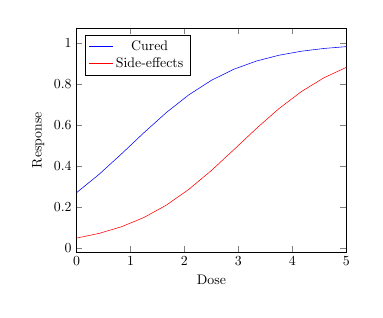
\begin{tikzpicture}[scale=0.5]
          \begin{axis}[xmin=0,xmax=5, xlabel={Dose}, ylabel={Response}, legend pos=north west]
            % use TeX as calculator:
            \addplot[color=blue] {1/(1 + e^(1-x))};
            \addplot[color=red] {1/(1 + e^(3-x))};
            \legend{Cured, Side-effects}
          \end{axis}
        \end{tikzpicture}
        \caption{Dose-response curve.}
        \label{fig:dose-response}
      \end{subfigure}
      \hspace{2em}
      \begin{subfigure}{\fwidth}
        \centering
        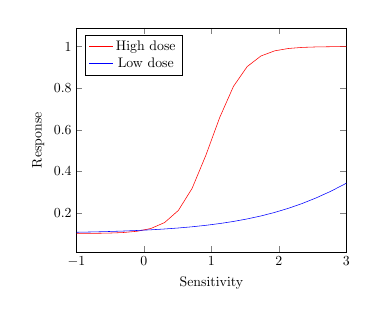
\begin{tikzpicture}[scale=0.5]
          \begin{axis}[xmin=-1,xmax=3, xlabel={Sensitivity}, ylabel={Response}, samples=50, legend pos=north west ]
            % use TeX as calculator:
            \addplot[color=red] {0.1 + 0.9*e^(4*(x-1))/(1+e^(4*(x-1)))};
            \addplot[color=blue] {0.1 + 0.9*e^(x-4)/(1+e^(x-4))};
            \legend{High dose, Low dose}
          \end{axis}
        \end{tikzpicture}
        \caption{Response sensitivity}
        \label{fig:dose-sensitivity}
      \end{subfigure}
      \caption{Investigating the response of the population to various doses of the drug.}
    \end{figure}
    \only<article>{
      We can ask ourselves two different questions about the effect of population effect aspirin on headaches.
    }
    \begin{itemize}
    \item Is aspirin an effective cure for headaches?
    \item Does having a headache lead to aspirin-taking?
    \end{itemize}
  \end{example}
  \only<article>{To examine the effect of aspirin on the population, we can look at the dose-response curve in Figure~\ref{fig:dose-response}. We first have to define what it means to be 'cured'. We also need to define possible side-effects. We can then measure how increased doses of aspirin lead to different outcomes. If the experiment has been properly conducted, this dose-response curve suggests that aspirin does have an effect in curing headaches, though it also has some side-effects. However, not all individuals are the same. Let us assume each person has a different \emph{sensitivity} to aspirin, so that some individuals responds better to treatment, especially at high doses, and some do not respond very much at all, as shown in Figure~\ref{fig:dose-sensitivity}}

\end{frame}
\begin{frame}
  \only<article>{For individuals, the first question is,  what is the possible effect of our actions? This is called the \emph{effect of causes}. The second question is, what was the reason for something happening? That is called the \emph{cause of effects?} }
  \begin{example}[Individual effects]
    \begin{figure}[H]
      \centering
      \begin{subfigure}{\fwidth}
        \includegraphics[width=\fwidth]{../figures/aspirin}
      \end{subfigure}
      \begin{subfigure}{\fwidth}
        \includegraphics[width=\fwidth]{../figures/450px-Migraine.jpg}
      \end{subfigure}
    \end{figure}
    \only<article>{
      We can ask ourselves two different questions about the individual effect of aspirin on headaches.
    }
    \begin{itemize}
    \item Effects of \alert{Causes}: Will \alert{my} headache pass \alert{if I take} an aspirin?
    \item \alert{Causes} of Effects: Would \alert{my} headache have passed if I had \alert{not taken} an aspirin?
    \end{itemize}
  \end{example}
  \only<article>{In order to be able to meaningfully talk about effects and causes we must also introduce decisions. Formally, there is nothing different in the decisions in this section and those introduced in Section~\ref{sec:decision-problems}. However, in this case we will try and use decisions to model outside interventions in a ``natural'' system, whereby a \emph{null} decision means that we do not intervene.}
\end{frame}

\begin{frame}
  \frametitle{Overview}
  \begin{block}{Inferring causal models}
    We can distinguish different \alert{models} from observational or experimental data.
  \end{block}

  \begin{block}{Inferring individual effects}
    The effect of possible intervention on an individual is not generally determinable. We usually require strong assumptions.
  \end{block}
  
  \begin{block}{Decision-theoretic view}
    There are many competing approaches to causality. We will remain within the decision-theoretic framework, which allows us to crisply define both our knowledge and assumptions.
  \end{block}
\end{frame}

\begin{frame}
  \frametitle{What causes what?}
  \begin{example}
    \begin{figure}[H]
      \centering
      \begin{subfigure}{\fwidth}
        \centering
        \begin{tikzpicture}
          \node[RV, hidden] at (0,1) (p) {$\param$};
          \node[RV] at (-1,0) (x1) {$a_t$};
          \node[RV] at (1,0) (x2) {$x_t$};
          \draw[->] (p) -- (x1);
          \draw[->] (p) -- (x2);
          \draw[->] (x1) -- (x2);
        \end{tikzpicture}
        \caption{Independence of $a_t$.}
      \end{subfigure}
      \begin{subfigure}{\fwidth}
        \centering
        \begin{tikzpicture}
          \node[RV, hidden] at (0,1) (p) {$\param$};
          \node[RV] at (-1,0) (x1) {$a_{t}$};
          \node[RV] at (1,0) (x2) {$x_{t}$};
          \draw[->] (p) -- (x1);
          \draw[->] (p) -- (x2);
          \draw[->] (x2) -- (x1);
        \end{tikzpicture}
        \caption{Independence of $x_t$.}
      \end{subfigure}
    \end{figure}
    Suppose we have data $x_{t}, a_{t}$ where
    \begin{itemize}
    \item $x_{t}$: lung cancer
    \item $a_{t}$: smoking
    \end{itemize}
    Does smoking cause lung cancer or does lung cancer make people smoke? Can we compare the two models above to determine it?
  \end{example}
  \only<article>{The answer is no. Let us consider two different parametrisations of the distribution. One in which $a_t$ generates $x_t$, and the converse, for any given parameter value $\param$, as given below:}
  \uncover<2>{
    \[
    P_\param(D) =
    \prod_t P_\param(x_t, a_t)
    = 
    \prod_t P_{\param'}(x_t \mid a_t) P_{\param'}(a_t)
    = 
    \prod_t P_{\param''}(a_t \mid x_t) P_{\param''}(x_t).
    \]
  }
  \only<article>{In particular, for any parametrisation $\param$ of the joint distribution, there exists a $\param'$ and $\param''$ giving the same probabilities for all $x_t, a_t$. For the example above, we can look at Bernoulli distributions for both variables so that $P_\param(x_t = x, a_t = a) = \param_{x,a}$. Then
    \begin{align*}
      \param'_a &= \sum_x \param_{x,a},
      &
        \param'_{x|a} &= \param_{x,a} / \param'_a
      \\
      \param''_x &= \sum_a \param_{x,a},
      &
        \param'_{a|x} &= \param_{x,a} / \param''_x.
    \end{align*}
    This means we can define prior distributions $\bel, \bel', \bel''$ in these three parameter spaces that give exactly the same results, e.g. by modelling each parameter as an independent Beta distribution. So, clearly simply looking at a simple graphical model does not let us answer this question.}
\end{frame}

\subsection{Decision diagrams}
\only<article>{
  However, graphical models \alert{can} be extended  to model causal relations. In particular, we can use \emph{decision diagrams}\footnote{Otherwise called influence diagrams}, which include not only random variables, but also \emph{decision} variables, denoted with squares, as well as utility variables, denoted via diamonds. In the following examples, we assume there are some underlying distributions specified by parameters $\param$, which we include in the diagrams for clarity. Even though it may seem intuitively sensible to suppose it, the arrow directions in the diagrams \emph{do not} indicate direct causes. The only important thing for determining whether some variable influences another is whether or not there is independence between the corresponding decision and random variables.}
\begin{frame}
  \begin{figure}[H]
    \centering
    \begin{tikzpicture}
      \node[RV, hidden] at (-1,1) (p) {$\param$};
      \node[RV] at (0,0) (x) {$x_t$};
      \node[RV] at (1,1) (y) {$y_t$};
      \only<1,2>{
        \node[select] at (2,0) (a) {$a_t$};
      }
      \only<3->{
        \node[RV] at (2,0) (a) {$a_t$};
      }
      \draw[->] (x)--(y);
      \draw[->] (x)--(a);
      \draw[->] (a)--(y);
      \draw[->] (p) to (x);
      \draw[->] (p)--(y);
      \onslide<3->{
        \node[select] at (4,0) (pol) {$\pol$};
        \draw[->] (pol)--(a);
      }
      \onslide<2->{
        \node[utility] at (3,1) (u) {$\util$};
        \draw[->] (a)--(u);
        \draw[->] (y)--(u);
      }
    \end{tikzpicture}
    \caption{A typical decision diagram where $x_t$: individual information, $y_t$: individual result, $a_t$: action, $\pol$: policy}
    \label{fig:decision-diagram}
    \index{policy!intervention}
  \end{figure}
  \only<3>{
    \begin{example}[Taking an aspirin]
      \only<article>{The diagram in Figure~\ref{fig:decision-diagram} does not completely specify the decision problem. For aspirin taking, we can define the following variables:}
      \begin{itemize}
      \item Individual $t$
      \item Individual information $x_t$
      \item $a_t  = 1$ if $t$ takes an aspirin, and $0$ otherwise.
      \item $y_t = 1$ if the headache is cured in 30 minutes, $0$ otherwise.
      \item $\pol$: intervention policy.\index{policy!intervention}
      \end{itemize}
    \end{example}
  }
  \only<4>{
    \begin{example}[A recommendation system]
      \only<article>{Consider the example of a recommendation system, where we have data of the form $(x_t, a_t, y_t)$. The performance of the recommendation system depends not only on the parameter $\param$, but also on the chosen policy $\pol$. }
      \begin{itemize}
      \item $x_t$: User information (random variable)
      \item $a_t$: System action (random variable)
      \item $y_t$: Click (random varaible)
      \item $\pol$: recommendation policy (decision variable).\index{policy!recommendation}
      \end{itemize}
    \end{example}
  }
  \only<article>{In both cases, there are some questions we can ask using the underlying model. The dependency structure is not enough to know \emph{a priori} whether we can obtain meaningful answers. This depends on the specific assumptions we make about the model.}
\end{frame}

\begin{frame}
  \frametitle{Conditional distributions and decision variables.}
  \only<article>{We begin with a parenthesis on conditional distributions. We normally define the conditional distribution of $A$ given $B$ under a probability measure $P$ as:}
  \[
  P(A \mid B) \defn \frac{P(A \cap B)}{P(B)}.
  \]
  \only<article>{However, decision variables are outside the scope of this probability measure, and yet we need to define conditional distributions using them. }
  \begin{block}{The conditional distribution of decisions}
    \only<article>{If $\pol \in \Pol$ is a decision variable, we represent the conditional distribution of any random variable $a$ given $\pol$ simply as a collection of probability measures $\cset{\pol(a)}{\pol \in \Pol}$, one for each possible value $\pol$. The following notations will be equivalent:}
    \[
    \pol(a) \equiv \Pr^\pol(a) \equiv \Pr(a \mid \pol).
    \]
    \only<article>{The reader should note that the standard definition of a conditional distribution also $P(A \mid B)$ creates a collection of distributions on $A$, with elements $P_B(A)$. However, it also specifies a rule for doing so from the complete distribution $P$. 

      If the random variables $a$ also depends on some probability law $P_\param$, then it will be convenient to use the notation
    }
    \[
    \Pr_\param^\pol(a) \equiv \Pr(a \mid \param, \pol).
    \]
  \end{block}
\end{frame}
\subsection{Common structural assumptions}
\only<article>{
  In order to be clear about what constitutes an observation by the experimenter and what is a decision, we must clearly separate random variables from decision variables. The individual actions may be random variables, but they will depend on decisions taken. As we will see later, this is useful for modelling interventions.}

\begin{frame}
  \frametitle{Basic causal structures}
  \only<article>{Directed graphical models are not sufficient to determine causality by themselves, as they only determine correlations between random variables. If we have decision variables, however, we can always determine whether or not our decisions influence outcomes.}
  \begin{block}{Non-cause}
    \begin{figure}[H]
      \centering
      \begin{tikzpicture}
        \node[select] at (0,0) (p) {$\pol$};
        \node[RV] at (1,0) (a) {$a_t$};
        \node[RV] at (2,0) (y) {$y_t$};
        \draw[->] (p) to (a);
        \draw[->] (y) to (a);
        \uncover<2>{
          \node[RV, hidden] at (1,1) (param) {$\param$};
          \draw[->] (param) to (y);
        }
      \end{tikzpicture}
      \caption{$\pol$ does not cause $y$}
      \label{fig:non-cause}
    \end{figure}
    \only<article>{In the diagram above, we see that $y_t \indep \pol$.}
  \end{block}
  \only<article>{
    \begin{example}
      Consider the model
      \begin{align*}
        y_t &\sim \Normal(0,1)\\
        a_t \mid y_t, \pol &\sim \Normal(y_t + \pol, 1)
      \end{align*}
      \begin{figure}[H]
        \centering
        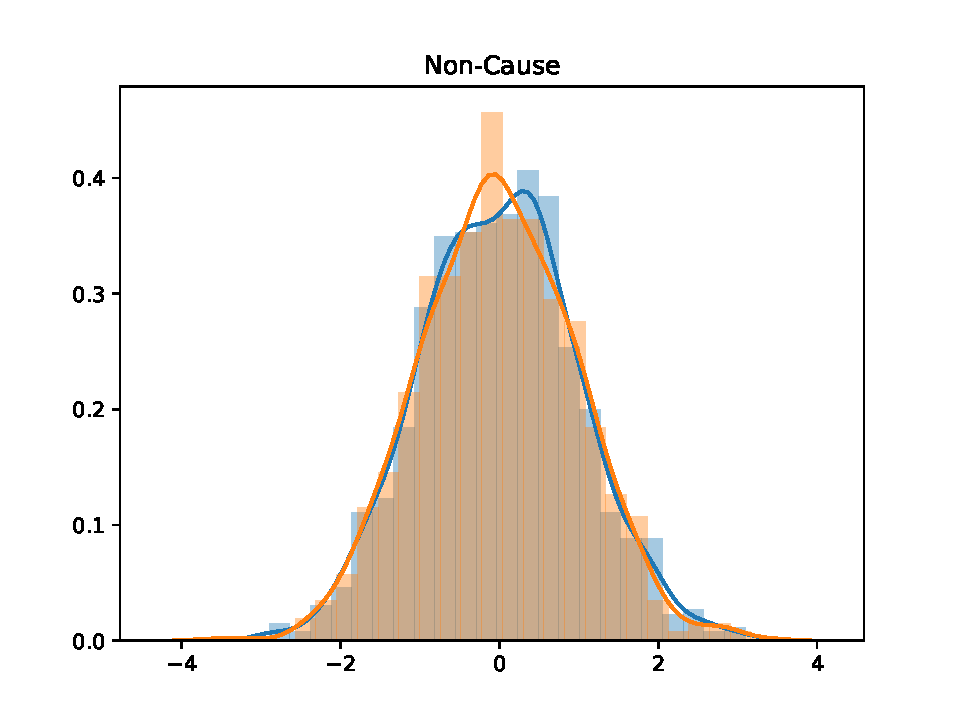
\includegraphics[width=0.5\textwidth]{../src/causality/non-cause}
        \caption{$\Pr^\pol(y_t)$ for $\pol \in \{-1, 1\}$ when $\pol$ is not a cause for $y_t$}
        \label{fig:non-cause-dist}
      \end{figure}
      In this example, we see tht $y_t$ is independent of the policy
      $\pol$.  However, $y_t$ is not independent of the action taken, as the action depends on $y_t$ directly. The correlation between $y, a$ is shown in Figure~\ref{fig:a-y-correlation:non-cause}.
    \end{example}
  }
  
  \begin{block}{No confounding}
    \only<article>{Confounding is a term that indicates the existence of latent variables that create dependencies between $y_t, \pol, a_t$. We are sure that there is no confounding whenever $y_t \indep \pol \mid a_t$, as captured by the diagram in Figure~\ref{fig:no-confounding}. In this case $\pol$ is a direct cause for $y_t$ through $a_t$.}
    \begin{figure}[H]
      \centering
      \begin{tikzpicture}
        \node[select] at (0,0) (p) {$\pol$};
        \node[RV] at (1,0) (a) {$a_t$};
        \node[RV] at (2,0) (y) {$y_t$};
        \draw[->] (p) to (a);
        \draw[->] (a) to (y);
        \uncover<2>{
          \node[RV, hidden] at (1,1) (param) {$\param$};
          \draw[->] (param) to (y);
        }
      \end{tikzpicture}
      \caption{No confounding: $\pol$ causes $y_t$}
      \label{fig:no-confounding}
    \end{figure}
  \end{block}

  \only<article>{
    \begin{example}
      Consider the model
      \begin{align*}
        a_t &\sim \Normal(\pol,1)\\
        y_t \mid a_t, \pol &\sim \Normal(a_t, 1)
      \end{align*}
      \begin{figure}[H]
        \centering
        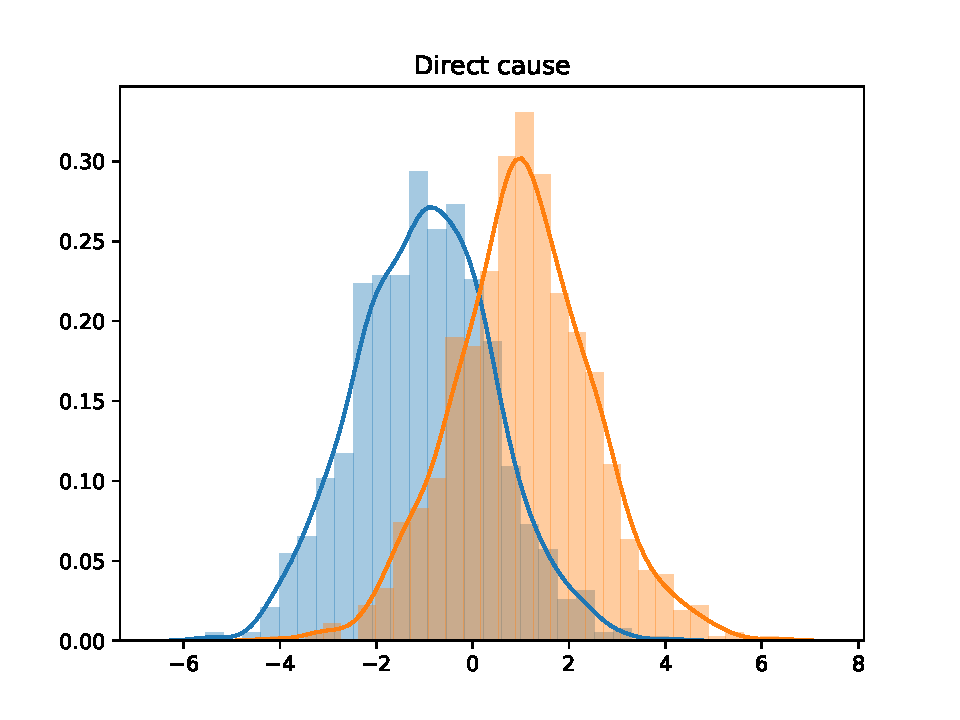
\includegraphics[width=0.5\textwidth]{../src/causality/direct-cause}
        \caption{$\Pr^\pol(y_t)$ for $\pol \in \{-1, 1\}$ when $\pol$ is a direct cause for $y_t$}
        \label{fig:non-cause-dist}
      \end{figure}
      \only<article>{We can see how the distribution of $y_t$ changes when $\pol$ changes in Figure~\ref{fig:non-cause-dist}. In this case there is also a correlation between $a_t, y_t$ as seen in Figure~\ref{fig:a-y-correlation}.}
    \end{example}
  }

  \only<article>{
    \begin{figure}[H]
      \centering
      \begin{subfigure}{0.45\textwidth}
        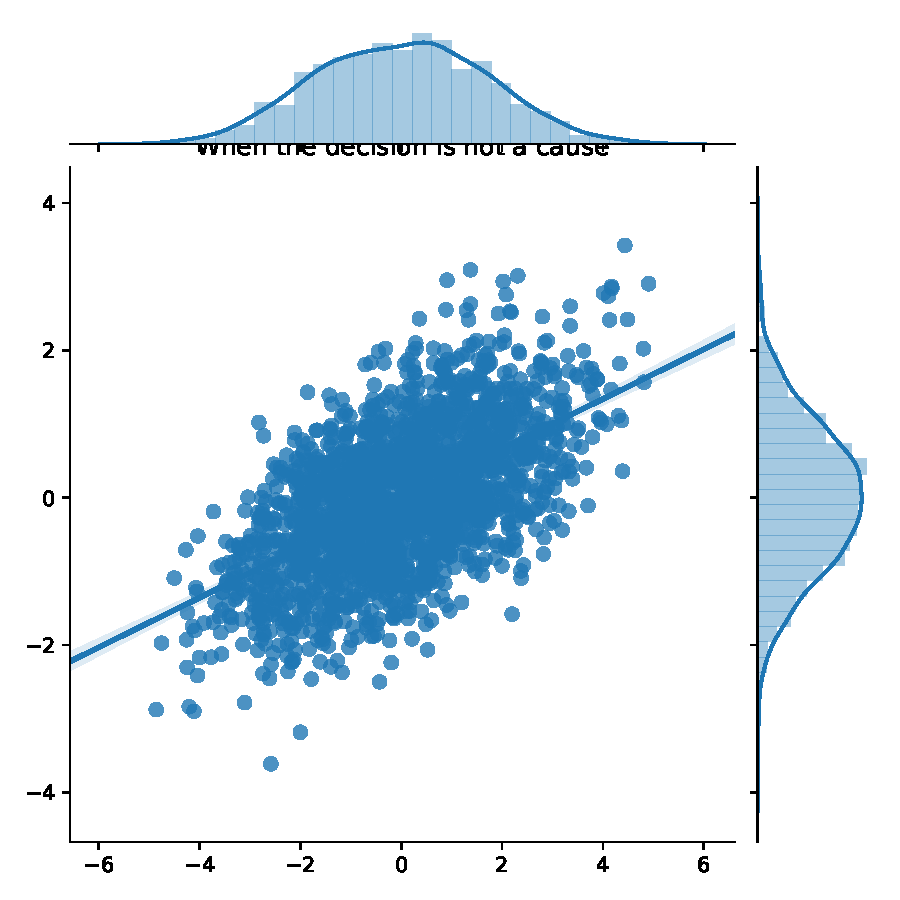
\includegraphics[width=0.9\textwidth]{../src/causality/a-y-non-cause}
        \caption{Non-cause}
        \label{fig:a-y-correlation:non-cause}
      \end{subfigure}
      \hspace{1em}
      \begin{subfigure}{0.45\textwidth}
        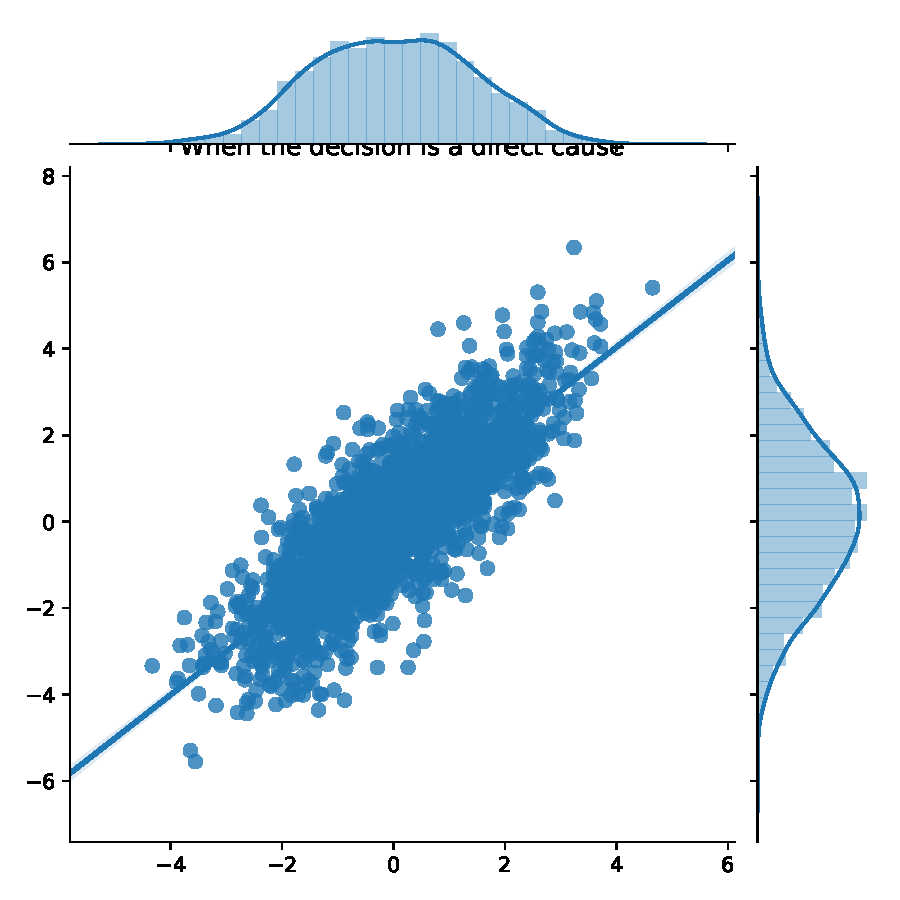
\includegraphics[width=0.9\textwidth]{../src/causality/a-y-direct-cause}
        \caption{Cause}
        \label{fig:a-y-correlation:cause}
      \end{subfigure}
      \caption{Correlation between $a_t$ and $y_t$}
      \label{fig:a-y-correlation}
    \end{figure}
  }
\end{frame}
\begin{frame}
  \frametitle{Covariates}
  \begin{block}{Sufficient covariate}
    \only<article>{Sometimes the variable of interest is not conditionally independent of the treatment, unless there exists a \emph{sufficient covariate} $x_t$ such that
      $y_t \indep \pol \mid a_t, x_t$. If $x_t$ is not observed, then it is sometimes called a confounder.}
    \begin{figure}[H]
      \centering
      \begin{tikzpicture}
        \node[select] at (0,0) (p) {$\pol$};
        \node[RV] at (1,0) (a) {$a_t$};
        \node[RV] at (2,0) (y) {$y_t$};
        \node[RV] at (2,1) (x) {$x_t$};
        \draw[->] (p) to (a);
        \draw[->] (a) to (y);
        \draw[->] (x) to (a);
        \draw[->] (x) to (y);
        \uncover<2>{
          \node[RV, hidden] at (3,1) (param) {$\param$};
          \draw[->] (param) to (x);
          \draw[->] (param) to (y);
        }
      \end{tikzpicture}
      \caption{Sufficient covariate $x_t$}
      \label{fig:sufficient-covariate}
    \end{figure}
  \end{block}

  \only<article>{
    \begin{example}
      Consider the model
      \begin{align*}
        x_t &\sim \Normal(0, 1)\\
        a_t &\sim \Normal(x_t + \pol, 1)\\
        y_t \mid a_t, \pol &\sim \Normal(x_t + a_t, 1),
      \end{align*}
      \only<article>{Here $x_t$ influences the outcome $y_t$, but also directly influences $a_t$ through the policy $\pol$. As we can see in Figure~\ref{fig:non-cause-dist}, the policy then has an influence on $y_t$}
      \begin{figure}[H]
        \centering
        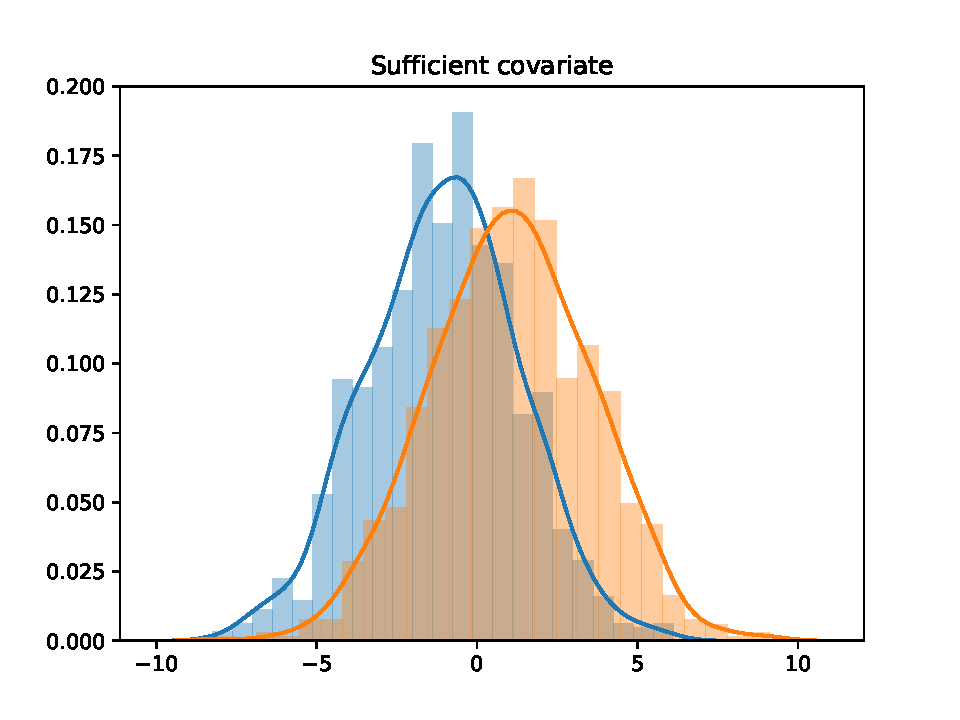
\includegraphics[width=0.5\textwidth]{../src/causality/sufficient}
        \caption{$\Pr^\pol(y_t)$ for $\pol \in \{-1, 1\}$ when $\pol$ is a direct cause for $y_t$}
        \label{fig:sufficient-covariate-dist}
      \end{figure}
    \end{example}
  }


  \begin{block}{Instrumental variables and confounders}
    \only<article>{If the sufficient covariate $x_t$ is not observed, we may still have another variable available, $z_t$, on the basis of which we make our decisions. This is called an \emph{instrumental variable.} \index{instrument@see{variable!instrumental}}\index{variable!instrumental}. More formally, $z_t$ is an instrumental variable with respect to $y_t$ since the latent variables on which $y_t$ depends satisfy $x_t, \param \indep \pol$ and the outcome variable is independent of the policy given the action and the two latent variables: $y \indep pol \mid a_t, x_t, \param$.
      
      In this case $z_t$ and $x_t$ are dependent, but the effect of the treatment depends on $x_t$ directly. As $x_t$ is a latent covariate, it can be called a \emph{confounder.} \index{confounder}}
    \begin{figure}[H]
      \centering
      \begin{tikzpicture}
        \node[select] at (0,0) (p) {$\pol$};
        \node[RV] at (1,0) (a) {$a_t$};
        \node[RV] at (2,0) (y) {$y_t$};
        \node[RV, hidden] at (2,1) (x) {$x_t$};
        \node[RV] at (1,1) (z) {$z_t$};
        \draw[->] (p) to (a);
        \draw[->] (a) to (y);
        \draw[->] (x) to (y);
        \draw[->] (x) to (z);
        \draw[->] (z) to (a);
        \uncover<2>{
          \node[RV, hidden] at (3,1) (param) {$\param$};
          \draw[->] (param) to (x);
          \draw[->] (param) to (y);
          \draw[bend right=45,->] (param) to (z);
        }
      \end{tikzpicture}
      \caption{Instrumental variable $z_t$}
      \label{fig:instrumental-variable}
    \end{figure}
  \end{block}

  \only<article>{
    \begin{example}
      Consider the model
      \begin{align*}
        x_t &\sim \Normal(0, 1)\\
        z_t &\sim \Normal(x_t, 1)\\
        a_t &\sim \Normal(z_t + \pol, 1)\\
        y_t \mid a_t, \pol &\sim \Normal(x_t + a_t, 1)
      \end{align*}
      \only<article>{In this scenario, $x_t$ directly influences the outcome $y_t$, but is not observed.\footnote{Hence, it can be called a confounder.}}
      \begin{figure}[H]
        \centering
        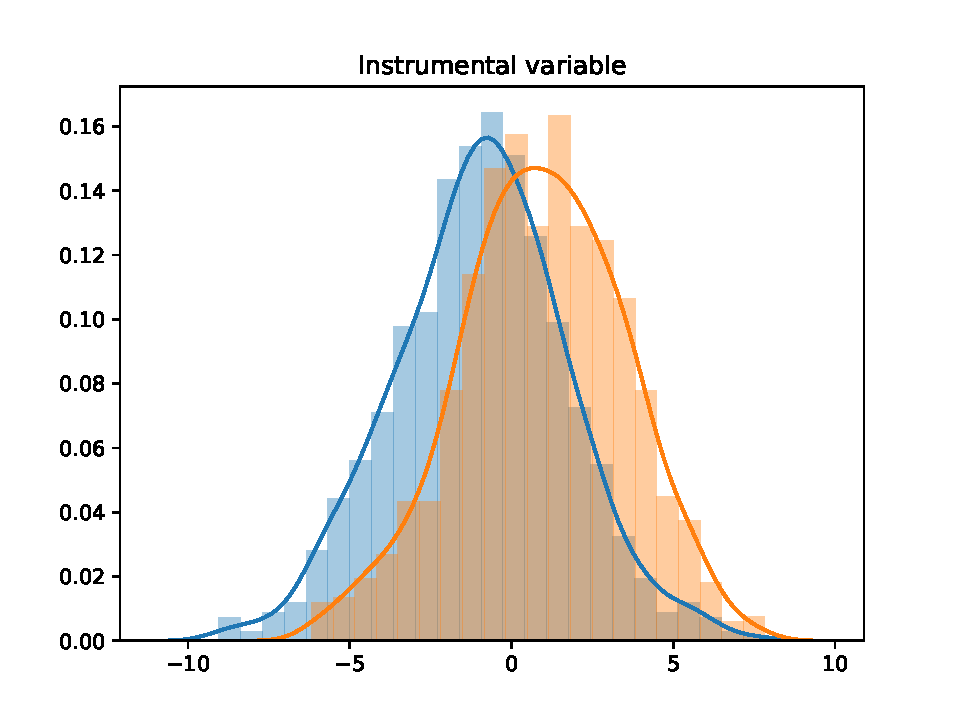
\includegraphics[width=0.5\textwidth]{../src/causality/instrumental}
        \caption{$\Pr^\pol(y_t)$ for $\pol \in \{-1, 1\}$ when $\pol$ is a direct cause for $y_t$}
        \label{fig:instrumental-dist}
      \end{figure}
    \end{example}
  }

  \only<article>{Finally, variables which are neither confounders, nor instrumental, are called nuisance variables. Typically these include the latent variables of the problem, and any other variable that is marginalised out.}
\end{frame}
  
\section{Interventions}
\only<article>{Interventions are of primary interest when we have a set of observational data, collected under a \emph{null} or \emph{default} policy $\pol_0$.  We then wish to intervene with some policy $\pol$ in order to maximise our utility function, or to simply try and estimate the exact relationships between variables.}
\begin{frame}
  \frametitle{Modelling interventions}
  \begin{itemize}
  \item Observational data $D$. \only<article>{This represents data we have collected from some previous regime. In order to be able to model the problem precisely, we must posit the existence of some default policy $\pol_0$ under which the data was collected.}
  \item Policy space $\Pol$. \only<article>{This must include $\pol_0$, as well as any other policies that the decision maker may be able to choose in the future.} 
  \end{itemize}
  \begin{block}{Default policy}
    \index{policy!default}
    The space of policies $\Pol$ includes a \alert{default policy} $\pol_0$, under which the data was collected. \only<article>{The policy $\pol_0$ might already be known, if for example the data was collected with a specific algorithm. However, frequently $\pol_0$ is not given, and must also be inferred from the data. In that case, it can be seen as an additional parameter, complementary to $\param$.}
  \end{block}
  \begin{block}{Intervention policies}
    \index{policy!intervention}
    Except $\pol_0$, policies $\pol \in \Pol$ represent different interventions specifying a distribution $\pol(a_t \mid x_t)$.
    \begin{itemize}
    \item Direct interventions. \only<article>{The simplest scenario is when we are able to choose a $\pol$ for which we know $\pol(a_t \mid x_t)$. This counts as a direct intervention, as we can specify any distribution of actions allowed in $\Pol$. If $\Pol$ includes all conditional distributions, we can select an arbitrary action for every individual. This assumption is plausible for algorithmic decision making such as recommendation systems, but implausible when the actions are taken by another agent, such as a human.}
    \item Indirect interventions and non-compliance. \only<article>{In this scenario we assume that, while we are free to choose policies from $\Pol$, we do not know what distribution $\pol(a_t \mid x_t)$ each policy specifies. In algorithmic decision making, this occurs whenever $\pol$ represents hyperparameters and algorithms for which we have insufficient information. Then policies must be evaluated through some type of black-box (e.g. A/B) testing. When the actions are taken by (human) agents, the policy implies making a recommendation, which may not be followed by the agent. If we denote the recommendation by $v_t$, then we can write $\pol(a_t \mid x_t) = \sum_{z_t} \pol(a_t \mid z_t, x_t) \pol(z_t \mid x_t)$. In this scenario we can freely specify $\pol(z_t \mid x_t)$, but $\pol(a_t \mid z_t, x_t)$ must be estimated. For that reason, it is usually simpler to simply marginalise out $a_t$. But perhaps the simplest approach is to consider non-compliance as a confounder $x_t$, and $z_t$ as an instrumental variable. }
    \end{itemize}
  \end{block}
\end{frame}
\begin{frame}
  \begin{example}[Weight loss]
    \only<article>{Consider weight loss. We can collect observational data from a population of overweight adults over a year. We can imagine that $x$ represents the weight and vital statistics of an individual and $y$ their change in weight after a year. We may also observe their individual actions $a$, such as whether or not they are following a particular diet or exercise regime. Under the default policy $\pol_0$, their actions are determined only the individuals. Consider an alternative policy $\pol$, which prescribes diet and exercise regimes. Due to non-compliance, actual actions taken by individuals may differ from prescribed actions. In addition, actions might not be observed.}
    \only<presentation>{
      \only<1>{
        \begin{figure}[H]
          \centering
                \begin{tikzpicture}
        \node[RV, hidden] at (0,1) (p) {$\param$};
        \node[RV] at (0,0) (x) {$x_t$};
        \node[RV] at (1,1) (y) {$y_t$};
        \node[RV] at (2,0) (a) {$a_t$};
        \draw[->] (p)--(x);
        \draw[->] (p)--(y);
        \draw[->] (x)--(y);
        \draw[->] (x)--(a);
        \draw[->] (a)--(y);
        \node[select] at (4,0) (p) {$\pol$};
        \draw[->] (p)--(a);
        \node[utility] at (3,1) (u) {$\util$};
        \draw[->] (a)--(u);
        \draw[->] (y)--(u);
      \end{tikzpicture}

%%% Local Variables:
%%% mode: latex
%%% TeX-master: "notes"
%%% End:

        \end{figure}
      }
    }
    \only<2>{
      \begin{figure}[H]
        \centering
        \begin{tikzpicture}
          \node[RV, hidden] at (0,1) (p) {$\param$};
          \node[RV] at (0,0) (z) {$z_t$};
          \node[RV, hidden] at (1,2) (x) {$x_t$};
          \node[RV] at (1,1) (y) {$y_t$};
          \node[RV] at (2,0) (a) {$a_t$};
          \draw[->] (p)--(z);
          \draw[->] (p)--(x);
          \draw[->] (p)--(y);
          \draw[->] (x)--(y);
          \draw[->] (z)--(y);
          \draw[->] (z)--(a);
          \draw[->] (a)--(y);
          \node[select] at (4,0) (p) {$\pol$};
          \draw[->] (p)--(a);
          \node[utility] at (3,1) (u) {$\util$};
          \draw[->] (a)--(u);
          \draw[->] (y)--(u);
        \end{tikzpicture}
        \caption{Model of non-compliance as a confounder.}
        \label{fig:non-compliance}
      \end{figure}
    }
  \end{example}
\end{frame}  


\section{Policy evaluation and optimisation}
\index{policy!evaluation}
\begin{frame}
  \frametitle{The value of an observed policy}
  \only<presentation>{
    \begin{figure}[H]
      \centering
            \begin{tikzpicture}
        \node[RV, hidden] at (0,1) (p) {$\param$};
        \node[RV] at (0,0) (x) {$x_t$};
        \node[RV] at (1,1) (y) {$y_t$};
        \node[RV] at (2,0) (a) {$a_t$};
        \draw[->] (p)--(x);
        \draw[->] (p)--(y);
        \draw[->] (x)--(y);
        \draw[->] (x)--(a);
        \draw[->] (a)--(y);
        \node[select] at (4,0) (p) {$\pol$};
        \draw[->] (p)--(a);
        \node[utility] at (3,1) (u) {$\util$};
        \draw[->] (a)--(u);
        \draw[->] (y)--(u);
      \end{tikzpicture}

%%% Local Variables:
%%% mode: latex
%%% TeX-master: "notes"
%%% End:

      \caption{Basic decision diagram}
    \end{figure}
  }
  \only<article>{
    In this section, we will focus on the general model of Figure~\ref{fig:decision-diagram}.
    If we have data $D = \cset{(x_t, a_t, y_t)}{t \in [T]}$ generated from some policy $\pol_0$, we can always infer the average quality of each action $a$ under that policy.}
  \only<2>{
    \begin{align}
      \label{eq:observed-expected-utility}
      \hat{\E}_D(U \mid a) 
      &\defn
        \frac{1}{|\cset{t}{a_t = a}|}
        \sum_{t: a_t = a}
        U(a_t, y_t)\\
      &\approx
        \E^{\pol_0}_\param (U \mid a)
      & (a_t, y_t) & \sim \Pr_\param^{\pol_0}.
    \end{align}
  }
  \only<article>{
    Can we calculate the value of another policy? As we have seen from Simpson's paradox\index{Simpson's paradox}, it is folly to simply select
  }
  \[
  \hat{a}^*_D \in \argmax_a \hat{\E}_D(U \mid a),
  \]
  \only<article>{
    as the action also depends on the observations $x$ through the policy.
    To clarify this, let us look again at the model shown in Figure~\ref{fig:decision-diagram}.
  }
\end{frame}
\begin{frame}

  \begin{align*}
    x_t \mid \param &\sim P_\param(x)\\
    y_t \mid \param, x_t, a_t &\sim P_\param(y \mid x_t, a_t)\\
    a_t \mid x_t, \pol &\sim \pol(a \mid x_t).
  \end{align*}
  \only<article>{
    Assume that $x \in \CX$, a continuous space, but $y \in \CY$ is discrete. In this scenario, then the value of an action under a policy $\pol$ is nonsensical, as it does not really depend on the policy itself:
    \begin{align*}
      \E^\pol_\param(\util \mid a)
      &=
        \int_\CX \dd P_\param(x)
        \sum_{y \in \CY} P_\param(y \mid x, a) \util(a, y).
    \end{align*}
    We see that there is a clear dependence on the distribution of $x$, and there is no dependence on the policy any more. In fact, equation above only tells us the expected utility we'd get if we always chose the same action $a$. But what is the optimal policy? First, we have to define the value of a policy.}
  \begin{block}{The value of a policy}
    \begin{align*}
      \E^\pol_\param(\util)
      &=
        \int_\CX \dd P_\param(x)
        \sum_{a \in \CA}  \pol(a \mid x)  \sum_{y \in \CY} P_\param(y \mid x, a) \util(a, y)
    \end{align*}
  \end{block}
  The optimal policy under a known parameter $\param$ is given simply by
  \begin{align*}
    \max_{\pol \in \Pol} \E^\pol_\param(\util),
  \end{align*}
  where $\Pol$ is the set of allowed policies. 
\end{frame}

\begin{frame}
  \frametitle{Monte-Carlo estimation}
  \only<article>{The simplest method to estimate the value of an alternative policy is to use Monte-Carlo estimation and importance sampling. However, this estimate can have a very high variance if the alternative policy is very different from the original policy.}
  \begin{block}{Importance sampling\footnote{Also known as Propensity Scoring}}
    We can obtain an unbiased estimate of the utility in a model-free manner through importance sampling:
    \only<presentation>{
      \begin{align*}
        \E^\pol_\param(\util)
        &=
          \int_\CX \dd P_\param(x)
          \sum_a
          \E_\param(\util \mid a, x)
          \pol(a \mid x)\\
        &\approx
          \frac{1}{T}
          \sum_{t=1}^T
          \util_t 
          \frac{\pol(a_t \mid x_t)}{\pol_0(a_t \mid x_t)}.
      \end{align*}
    }

    \only<article>{
      \begin{align*}
        \E^\pol_\param(\util)
        &=
          \int_\CX \dd P_\param(x)
          \sum_a
          \E_\param(\util \mid a, x)
          \pol(a \mid x)\\
        &\approx
          \frac{1}{T}
          \sum_a \sum_t
          \E_\param(\util \mid a, x_t)
          \pol(a \mid x_t), & x_t & \sim P_\param(x)\\
        &=
          \frac{1}{T}
          \sum_t \sum_a
          \E_\param(\util \mid a, x_t)
          \frac{\pol(a \mid x_t)}{\pol_0(a \mid x_t)} \pol_0(a \mid x_t)\\
        &\approx
          \frac{1}{T}
          \sum_{t=1}^T
          \util_t 
          \frac{\pol(a_t \mid x_t)}{\pol_0(a_t \mid x_t)},
        & a_t \mid x_t \sim & \pol_0, \quad U_t \mid x_t, a_t \sim P_\param(U_t \mid x_t, a_t)
      \end{align*}
    }
  \end{block}
\end{frame}

\begin{frame}
  \frametitle{Bayesian estimation}
  \only<article>{Unforunately this method has high variance.}
  If we $\pol_0$ is given, we can calculate the utility of any policy to whatever degree of accuracy we wish. \only<article>{We begin with a prior $\bel$ on $\Param$ and obtain the following, assuming the policy $\pol_0$ is stationary.}
  \begin{align*}
    \bel(\param \mid D, \pol_0) &\propto \prod_t \Pr^{\pol_0}_\param(x_t, y_t, a_t)\\
    \E_\bel^\pol(\util \mid D) &= \int_\Param \E_\param^\pol(\util) \dd \bel(\param \mid D)\\
                                &= \int_\Param 
                                  \int_\CX \dd P_\param(x)
                                  \sum_{t=1}^T
                                  \sum_a
                                  \E_\param(\util \mid a, x)
                                  \pol(a \mid x)
                                  \dd \bel(\param \mid D).
  \end{align*}
\end{frame}


\begin{frame}
  \frametitle{Causal inference and policy optimisation}
  \index{policy!optimisation}
  \only<article>{Causal inference requires building a complete model for the effect of both the model parameter $\param$, representing nature, and the policy $\pol$, representing the decision maker. This means that we have to be explicit about the dependencies of random variables on the model and the policy.}
  \only<1>{
    \begin{example}
      \begin{figure}[H]
        \centering
        \begin{tikzpicture}
          \node[RV, hidden] at (0,0) (p) {$\param$};
          \node[RV] at (1,0) (y) {$y_t$};
          \node[RV] at (2,0) (a) {$a_t$};
          \node[select] at (3,0) (pol) {$\pol$};
          \draw[->] (pol)--(a);
          \draw[->] (p)--(y);
          \draw[->] (a)--(y);
          \node[utility] at (2,1) (u) {$\util$};
          \draw[->] (a)--(u);
          \draw[->] (y)--(u);
        \end{tikzpicture}
        \caption{Simple decision problem.}
      \end{figure}
      Let $a_t, y_t \in \{0,1\}$, $\param \in [0,1]^2$ and
      \[
      y_t \mid a_t = a \sim \Bernoulli(\param_a)
      \]
      Then, by estimating $\param$, we can predict the effect of any action.
      \only<article>{
        How can we estimate $\param$ from historical data? We simply have to select the right parameter value.
        Simply put, each choice of $a$ corresponds to one part of the parameter vector. This means that the maximum likelihood estimate 
        \[
        \hat{\param}_a \defn \frac{1}{|\cset{t}{a_t = a}|} \sum_{\cset{t}{a_t = a}} y_t
        \]
        is valid. We can also consider a product-Beta prior $\BetaDist(\alpha^0_a, \beta^0_b)$ for each one of the Bernoulli parameters, so that the posterior after $t$ observations is
        \[
        \alpha^t_a = \alpha^0_a + \sum_{\cset{t}{a_t = a}} y_t, \qquad
        \beta^t_a = \beta^0_a + \sum_{\cset{t}{a_t = a}} (1 - y_t).
        \]
        How can we optimise the policy? 
        Let us parametrise our policy with $\pol(a_t = 1) = w$.

        For a fixed $\param$, the value of the policy is
        \[
        \E^\pol_\param \util = 
        \param_1 w + \param_0 (1 - w)
        \]
        The gradient with respect to w is 
        \[
        \nabla \E^\pol_\param \util = 
        \param_1 - \param_0, 
        \]
        so we can use the update
        \[
        w^{(n+1)} = w^{(n)} + \delta^{(n)} \param_1 - \param_0.
        \]
        \alert{However}, $w \in [0,1]$, which means our optimisation must be constrained. Then we obtain that
        $w = 1$ if $\param_1 > \param_0$ and $0$ otherwise.

        When $\param$ is not known, we can use stochastic gradient descent.
        \index{gradient ascent!stochastic}
        \[
        \nabla \E^\pol_\bel \util = 
        \int_\Param [\nabla \E^\pol_\param \util] \dd \bel(\param)
        \]
        to obtain:
        \[
        w^{(n+1)} = w^{(n)} + \delta^{(n)} \param^{(n)}_1 - \param^{(n)}_0.
        \]
        where $\param^{(n)} \sim \bel$.
      }

    \end{example}
  }

  \only<2>{
    \begin{example}
      \begin{figure}[H]
        \centering
        \begin{tikzpicture}
          \node[RV, hidden] at (0,0) (p) {$\param$};
          \node[RV] at (1,0) (y) {$y_t$};
          \node[RV] at (2,0) (a) {$a_t$};
          \node[select] at (3,0) (pol) {$\pol$};
          \draw[->] (pol)--(a);
          \draw[->] (p)--(y);
          \draw[->] (a)--(y);
          \node[utility] at (2,1) (u) {$\util$};
          \draw[->] (a)--(u);
          \draw[->] (y)--(u);
          \node[RV] at (1,-1) (x) {$x_t$};
          \draw[->] (x)--(a);
          \draw[->] (x)--(y);
          \draw[->] (p)--(x);
        \end{tikzpicture}
        \caption{Decision problem with covariates.}
      \end{figure}
      Let $a_t, x_t = \{0,1\}$, $y_t \in \Reals$, $\param \in \Reals^4$ and
      \[
      y_t \mid a_t = a, x_t = x \sim \Bernoulli(\param_{a,x})
      \]
      Then, by estimating $\param$, we can predict the effect of any action.
    \end{example}
  }


\end{frame}
\section{Individual effects and counterfactuals}

\only<article>{
  Counterfactual analysis is mainly about questions relative to individuals, and specifically about what the effects of alternative actions would have been in specific instances in the past. We will assume a decision-theoretic viewpoint throughout, in order to be as clear as possible and avoiding imprecise language.
}
\subsection{Disturbances and structural equation models}

\begin{frame}
  \only<article>{A structural equation model describes the random variables as deterministic functions of the decisions variables and the random exogenous disturbances. This allows us to separate the unobserved randomness from the known functional relationship between the other variables. Structurally, the model is essentially a variant of decision diagrams, as shown in Figure~\ref{fig:disturbance-model}.}
  \begin{figure}[H]
    \centering
    \begin{tikzpicture}
      \node[RV, hidden] at (-1,1) (p) {$\param$};
      \node[RV] at (0,0) (x) {$x_t$};
      \node[RV] at (1,1) (y) {$y_t$};
      \node[RV] at (2,0) (a) {$a_t$};
      \draw[->] (x)--(y);
      \draw[->] (x)--(a);
      \draw[->] (a)--(y);
      \draw[->] (p) to (x);
      \draw[->] (p)--(y);
      \node[select] at (4,0) (pol) {$\pol$};
      \draw[->] (pol)--(a);
      \node[utility] at (3,1) (u) {$\util$};
      \draw[->] (a)--(u);
      \draw[->] (y)--(u);
      \node[RV, hidden, above of=y]  (oy) {$\omega_{t,y}$};
      \node[RV, hidden, below of=x]  (ox) {$\omega_{t,x}$};
      \node[RV, hidden, below of=a]  (oa) {$\omega_{t,a}$};
      \draw[->] (ox) -- (x);
      \draw[->] (oa) -- (a);
      \draw[->] (oy) -- (y);
    \end{tikzpicture}
    \caption{Decision diagram with exogenous disturbances $\omega$.}
    \label{fig:disturbance-model}
  \end{figure}
  \only<article>{We still need to specify particular functional relationships between the variables. Generally speaking, a random variable taking values in $\CX$, is simply a function $\Omega \times \Param \to \CX$. For example, in Figure~\ref{fig:disturbance-model} $y_t = f_y(\omega, \theta)$. Taking into account the dependencies, this can be rewritten in terms of a function of the other random variables, and the local disturbance: $y_t = f_{y|a,x}(a,x, \omega_{t,y}, \theta)$. The choice of the function, together with the distribution of the parameter $\param$ and the disturbances $\omega$, fully determines our model.}
  \begin{example}[Structural equation model  for Figure~\ref{fig:disturbance-model}]
    \only<presentation>{\vspace{-1em}}
    \only<article>{
      In structural equation models, the only random variables are the exogenous disturbances. In a fully Bayesian framework, $\param$ is also a latent random variable. The remaining variables are  deterministic functions. 
    }
    \begin{align*}
      \theta &\sim \Normal(\vectorsym{0}_4, \eye_4),\\
      x_t &= \theta_0 \omega_{t,x},
          & \omega_{t,x} &\sim \Bernoulli(0.5)\\
      y_t &= \theta_1  + \theta_2 x_t + \theta_3 a_t + \omega_{t,y},
          &\omega_{t,y} &\sim \Normal(0,1)\\
      a_t &= \pol(x_t) + \omega_{t,a} \mod |\CA| 
          &\omega_{t,a} &\sim 0.1 \Singular(0) + 0.9 \Uniform(\CA),
    \end{align*}
  \end{example}
  \only<article>{Structural equation models are particularly interesting in applications such as economics, where there are postulated relations between various economic quantities. If relationships between variables satisfy nice properties, then we can perform counterfactual inferences of the type : ``What if I had \emph{not} taken an aspirin?'' In the example above, if we can infer the noise variables $\omega$, we can change the value of some choice variables, i.e. $a_t$ and see the effect on other variables like $y_t$ directly.}
\end{frame}

\begin{frame}
  \frametitle{Treatment-unit additivity}
  \only<article>{An example for a particular assumption for structural equation models is treatment-unit additivity. This states that the outcome depends on the action through a deterministic transformation and some additive noise that is only applied to the specific individual. More specifically, if individual $t$ obtains treatment $a_t$, then the outcome only depends on $a_t$ and individual-specific noise $\omega_{t,y}$. The assumption is given more formally below.}
  \begin{figure}[H]
    \centering
    \begin{tikzpicture}
      \node[RV, hidden] at (-1,1) (p) {$\param$};
      \node[RV] at (1,1) (y) {$y_t$};
      \node[RV] at (2,0) (a) {$a_t$};
      \draw[->] (a)--(y);
      \draw[->] (p)--(y);
      \node[select] at (4,0) (pol) {$\pol$};
      \draw[->] (pol)--(a);
      \node[utility] at (3,1) (u) {$\util$};
      \draw[->] (a)--(u);
      \draw[->] (y)--(u);
      \node[RV, hidden, above of=y]  (oy) {$\omega_{t,y}$};
      \node[RV, hidden, below of=a]  (oa) {$\omega_{t,a}$};
      \draw[->] (oa) -- (a);
      \draw[->] (oy) -- (y);
    \end{tikzpicture}
    \caption{Decision diagram for treatment-unit additivity}
    \label{fig:tua}
  \end{figure}
  \begin{assumption}[TUA]
    For any given treatment $a \in \CA$, the response variable satisfies
    \[
    y_t = g(a_t) + \omega_{t,y}
    \]
  \end{assumption}
  \only<article>{
    This implies that $\E[y_t \mid a_t = a] = g(a_t) + \E(\omega_{t,y})$. This implies that we might be able to easily estimate $g$, for example if the noise is zero-mean. The assumption makes sense for a lot of cases where we do not expect the outcomes of different individuals to be correlated through some confounding variable.
  }
\end{frame}


\subsection{Example: Learning instrumental variables}
\only<article>{This example is adapted from~\citet{Hartford:CP-DIV}, who use a deep learning to infer causal effects in the presence of instrumental variables. They break down the problem in two prediction tasks: the first is treatment prediction, and the second conditional treatment distribution. Unfortunately they do not use a decision-theoretic framework and so the difference between actual prices and policy changes is unclear.}
\begin{frame}
  \begin{example}[Pricing model]
    \only<article>{In the following pricing model, we wish to understand how sales are affected by different pricing policies. In this example, there is a variable $z_t$ which is an instrument, as it varies for reasons that are independent of demand and only affects sales through ticket prices.}
    \begin{figure}[H]
      \centering
      \begin{tikzpicture}
        \node[RV] at (0,0) (x) {$x_t$};
        \node[RV] at (1,0) (y) {$y_t$};
        \node[RV] at (0,1) (z) {$z_t$};
        \node[RV] at (1,1) (p) {$a_t$};
        \node[select] at (2,1) (pol) {$\pol$};
        \node[RV,hidden] at (2,0) (o) {$\omega_t$};
        \draw[->] (x) to (y);
        \draw[->] (x) to (p);
        \draw[->] (z) to (p);
        \draw[->] (p) to (y);
        \draw[->] (o) to (p);
        \draw[->] (o) to (y);
        \draw[->] (pol) to (p);
      \end{tikzpicture}
      \caption{Graph of structural equation model for airport pricing policy $\pol$: $a_t$ is the actual price, $z_t$ are fuel costs, $x_t$ is the customer type, $y_t$ is the amount of sales, $\omega_t$ is whether there is a conference. The dependency on $\param$ is omitted for clarity.}
    \end{figure}
  \end{example}
  \only<article>{There are a number of assumptions we can make on the instrument $z_t$.}
  \begin{assumption}[Relevance]
    $a_t$ depends on $z_t$.
  \end{assumption}
  \only<article>{In our example, it also depends on $x_t$.}
  \begin{assumption}[Exclusion]
    $z_t \indep y_t \mid x_t, a_t, \omega_t$.
  \end{assumption}
  \only<article>{In other words, the outcome does not depend on the instrument directly. This was also satisfied in our first example of an instrumental variable.}
  \begin{assumption}[Unconfounded instrument]
    $z_t \indep \omega_t \mid x_t$.
  \end{assumption}
\end{frame}

\begin{frame}
  \frametitle{Prediction tasks}
  \only<article>{We can use the following structural equation model}
  \begin{equation}
    \label{eq:price}
    y_t = g_\param(a_t, x_t) + \omega_t, \qquad \E_\param \omega_t = 0, \qquad \forall \param \in \Param
  \end{equation}
  \only<article>{There are two slightly different prediction tasks we can think of in this model.}
  \begin{block}{Standard prediction}
    \only<article>{In standard prediction tasks, we just want to estimate the distribution of sales given the characteristics and price. Since the actions are correlated with the outcome through the confounder, this estimate is biased.}
    \[
    \Pr_\param^\pol(y_t \mid x_t, a_t), \qquad  \E^\pol_\param(y_t \mid x_t, a_t) = g_\param(x_t, a_t) + \E_\param^\pol(\omega_t \mid x_t, a_t).
    \]
  \end{block}

  \begin{block}{Counterfactual prediction}
    \[
    \E^\pol_\param(y_t \mid x_t, z_t) = 
    \int_\CA \underbrace{[g(a_t \mid x_t, z_t) + \E_\param(\omega \mid x_t)]}_{h(a_t, x_t)} \dd \pol(a_t \mid x_t)
    \]
  \end{block}

  
\end{frame}





\subsection{Discussion}
\begin{frame}
  \begin{block}{Further reading}
    \begin{itemize}
    \item Pearl, \emph{Causality}.
    \item \citet{dawid2012decision}
    \end{itemize}
  \end{block}

  \subsection{Exercises}
  In the following exercises, we are taking actions $a_t$ and obtaining outcomes $y_t$. Our utility function is simply $U = y_t$.
  \only<article>{
    \begin{exercise}
      Let us have some data generated from a null treatment policy $\pol_0$ of the form $(a_t, y_t)$. There is a simple model that explains the data of the form
      \[
      y_t \mid a_t = a, \param \sim \Normal(a + \param, 1),
      \]
      where the actions are distribution according to $\pol(a_t)$. 
      \begin{itemize}
      \item Assume that $\pol_0 \in [0,1]$ is given and it is $a_t \mid \pol = \pol_0 \sim \Bernoulli(\pol_0)$. First, estimate $\param$. Then, calculate the distribution of $y_t \mid \pol_0, \param$ for any other policy and plot the resulting mean and variance as $\pol$ changes. You can do this first in a maximum-likelihood manner. Advanced: estimate the posterior distribution of $\param$ for a normal prior on $\param$.
      \item Now assume that $\pol_0$ is not given. This means that you must also estimate $\pol_0$ itself before estimating the effect of any other policy $\pol$ on the data.
      \item In this exercise, can you learn about other actions when you are not taking them? Why?
      \end{itemize}
    \end{exercise}

    \begin{exercise}
      Let us have some data generated from a null treatment policy $\pol_0$ of the form $(a_t, y_t)$. Let us now consider a slightly model where $\param \in \Reals^2$.
      \[
      y_t \mid a_t = a, \param \sim \Normal(\param_a, 1),
      \]
      where the actions are distribution according to $\pol(a_t)$. 
      \begin{itemize}
      \item Assume that $\pol_0 \in [0,1]$ is given and it is $a_t \mid \pol = \pol_0 \sim \Bernoulli(\pol_0)$. First, estimate $\param$. Then, calculate the distribution of $y_t \mid \pol_0, \param$ for any other policy and plot the resulting mean and variance as $\pol$ changes. You can do this first in a maximum-likelihood manner. Advanced: estimate the posterior distribution of $\param$ for a normal prior on $\param$.
      \item Now assume that $\pol_0$ is not given. This means that you must also estimate $\pol_0$ itself before estimating the effect of any other policy $\pol$ on the data.
      \item In this exercise, can you learn about other actions when you are not taking them? Why?
      \end{itemize}
    \end{exercise}

    \begin{exercise}
      Given your estimates, find the optimal policy for each one of those cases. Measure the quality of this policy on
      \begin{itemize}
      \item The actual data you have already (e.g. using importance sampling)
      \item On new simulations (using the testing framework).
      \end{itemize}
      \emph{Advanced: The optimal policy when $\param$ is known is to always take the same action. Does that still hold when $\param$ is not known and you are estimating it all the time from new data?}
    \end{exercise}


    \begin{exercise}[Advanced]
      Let us have some data generated from a null treatment policy $\pol_0$ of the form $(x_t, a_t, y_t)$, with $a_t, x_t \in \{0, 1\}$.
      \[
      y_t \mid a_t = a, x_t = x, \param \sim \Normal(\param_{a,x}, 1),
      \]
      where the actions are distribution according to $\pol_0(a_t \mid x_t)$. 
      \begin{itemize}
      \item Assume that $\pol_0$ is given and it is $a_t \mid x_t = x, \pol = \pol_0 \sim \Bernoulli(w_{x})$. First, estimate $\param$. Repeat your analysis.
      \item Now assume that $\pol_0$ is not given.  Again, repeat your analysis.
      \item Is there now globally better action $a_t$? Should it depend on $x_t$, like in the observed policy? Can you estimate the optimal policy?
      \end{itemize}
    \end{exercise}
  }
\end{frame}
%%% Local Variables:
%%% mode: latex
%%% TeX-engine: xetex
%%% TeX-master: "notes"
%%% End:


\chapter{Bandit problems and experiment design}
\label{ch:bandit}

\section{Introduction}
\label{sec:mdp-introduction}
This unit describes the very general formalism of Markov decision
processes (MDPs) for formalising problems in sequential decision
making.  Thus a \emindex{Markov decision process} can be used to model
stochastic path problems, stopping problems, reinforcement learning
problems, experiment design problems, and control problems.

We being by taking a look at the problem of \emindex{experimental
  design}. One instance of this problem occurs when considering how to
best allocate treatments with unknown efficacy to patients in an
adaptive manner, so that the best treatment is found, or so as to
maximise the number of patients that are treated successfully. The
problem, originally considered
by~\cite{Chernoff:SequentialDesignExperiments,chernoff1966smc},
informally can be stated as follows.

We have a number of treatments of unknown efficacy, i.e. some of them
work better than the others. We observe patients one at a time. When a
new patient arrives, we must choose which treatment to
administer. Afterwards, we observe whether the patient improves or
not. Given that the treatment effects are initially unknown, how can
we maximise the number of cured patients? Alternatively, how can we
discover the best treatment? The two different problems are formalised
below.

\begin{example}\indexmargin{Adaptive treatment allocation}
  Consider $k$ treatments to be administered to $T$ volunteers.  To each
  volunteer only a single treatment can be assigned.  At the $t$-th trial, we treat one volunteer with some treatment $a_t \in \{1, \ldots, k\}$. We then obtain  obtain a reward $r_t = 1$ if the patient is treated and $0$ otherwise.  We wish to choose actions maximising the utility  $U = \sum_t r_t$. This would correspond to maximising the number of patients that get treated over time.
\end{example}

\begin{example}\indexmargin{Adaptive hypothesis testing}
  An alternative goal would be to do a \emph{clinical trail}\index{clinical trial}, in order to find the best possible treatment. For simplicity, consider the problem of trying to find out whether a particular treatment is better or not than a placebo.  We are given a hypothesis set $\Omega$, with each $\omega \in \Omega$ corresponding to different models for the effect of the treatment and the placebo. Since we don't know what is the right model, we place a prior $\bel_0$ on $\Omega$. We can perform $T$ experiments, after which we must make decide whether or not the treatment is significantly better than the placebo. To model this, we define a decision set $\CA = \{a_0, a_1\}$ and a utility function $U : \CA \times \Omega \to \Reals$, which models the effect of each decision $a$ given different versions of reality $\omega$. One hypothesis $\omega \in \Omega$ is true. To distinguish them, we can choose
  from a set of $k$ possible experiments to be performed over $T$
  trials.  At the $t$-th trial, we choose experiment $a_t$ and observe outcome $x_t \in \CX$, with $x_t \sim
  P_\omega$ drawn from the true hypothesis. Our posterior is
  \[
  \bel_t(\omega) \defn
  \bel_0(\omega \mid a_1, \ldots, a_t, x_1, \ldots, x_t).
  \]
  The reward is $r_t = 0$ for $t < T$ and
  \[
  r_T = \max_{a \in \CA}\E_{\bel_T}(U \mid a).
  \]
  Our utility in this can again be expressed as a sum over individual rewards,  $U = \sum_{t=1}^T r_t$.
\end{example}
Both formalizations correspond to so-called {\em bandit problems} which we take a closer look at in the following section.

\section{Bandit problems}
\label{sec:exp-design-bandit}
\index{bandit problems}

The simplest bandit problem is the stochastic $n$-armed bandit.\index{bandit problems!stochastic} We are faced with $n$ different one-armed bandit machines, such as those found in casinos. In this problem, at time $t$, you have to choose one \emph{action} (i.e. a machine) $a_t \in \CA = \set{1, \ldots, n}$. In this setting, each time $t$ you play a machine, you receive a reward $r_t$, with fixed expected value $\omega_i = \E (r_t \mid a_t = i)$.
Unfortunately, you do not know $\omega_i$, and consequently the best arm is also unknown. How do you then choose arms so as to maximise the total expected reward? 
\begin{definition}[The stochastic $n$-armed bandit problem.]
  This is the problem of selecting a sequence of actions $a_t \in \CA$, with $\CA = \set{1, \ldots, n}$, so as to maximise expected utility, where the utility is 
  \[
  U = \sum_{t=0}^{T - 1} r_t,
  \]
  where $T \in (0, \infty]$ is the horizon. The reward $r_t$ is stochastic,
  and only depends on the current action, with expectation $\E(r_t
  \mid a_t = i) = \omega_i$.
\end{definition}
\index{policy!bandits}
In order to select the actions, we must specify some \emindex{policy} or decision rule. This can only depend on the sequence of previously taken actions and observed rewards. Usually, the policy $\pol :  \CA^* \times \Reals^* \to \CA$ is a deterministic mapping from the space of all sequences of actions and rewarsd to actions. That is, for every observation and action history $a_1, r_1, \ldots, a_{t-1}, r_{t-1}$ it suggests a single action $a_t$. However, it could also be a stochastic policy, that specifies a mapping to action distributions. We use the following notation for stochastic history-dependent bandit policies,
\begin{equation}
  \label{eq:history-dependent-bandit}
  \pol(a_t \mid a^{t-1}, r^{t-1})
\end{equation}
to mean the probability of actions $a_t$ given the history until time $t$.

How can we solve bandit problems? One idea is to apply the Bayesian
decision-theoretic framework we have developed earlier to maximise
utility in expectation.  More specifically, given the horizon $T
\in (0, \infty]$, we define
define our utility from time $t$ to be:
\begin{equation}
  \label{eq:reward-utility}
  U_t = \sum_{k=1}^{T-t} r_{t+k}.
\end{equation}
To apply the decision theoretic framework, we need to define a suitable family of probability measures $\family$, indexed by parameter $\omega \in \Omega$ describing the reward distribution of each bandit, together with a prior distribution $\bel$ on $\Omega$. Since $\omega$ is unknown, we cannot maximise the expected utility with respect to it. However, we can always maximise expected utility with respect to our belief $\bel$. That is, we replace the ill-defined problem of maximising utility in an unknown model with that of maximising expected utility given a distribution over possible models. The problem can be written in a simple form:
\begin{equation}
  \label{eq:bel-reward-utility}
  \max_\pol \E_\bel^\pol U_t = 
  \max_\pol \int_\Omega \E_\omega^\pol U_t \dd \bel{\omega}.
\end{equation}
The difficulty lies not in formalising the problem, but in the fact that the set of learning policies is quite large, rendering the optimisation infeasible. 

The following figure summarises the statement of the bandit problem in the Bayesian setting.
\begin{block}{Decision-theoretic statement of the bandit problem}
  \begin{itemize}
  \item Let $\CA$ be the set of arms.
  \item Define a family of distributions $\family = \cset{P_{\omega, i}}{\omega \in \Omega, i \in \CA}$ on $\Reals$.
  \item Assume the i.i.d model $r_t \mid \omega, a_t = i \sim P_{\omega, i}$.
  \item Define prior $\bel$ on $\Omega$.
  \item Select a policy $\pol : \CA^* \times \Reals^* \to \CA$ maximising
    \[
    \E^\pol_\bel U = \E^\pol_\bel \sum_{t=0}^{T - 1}  r_{t}
    \]
  \end{itemize}
\end{block}
There are two main difficulties with this approach. The first is specifying the family and the prior distribution: this is effectively part of the problem formulation and can severely influence the solution. The second is calculating the policy that maximises expected utility given a prior and family. The first problem can be resolved by either specifying a subjective prior distribution, or by selecting a prior distribution that has good worst-case guarantees. The second problem is hard to solve, because in general, such policies are history dependent and the set of all possible histories is exponential in the horizon $T$.

\subsection{An example: Bernoulli bandits}
\label{sec:bernoulli-bandit-example}
As a simple illustration, consider the case when the reward for choosing one of the $n$ actions is either $0$ or $1$, with some fixed, yet unknown probability depending on the chosen action. This can be modelled in the standard Bayesian framework using the Beta-Bernoulli conjugate prior. More specifically, we can formalise the problem as follows.

Consider $n$ Bernoulli distributions with
unknown parameters $\omega_i$ ($i = 1, \ldots, n$) such that 
\begin{align}
  r_t \mid a_t = i &\sim
                     \Bernoulli(\omega_i),
  &
    \E(r_t  \mid a_t = i) &= \omega_i.
\end{align}
Each Bernoulli distribution thus corresponds to the distribution of
rewards obtained from each bandit that we can play.  In order to
apply the statistical decision theoretic framework, we have to
quantify our uncertainty about the parameters $\omega$ in terms of a
probability distribution.

We model our belief for each bandit's
parameter $\omega_i$ as a Beta distribution $\BetaDist(\alpha_i,
\beta_i)$, with density $f(\omega \mid \alpha_i, \beta_i)$ so that
\[
\bel(\omega_1, \ldots, \omega_n)
=
\prod_{i=1}^n f(\omega_i \mid \alpha_i, \beta_i).
\]
Recall that the posterior of a Beta prior is also a Beta. Let
\[
N_{t,i} \defn \sum_{k=1}^t \ind{a_k = i}
\]
be the number of times we played arm $i$ and
\[
\hat{r}_{t,i} \defn \frac{1}{N_{t,i}} \sum_{k=1}^t r_t \ind{a_k = i}
\]
be the
\alert{empirical reward} of arm $i$ at time $t$. We
can let this equal $0$ when $N_{t,i} = 0$.
Then, the posterior distribution for the parameter of arm $i$ is
\[
\bel_t = \BetaDist(\alpha_i + N_{t,i} \hat{r}_{t,i}~,~ \beta_i + N_{t,i} (1 - \hat{r}_{t,i})).
\]
Since $r_t \in \{0,1\}$ the possible states of our belief given some
prior are $\Naturals^{2n}$.

In order for us to be able to evaluate a policy, we need to be able to
predict the expected utility we obtain. This only depends on our
current belief, and the state of our belief corresponds to the state
of the bandit problem.\indexmargin{belief state} This means that
everything we know about the problem at time $t$ can be summarised by
$\bel_t$. For Bernoulli bandits, sufficient statistic for our belief
is the number of times we played each bandit and the total reward from
each bandit.  Thus, our state at time $t$ is entirely described by our
priors $\alpha, \beta$ (the initial state) and the vectors
\begin{align}
  N_t = (N_{t,1}, \ldots, N_{t,i})\\
  \hat{r}_t = (\hat{r}_{t,1}, \ldots, \hat{r}_{t,i}).
\end{align}
At any time $t$, we can calculate the probability of observing
$r_t = 1$ or $r_t = 0$ if we pull arm $i$ as:
\[
\bel_t(r_t = 1 \mid a_t = i) = \frac{\alpha_i + N_{t,i} \hat{r}_{t,i}}{\alpha_i + \beta_i + N_{t,i}}
\]
So, not only we can predict the immediate reward based on our current
belief, but we can also predict all next possible beliefs: the next
state is well-defined and depends only on the current state.  As we
shall see later, this type of decision problem is more generally called a Markov
decision process (Definition~\ref{def:MDP}). For now, we shall more generally (and precisely) define the bandit process itself.

\subsection{The stochastic $n$-armed bandit problem}
\begin{frame}
  \frametitle{The stochastic $n$-armed bandit problem}
  \only<article>{Let us return to the example of bandit problems. As
    before, we have $n$ actions corresponding to probability
    distributions $P_i$ on the real numbers. }
  \[
  \family = \cset{P_i}{i=1,\ldots, n}.
  \]
  \only<article>{At each time-step $t$ we select an action $a_t$,
    obtaining a random reward distributed according to:}
  \[
  r_t \mid a_t = i \sim P_i.
  \]
  \only<article>{Our objective is to find a policy $\pol$ maximising
    the expected total reward.}
  \[
  \E_\pol U_t = \E_\pol \sum_{k=t}^T r_k, \qquad a_t^* \defn \max
  \cset{\E (r_t \mid a_t = i)}{i=1,\ldots,n}.
  \]
  \only<article>{Had we known the distribution, we could simply always
    the maximising action, as the expected reward of the $i$-th action
    can be easily calculated from $P_i$ and the reward only depends on
    our current action. The situation is similar when $\family$ is a parametric family unknown parameter $\omega^*$, outlined below.}
  \begin{equation}
    \family = \cset{P_i(\cdot \mid \omega)}{\omega \in \Omega}, 
    \qquad
    r_t \mid a_t = i, \omega^* = \omega \sim P_i(r \mid \omega^*).
  \end{equation}
  \only<article>{If in addition we have a subjective belief $\bel$
    over $\Omega$, we could (as explained in
    Sec.~\ref{sec:exp-design-bandit}) in principle calculate the
    policy maximising the $\bel$-expected utility:}
  \begin{equation}
    \E^{\pol}_{\bel} U_t = \E^{\pol}_{\bel} \sum_{k=t}^T r_k.
  \end{equation}
  \only<article>{ This of course will now have to be a
    history-dependent policy.  In the remainder of this section, we
    shall examine algorithms algorithms which eventually convergence
    to the optimal action, but for which we cannot always guarantee
    a good initial behaviour.  }
\end{frame}
\subsection{Estimation and Robbins-Monro approximation}
\begin{frame}
  \only<article>{The basic idea of the Robbins-Monro stochastic approximation algorithm~\citep{robbins1951stochastic} is to maintain a set of \emph{point estimates} of a parameter we want to approximate and perform \emph{random} steps that on average move towards the solution, in a way to be made more precise later. It can in fact be seen as a generalisation of stochastic gradient descent.}
  \begin{algorithm}[H]
    \begin{algorithmic}[1]
      \State \textbf{input} Step-sizes $(\step_t)_t$, initial estimates $(\mu_{i,0})_i$, policy $\pol$.
      \For{$t = 1, \ldots, T$}
      \State Take action $a_t = i$ with probability $\pol(i \mid a_1,\ldots, a_{t-1}, r_1, \ldots, r_{t-1})$.
      \State Observe reward $r_t$.
      \State \alert{$\mu_{t,i} = \step_{i,t} r_t + (1 - \step_{i,t}) \mu_{i,t - 1}$} \qquad \texttt{// estimation step}
      \State $\mu_{t,i} = \mu_{j,t - 1}$ for $j \neq i$.
      \EndFor
      \State \textbf{return} $\vectorsym{\mu_T}$
    \end{algorithmic}
    \caption{Robbins-Monro bandit algorithm}
    \label{alg:robbins-monro-bandit}
  \end{algorithm}
  \only<article>{
    A simple Robbins-Monro algorithm for the $n$-armed bandit problem is given in Algorithm~\ref{alg:robbins-monro-bandit}. The input is a particular policy $\pol$, that gives us a probability over the next actions given the observed history, a set of initial estates $\mu_{i, 0}$ for the bandit means, and a sequence of step sizes $\step$.

    If you examine the updates carefully, you will be able to find what the cost function you are trying to minimise is. This simple update rule can be seen as trying to minimise the expected squared error between your estimated reward, and the random reward obtained by each bandit. Consequently, the variance of the reward of each bandit plays an important role.

    The step-sizes $\step$ must obey certain constraints in order for the algorithm to work, in particular it must decay neither too slowly, nor too fast. There is one particular choice, for which our estimates are in fact the mean estimate of the expected value of the reward for each action $i$, which is a natural choice if the bandits are stationary.

    The other question is what policy to use to take actions. We must take all actions often enough, so that we have good estimates for the expected reward of every bandit. One simple way to do it is to play the apparently best bandit most of the time, but to sometimes select bandits randomly. This is called $\epsilon$-greedy action selection. This ensures that all actions are tried a sufficient number of times.
  }
  \begin{definition}{$\epsilon$-greedy action selection}
    \only<presentation>{(w.p. $1-\epsilon$, select an apparently best action, otherwise a random action)}
    \begin{align}
      \hat{\pi}^*_\epsilon &\defn (1 - \epsilon_t) \hat{\pi}^*_t + \epsilon_t \Uniform(\CA),
      \\
      \hat{\pi}^*_t(i) &= \ind{i \in \hat{\CA}^*_t}/|\hat{\CA}^*_t|,
                       &
                         \hat{\CA}^*_t &= \argmax_{i \in \CA} \mu_{t,i}
                                         \label{eq:eps-greedy}
    \end{align}
  \end{definition}
\end{frame}

\begin{frame}
  \begin{figure}[H]
    \centering
    \includegraphics[width=0.9\textwidth]{../figures/bandit_fixed_epsilon}
    \caption{$\epsilon_t = 0.1$, $\step \in \{0.01, 0.1, 0.5\}$.}
    \label{fig:bandit-fixed-epsilon}
  \end{figure}
\end{frame}

\begin{frame}
  \begin{figure}[H]
    \centering
    \includegraphics[width=0.9\textwidth]{../figures/bandit_fixed_alpha}
    \caption{$\epsilon_t = \epsilon$, $\step = 0.1$.}
    \label{fig:bandit-fixed-alpha}
  \end{figure}
\end{frame}
\only<article>{
  The main two parameters of the algorithm are randomness $\epsilon$-greedy action selection and the step-size. Figures~\ref{fig:bandit-fixed-epsilon} and~\ref{fig:bandit-fixed-alpha} show the average reward obtained, if we keep the step size $\alpha$ or the randomness $\epsilon$ fixed, respectively. 
  We see that there the choice of values really affects convergence.

  For a fixed $\epsilon$, we find that larger values of $\alpha$ tend to give a better result eventually, while smaller values have a better initial performance. This is a natural trade-off, since large $\alpha$ appears to ``learn'' fast, but it also ``forgets'' quickly. That is, for a large $\alpha$, our estimates mostly depend upon the last few rewards observed.

  Things are not so clear-cut for the choice of $\epsilon$. We see that the choice of $\epsilon = 0$, is significantly worse than $\epsilon = 0.1$. So, that appears to suggest that there is an optimal level of exploration. How should that be determined? Ideally, we should be able to to use the decision-theoretic solution seen earlier, but perhaps a good heuristic way of choosing $\epsilon$ may be good enough.
}
\only<presentation>{
  \begin{frame}
    \begin{block}{Main idea of the algorithm}
      \begin{itemize}
      \item Estimate parameters
      \item Act according to the estimates
      \end{itemize}
    \end{block}

    \begin{block}{Requirements}
      \begin{itemize}
      \item Good estimation procedure.
      \item Balance estimation with getting rewards!
      \end{itemize}
    \end{block}
  \end{frame}
}

\subsection{Decision-theoretic bandit process}
\label{sec:decision-theoretic-bandits}

The basic bandit process can be seen in Figure~\ref{fig:basic-bandit-process}. We can now define the general decision-theoretic bandit process, not restricted to independent Bernoulli bandits.
\begin{definition}
  Let $\CA$ be a set of actions, not necessarily finite. Let $\Omega$ be a set of possible parameter values, indexing a family of probability measures $\family = \cset{P_{\omega, a}}{\omega \in \Omega, a \in \CA}$. There is some $\omega \in \Omega$ such that, whenever we take action $a_t = a$, we observe reward $r_t \in \CR \subset \Reals$ with probability measure:
  \begin{equation}
    \label{eq:bandit-reward-probability}
    P_{\omega,a}(R) \defn \Pr_\omega(r_{t} \in R \mid a_t = a),
    \qquad R \subseteq \Reals.
  \end{equation}
  Let $\bel_1$ be a prior distribution on $\Omega$ and let the posterior distributions be defined as:
  \begin{equation}
    \label{eq:bandit-posteriors}
    \bel_{t+1}(B) \propto \int_B P_{\omega, a_t} (r_t) \dd \bel_t(\omega).
  \end{equation}
  The next belief is random, since it depends on the random quantity $r_t$. In fact, the probability of the next reward lying in $R$ if $a_t = a$ is given by the following marginal distribution:
  \begin{equation}
    \label{eq:dt-bandit-reward-probability}
    P_{\bel_t, a} (R) \defn \int_\Omega P_{\omega,a}(R) \dd{\bel_t}(\omega).
  \end{equation}
  \begin{figure}[ht]
    \begin{center}
      \begin{tikzpicture}
        \node[RV] at (2,-1.5) (xn1) {$\bel_{t+1}^0$}; 
        \node[RV] at (2,-0.5) (xn2) {$\bel_{t+1}^1$};
        \node[RV] at (2,0.5) (xn3) {$\bel_{t+1}^2$}; 
        \node[RV] at (2,1.5) (xn4) {$\bel_{t+1}^3$};
        \node[select] at (0,-1) (an1) {$a^1_t$};
        \node[select] at (0,1) (an2) {$a^2_t$};
        \node[RV] at (-2,0) (xp) {$\bel_n$};
        \draw[->] (xp) -- (an1);
        \draw[->] (xp) -- (an2);
        \draw[->] (an1) -- (xn1) node[near start, below] {$r=0$};
        \draw[->] (an1) -- (xn2) node[near start, above] {$r=1$}; 
        \draw[->] (an2) -- (xn3) node[near start, below] {$r=0$}; 
        \draw[->] (an2) -- (xn4) node[near start, above] {$r=1$}; 
      \end{tikzpicture}
    \end{center}
    \caption{A partial view of the multi-stage process. Here, the probability that we obtain $r=1$ if we take action $a_t = i$ is simply $P_{\bel_t,i}(\{1\})$.}
    \label{fig:multi-stage-bandit}
  \end{figure}  

  Finally, as $\bel_{t+1}$ deterministically depends on $\bel_t, a_t, r_t$, the probability of obtaining a particular next belief is the same as the probability of obtaining the corresponding rewards leading to the next belief. In more detail, we can write:
  \begin{equation}
    \label{eq:dt-bandit-belief-probability}
    \Pr(\bel_{t+1} = \bel \mid \bel_t, a_t)
    =
    \int_\CR \ind{\bel_{t}(\cdot \mid a_t, r_t = r) = \bel} \dd{P_{\bel_t, a}}(r). 
  \end{equation}
\end{definition}
In practice, although multiple reward sequences may lead to the same beliefs, we frequently ignore that possibility for simplicity. Then the process becomes a tree. A solution to the problem of what action to select is given by a backwards induction algorithm.
\begin{block}{The backwards induction algorithm}
  \begin{equation}
    U^*(\bel_t) = \max_{a_t} \E(r_t \mid \bel_t, a_t) + \sum_{\bel_{t+1}} \Pr(\bel_{t+1} \mid \bel_t, a_t) U^*(\bel_{t+1}).\label{eq:backwards-induction-bandits}
  \end{equation}
\end{block}
The above equation is the \emindex{backwards induction} algorithm for bandits.  If you look at this structure, you can see that  next belief only depends on the current belief, action and reward, i.e. it satisfies the Markov property, as seen in Figure~\ref{fig:multi-stage-bandit}.\footnote{In fact, a decision-theoretic bandit process is a specific case of a Markov decision process}
The intuition behind the algorithm lies in the following observation
\begin{align}
  \E^\pol_{\bel_t}(U_t) 
  &=
    \E^\pol_{\bel_t}\left( 
    \sum_{k=t}^T r_k
    \right)\\
  &=
    \E^\pol_{\bel_t}
    \left( 
    r_t
    +
    \sum_{k=t+1}^T r_k
    \right)\\
  &=
    \E^\pol_{\bel_t}
    \left( 
    r_t
    \right)
    +
    \E^\pol_{\bel_t}
    \left(
    U_{t+1}
    \right)\\
  &=
    \E^\pol_{\bel_t}
    \left( 
    r_t
    \right)
    +
    \int_{\Bel}
    \E^\pol_{\bel_{t+1}}
    \left(
    U_{t+1}
    \right)
    \dd \Pr(\bel_{t+1} \mid \bel_t, \pol)
\end{align}
Optimising over all possible policies is possible since the remaining utility from time $t+1$ does not depend upon our previous decisions. This is due to the additive utility function, and allows us to do:
\begin{align}
  \max \E^\pol_{\bel_t}(U_t) 
  &=
    \max_{a_t}
    \E_{\bel_t}
    \left( 
    r_t
    \mid a_t
    \right)
    +
    \int_{\Bel}
    \max_{\pol'}
    \E^{\pol'}_{\bel_{t+1}}
    \left(
    U_{t+1}
    \right)
    \dd \Pr(\bel_{t+1} \mid \bel_t, a_t)
\end{align}


\begin{figure}[htb]
  \centering
  \begin{subfigure}{0.3\textwidth}
    \begin{tikzpicture}
      \node[select] at (0,1) (at) {$a_t$};
      \node[RV,hidden] at (0,-2) (omega) {$\omega$};
      \node[utility] at (1,-1) (rt) {$r_{t}$};
      \draw[->] (at) -- (rt);
      \draw[->] (omega) -- (rt);
      \node[select] at (0,1) (at2) {$a_{t+1}$};
      \node[utility] at (1,-1) (rt2) {$r_{t+1}$};
      \draw[->] (at2) -- (rt2);
      \draw[->] (omega) -- (rt2);
    \end{tikzpicture}
    \label{fig:basic-bandit-process}
  \end{subfigure}
  ~
  \begin{subfigure}{0.3\textwidth}
    \begin{tikzpicture}
      \node[RV,hidden] at (0,-2) (omega) {$\omega$};
      \node[RV] at (0,0) (bt) {$\bel_t$};
      \node[select] at (0,1) (at) {$a_t$};
      \node[utility] at (1,-1) (rt) {$r_{t}$};
      \draw[->] (omega) -- (rt);
      \draw[->] (at) -- (rt);
      \node[RV] at (2,0) (bt2) {$\bel_{t+1}$};
      \draw[->] (at) -- (bt2);
      \draw[->] (bt) -- (bt2);
      \draw[->] (rt) -- (bt2);
      \node[select] at (2,1) (at2) {$a_{t+1}$};
      \node[utility] at (3,-1) (rt2) {$r_{t+1}$};
      \draw[->] (omega) -- (rt2);
      \draw[->] (at2) -- (rt2);
    \end{tikzpicture}
    \label{fig:dt-bandit-full}
  \end{subfigure}
  \begin{subfigure}{0.3\textwidth}
    \begin{tikzpicture}
      \node[RV] at (0,0) (bt) {$\bel_t$};
      \node[select] at (0,1) (at) {$a_t$};
      \node[utility] at (1,-1) (rt) {$r_{t}$};
      \draw[->] (bt) -- (rt);
      \draw[->] (at) -- (rt);
      \node[RV] at (2,0) (bt2) {$\bel_{t+1}$};
      \draw[->] (at) -- (bt2);
      \draw[->] (bt) -- (bt2);
      \draw[->] (rt) -- (bt2);
      \node[select] at (2,1) (at2) {$a_{t+1}$};
      \node[utility] at (3,-1) (rt2) {$r_{t+1}$};
      \draw[->] (bt2) -- (rt2);
      \draw[->] (at2) -- (rt2);
    \end{tikzpicture}
    \label{fig:dt-bandit-lifted}
  \end{subfigure}
  \caption{Three views of the bandit process.
    Figure~\ref{fig:basic-bandit-process} shows the basic bandit
    process, from the view of an external observer. The decision maker
    selects $a_t$, while the parameter $\omega$ of the process is
    hidden. It then obtains reward $r_t$. The process repeats for $t =
    1, \ldots, T$.  The decision-theoretic bandit process is shown in
    Figures~\ref{fig:dt-bandit-full} and
    \ref{fig:dt-bandit-lifted}. While $\omega$ is not known, at each
    time step $t$ we maintain a belief $\bel_t$ on $\Omega$. The
    reward distribution is then defined through our belief. In
    Figure~\ref{fig:dt-bandit-full}, we can see that complete process,
    where the dependency on $\omega$ is clear. In
    Figure~\ref{fig:dt-bandit-lifted}, we marginalise out $\omega$ and
    obtain a model where the transitions only depend on the current
    belief and action.}
  \label{fig:bandit-process}
\end{figure}

In reality, the reward depends only on the action and the unknown $\omega$, as can be seen in Figure~\ref{fig:dt-bandit-full}. This is the point of view of an external observer. However, from the point of view of the decision maker, the distribution of $\omega$ only depends on his current belief. Consequently, the distribution of rewards also only depends on the current belief, as we can marginalise over $\omega$. This gives rise to the decision-theoretic bandit process shown in Figure~\ref{fig:dt-bandit-lifted}.
In the following section, we shall consider Markov decision processes more generally.

\begin{frame}
  \frametitle{Illustration of backwards induction}
  \begin{block}{Backwards induction (Dynamic programming)}
    \begin{algorithmic}
      \For{$t=1, 2, \ldots$ and $\bel_t \in \Bel_t$}
      \State 
      \[
        U^*_t(\bel_t) = \max_{a_t \in \CA} \E(r_t \mid \bel_t, a_t) + \sum_{{\bel_{t+1}} \in \Bel_{t+1} } \Pr(\bel_{t+1}  \mid \bel_t, a_t) U^*_{t+1}(\bel_{t+1})
      \]
      \EndFor
    \end{algorithmic}
  \end{block}
  
  \begin{center}
    
    \begin{columns}
      \begin{column}{0.6\textwidth}
          \begin{tikzpicture}
            \node at (0, -3) {$s_t$};
            \node at (2, -3) {$a_t$};
            \node at (3, -3) {$r_t$};
            \node at (5, -3) {$s_{t+1}$};
            \node[RV] at (0,0) (s1) {$\only<1>?\only<2>{1.4}$};
            \node[select] at (2,-1) (a1) {$0.7$};
            \node[select] at (2,1) (a2) {$1.4$};
            \node[utility] at (3,2) (r2) {$1$};
            \node[utility] at (3,-2) (r1) {$0$};
            \node[RV] at (5,1) (s2a) {$1$};
            \node[RV] at (5,-1) (s2b) {$0$};
            \draw[->] (s1) to node [sloped,anchor=south] {$\only<1>{?}\only<2>{0}$} (a1);
            \draw[->] (s1) to node [sloped,anchor=south] {$\only<1>{?}\only<2>{1}$} (a2);
            \draw[->] (a1) to node [sloped,auto] {$0.7$} (s2a);
            \draw[->] (a1) to node [sloped,auto] {$0.3$} (s2b);
            \draw[->] (a2) to node [sloped,auto] {$0.4$} (s2a);
            \draw[->] (a2) to node [sloped,auto] {$0.6$} (s2b);
            \draw[->] (a1) to (r1);
            \draw[->] (a2) to (r2);
          \end{tikzpicture}
          
        \end{column}
        \begin{column}{0.4\textwidth}
          \begin{exercise}
            What is the value $v_t(s_t)$ of the first state?
            \begin{itemize}
            \item[A] 1.4
            \item[B] 1.05
            \item[C] 1.0
            \item[D] 0.7
            \item[E] 0
            \end{itemize}
          \end{exercise}
        \end{column}
      \end{columns}
      
      
    \end{center}

\end{frame}


\subsection{Heuristic algorithms for the $n$-armed bandit problem}
\only<article>{
  Here we introduce two algorithms, UCB (upper confidence bound) and Thompson sampling, which are nearly optimal heuristics. Although the following algorithms are not optimal in the sense that the maximise Bayes-expected utility, they perform nearly as well as an oracle that knows the model parameters $\param$. In particular, if $\pol^*(\param)$ is the policy that knows the true parameter,and $\pol$ the UCB or Thompson sampling policy, then the expected difference in utility relative to the oracle\footnote{Also called the regret of the algorithm} is
  \index{regret}
  \[
  \Regret(\pol, \param) \defn \E_\param^{\pol^*} \sum_{t=1}^T (r_t) - \E_\param^{\pol} \sum_{t=1}^T (r_t) \leq O(\sqrt{T}) \forall \param \in \Param.
  \]
  This general bound is parameter-independent, but there are also $O(\ln(T))$ bounds that depend on $\param$.
}
\begin{frame}
  \frametitle{The UCB algorithm}
  \only<article>{For rewards in $[0,1]$ we can apply the UCB algorithm introduced by~\citet{mach:Auer+Cesa+Fischer:2002}. This applies Hoeffding's inequality to construct a confidence interval around estimates of the mean reward of each arm, and simply picks the arm with the highest upper confidence interval, as shown in Algorithm~\ref{alg:ucb}. }
  \begin{algorithm}[H]
    \begin{algorithmic}
      \State \textbf{Input} $\CA$
      \State $\hat{\param}_{0,i} = 1$, $\forall i$
      \For {$t = 1, \ldots$}
      \State $a_t = \argmax_{i \in \CA} \left\{\alert{\hat{\param}_{{t-1},i} + \sqrt{\frac{2\ln t}{N_{t-1,i}}}}\right\}$
      \State $r_t \sim P_\param(r \mid a_t)$ \texttt{// play action and get reward}
      \State \texttt{/* update model */}
      \State $N_{t,a_t} = N_{t-1,a_t} + 1$
      \State $\hat{\param}_{t,a_t} = [N_{t-1, a_t} \param_{t-1, a_t} + r_t]/N_{t, a_t}$
      \State $\forall i \neq a_t$, $N_{t,i} = N_{t-1,i}$, $\hat{\param}_{t,i} = \hat{\param}_{t-1,i}$
      \EndFor
    \end{algorithmic}
    \caption{UCB1}
    \label{alg:ucb}
  \end{algorithm}
\end{frame}

\begin{frame}
\frametitle{The Thompson sampling algorithm}
\only<article>{In the Bayesian setting, whenever we can define some prior belief $\bel_0$ over parameters $\Param$, we can use Thompson sampling, first introduced by~\citet{thompson1933lou}. The idea of this algorithm is to simply sample a parameter value $\hat{\param}$ from the posterior, and then select the action that seems optimal with respect to the sample, as shown in Algorithm~\ref{alg:thompson}.}
  \begin{algorithm}[H]
    \begin{algorithmic}
      \State \textbf{Input} $\CA, \bel_0$
      \For {$t = 1, \ldots$}
      \State \alert{$\hat{\param} \sim \bel_{t-1}(\param)$}
      \State $a_t \in \argmax_{a} \E_{\alert{\hat{\param}}} [r_t \mid a_t = a]$.
      \State $r_t \sim P_\param(r \mid a_t)$ \texttt{// play action and get reward}
      \State $\bel_t(\param) = \bel_{t-1}(\param \mid a_t, r_t)$.       \texttt{// update model}

      \EndFor
    \end{algorithmic}
    \caption{Thompson sampling}
    \label{alg:thompson}
  \end{algorithm}

\end{frame}


\section{Contextual Bandits}
\index{bandit problem!contextual}
\only<article>{
  In the simplest bandit setting, our only information when selecting an arm is the sequence of previous plays and rewards obtained. However, in many cases we have more information whenever we draw an arm. 
}

\begin{frame}
  \begin{example}[Clinical trials]
    Consider an example where we have some information $x_t$ about an
    individual patient $t$, and we wish to administer a treatment
    $a_t$. For whichever treatment we administer, we can observe an
    outcome $y_t$. Our goal is to maximise expected utility.
  \end{example}
\end{frame}

\begin{frame}
  \begin{definition}[The contextual bandit problem.]
    At time $t$,
    \begin{itemize}
    \item We observe $x_t \in \CX$.
    \item We play $a_t \in \CA$.
    \item We obtain $r_t \in \Reals$ with
      $r_t \mid a_t = a, x_t = x \sim P_\param(r \mid a, x)$.
    \end{itemize}
  \end{definition}

  \begin{example}[The linear bandit problem]
    \begin{itemize}
    \item $\CA = [n]$, $\CX = \Reals^k$,
      $\theta = (\theta_1, \ldots, \theta_n)$,
      $\theta_i \in \Reals^k$, $r \in \Reals$.
    \item $r \sim \Normal(\transpose{\param_a} x), 1)$
    \end{itemize}
  \end{example}

  \begin{example}[A clinical trial example]
    \only<article>{In this scenario, each individual is described by a real vector $x_t$, and the outcome is described by a logistic model. The reward is simply a known function of the action and outcome.}
    \begin{itemize}
    \item $\CA = [n]$, $\CX = \Reals^k$,
      $\theta = (\theta_1, \ldots, \theta_n)$,
      $\theta_i \in \Reals^k$, $y \in \{0,1\}$.
    \item $y \sim \Bernoulli(1/(1 + exp[- (\transpose{\param_a} x)^2])$.
    \item $r = U(a,y)$.
    \end{itemize}
  \end{example}
\end{frame}

\begin{frame}
  \frametitle{Algorithms for the contextual bandit problem}
  \only<article>{The simplest algorithm we can use is Thompson sampling, shown in Algorithm~\ref{alg:thompson-context}}
  \begin{algorithm}[H]
    \begin{algorithmic}
      \State \textbf{Input} $\CA, \bel_0$
      \For {$t = 1, \ldots$}
      \State \alert{$\hat{\param} \sim \bel_{t-1}(\param)$}
      \State Observe $x_t$.
      \State $a_t \in \argmax_{a} \E_{\alert{\hat{\param}}} [r_t \mid x_t, a_t = a]$.
      \State $r_t \sim P_\param(r \mid a_t)$ \texttt{// play action and get reward}
      \texttt{// update model}
      \State $\bel_t(\param) = \bel_{t-1}(\param \mid a_t, r_t, x_t)$.
      \EndFor
    \end{algorithmic}
    \caption{Thompson sampling for contextual bandits}
    \label{alg:thompson-context}
  \end{algorithm}

  \only<article>{We can also consider the full decision theoretic solution to Thompson sampling}
  \begin{block}{Backwards induction in the contextual setting }
    \begin{algorithmic}
      \For{$n=1, 2, \ldots$ and $s \in \CS$}
      \State 
      \[
      \E(U_t \mid x_t, \bel_t) = \max_{a_t \in \CA} \E(r_t \mid x_t, \bel_t, a_t) +  \sum_{{\bel_{t+1}}} \Pr(\bel_{t+1} \mid \bel_t, x_t, a_t) \E(U_{t+1} \mid \bel_{t+1})
      \]
      \EndFor
    \end{algorithmic}
    \only<article>{
      As $\bel_{t+1}$ is a deterministic function of $\bel_t, x_t, a_t$, we can simply replace the sum in the right hand side as follows:
      \begin{align}
        \E(U_{t+1} \mid x_t, a_t) 
        &= \sum_{{\bel_{t+1}}} \Pr(\bel_{t+1} \mid \bel_t, x_t, a_t) \E(U_{t+1} \mid \bel_{t+1})\\
        &= \sum_{r_t} \Pr(r_t \mid \bel_t, x_t, a_t) \E[U_{t+1} \mid \bel_{t}(\cdot \mid r_t, x_t, a_t)]\\
      \end{align}
      where
      $\Pr(r_t \mid \bel_t, x_t, a_t) = \int_\Param P_\param(r_t \mid x_t, a_t) \dd \bel_t(\param)$ is the marginal reward distribution.
    }
  \end{block}
  

\end{frame}

\section{Case study: experiment design for clinical trials}

\only<article>{While standard bandit problems are inherently interesting for computer-mediated tasks, they are not typical of experiment design problems that involve humans in the loop. In particular, you would expect humans to only be able to select and implement a small number of intervention policies.}

\begin{frame}
  \begin{example}[One-stage problems]
    \only<article>{In a classical one-stage experiment design problem, the experimenter only has a single observation}
    \begin{itemize}
    \item Initial belief $\bel_0$
    \item Side information $\bx$
    \item Simultaneously takes actions $\ba$.
    \item Observes outcomes $\by$.
    \end{itemize}
    \only<article>{You can see this as a standard one-stage contextual bandit problem, but it is better to take advantage of the fact that all the variables are vectors i.e .$\bx = x_{1:k}$. You can also see this as a parallelisation of the sequential problem. The goal here is typically to maximise expected utility after the data has been collected. Thus, the question is how to optimise the data collection process itself.}
    \only<1>{
    \begin{align}
      \E^\pol_{\bel_0} \left(U  \mid \bx \right)
      &=
        \sum_{\ba, \by} \Pr_{\bel_0}(\by \mid \ba, \bx) \pol(\ba \mid \bx) \underbrace{\E^\pol_{\bel_0}(U \mid \bx, \ba, \by)}_{\textrm{post-hoc value}}
    \end{align}
  }
\end{example}
  \only<article>{There are a few different typical objectives one could have for this type of design. The first might be, how to maximise expected information gain}
  \only<2>{
  \begin{definition}[Expected information gain]
    \begin{align}
      \E^\pol_{\bel_0} \left(\KL{\bel_{1}}{\bel_0}  \mid \bx \right)
      &=
      \sum_{\ba, \by} \Pr_{\bel_0}(\by \mid \ba, \bx) \pol(\ba \mid \bx) \KL{\bel_{0}(\cdot \mid \bx, \ba, \by)}{\bel_0} 
    \end{align}
    \only<article>{As you can see, here there is no dependence on the policy. We just care about getting the maximal amount of information from our experiment}
  \end{definition}
}
  \only<article>{An alternative is to be able to maximise expected utility for the optimal policy after the observations have been seen.}
  \only<3>{
  \begin{definition}[Expected utility of final policy]
    \only<article>{For some simple reward function $\rho(x_t, y_t)$, maximise:}
    \begin{align}
      \E^\pol_{\bel_0} \left(\max_{\pol_1} \E^{\pol_1}_{\bel_1} \rho \middle| \bx\right)
      &=
        \sum_{\ba, \by} \Pr_{\bel_0}(\by \mid \ba, \bx) \pol(\ba \mid \bx)
        \max_{\pol_1} \E^{\pol_1}_{\bel_0}(\rho \mid \ba, \bx, \by)\\
      \E^{\pol_1}_{\bel_0}(\rho \mid \ba, \bx, \by) 
      &=
        \sum_{a, x, y} \rho(a, y) \Pr_{\bel_1}(y \mid x, a) \pol_1(a \mid x) \Pr_{\bel_1}(x)
    \end{align}
  \end{definition}
  }
\end{frame}

\subsection{Practical approaches to experiment design}
\begin{frame}
  \only<article>{Unfortunately, a lot of the time it is not possible to simply select an appropriate prior distribution, select a model, etc, However, the same process can be used in practical scenarios. The procedure can be seen as follows.}
  \begin{block}{Experiment design for a one-stage problem}
    \begin{itemize}
    \item Select some model $\Pr$ for generating data. \only<article>{This can be based on historical data. For example, you can try and fit a neural network, a Gaussian process, or any other model on historical data.}
    \item Select an inference and/or decision making algorithm $\alg$ for the task. \only<article>{For example, you may simply want to create a classifier, or you may want to do null-hypothesis testing. In all cases, your algorithm and decision making procedure should be fully defined at this point.}
    \item Select a performance measure $\util$.
    \item Generate data $D$ from $\Pr$ and measure the performance of $\alg$ on $D$.
    \end{itemize}
  \end{block}

  \begin{block}{Experiment design for a multi-stage problem}
    \only<article>{Here we would like to distinguish two cases. The first, where we care about performance during the experiment (e.g. maximising the number of patients cured), or whether we care about the best policy we can find after the experiment has been concluded (e.g. finding the best treatment). There are many heuristic approaches we can follow.}
    \begin{itemize}
    \item Use myopic ($n$-step) experiment design. \only<article>{When your utility is of the form $U = \sum_{k=t}^T r_t$, do not solve the complete problem. Instead, at each step $t$, find the policy $\pol_t$ maximising $\E^{\pol_t}_{\bel_t} \sum_{k=t}^{t+n} r_t$. For $n = 1$, you obtain a simply myopic strategy.}
    \item Use a simple heuristic like UCB (or Linear UCB), or Thompson sampling. 
    \item If computing posteriors is hard, use bootstrapping-based Thompson sampling\cite{eckles2014thompson} or MCMC.
    \end{itemize}
  \end{block}
  


\end{frame}






%%% Local Variables:
%%% mode: latex
%%% TeX-master: "notes"
%%% End:

\chapter{Markov decision processes}
\label{ch:mdp}
\include{mdp}

\chapter{Index}
\printindex


\bibliographystyle{plainnat}
\bibliography{../bibliography}


\end{document}
%%% Local Variables:
%%% mode: latex
%%% TeX-engine: xetex
%%% TeX-master: "notes"
%%% End:
